\documentclass[11pt]{beamer}
\usetheme{Dresden}
\usepackage[utf8]{inputenc}
\usepackage{amsmath}
\usepackage{amsfonts}
\usepackage{amssymb}
\author{Gunter Mueller and FLL TEAM 16608}
\title{EV3 Programming 201}
%\setbeamercovered{transparent} 
%\setbeamertemplate{navigation symbols}{} 
%\logo{} 
%\institute{} 
%\date{} 
%\subject{} 
\begin{document}

\begin{frame}
\titlepage
\end{frame}\maketitle


\begin{frame}
\frametitle{Outline}
\tableofcontents
\end{frame}

\section{Intro to Line Following}
\subsection{Basic concepts}
\subsubsection{Calibrate the ligth sensor}
\subsubsection{Display text and data on the Brick}
\subsection{Display the Calibration( verify calibration worked as intended}
\subsection{Line Following Techniques (switching and proportional}
\subsubsection{Switches}
\subsubsection{Loops}

\subsection{Ultrasonic sensor}
\subsubsection{ Measure versus control program flow(i.e. drive until Ultrasonic sensor see something within specified range)
}

\begin{frame}
%\frametitle{The EV3 Light Sensor}
\begin{figure}
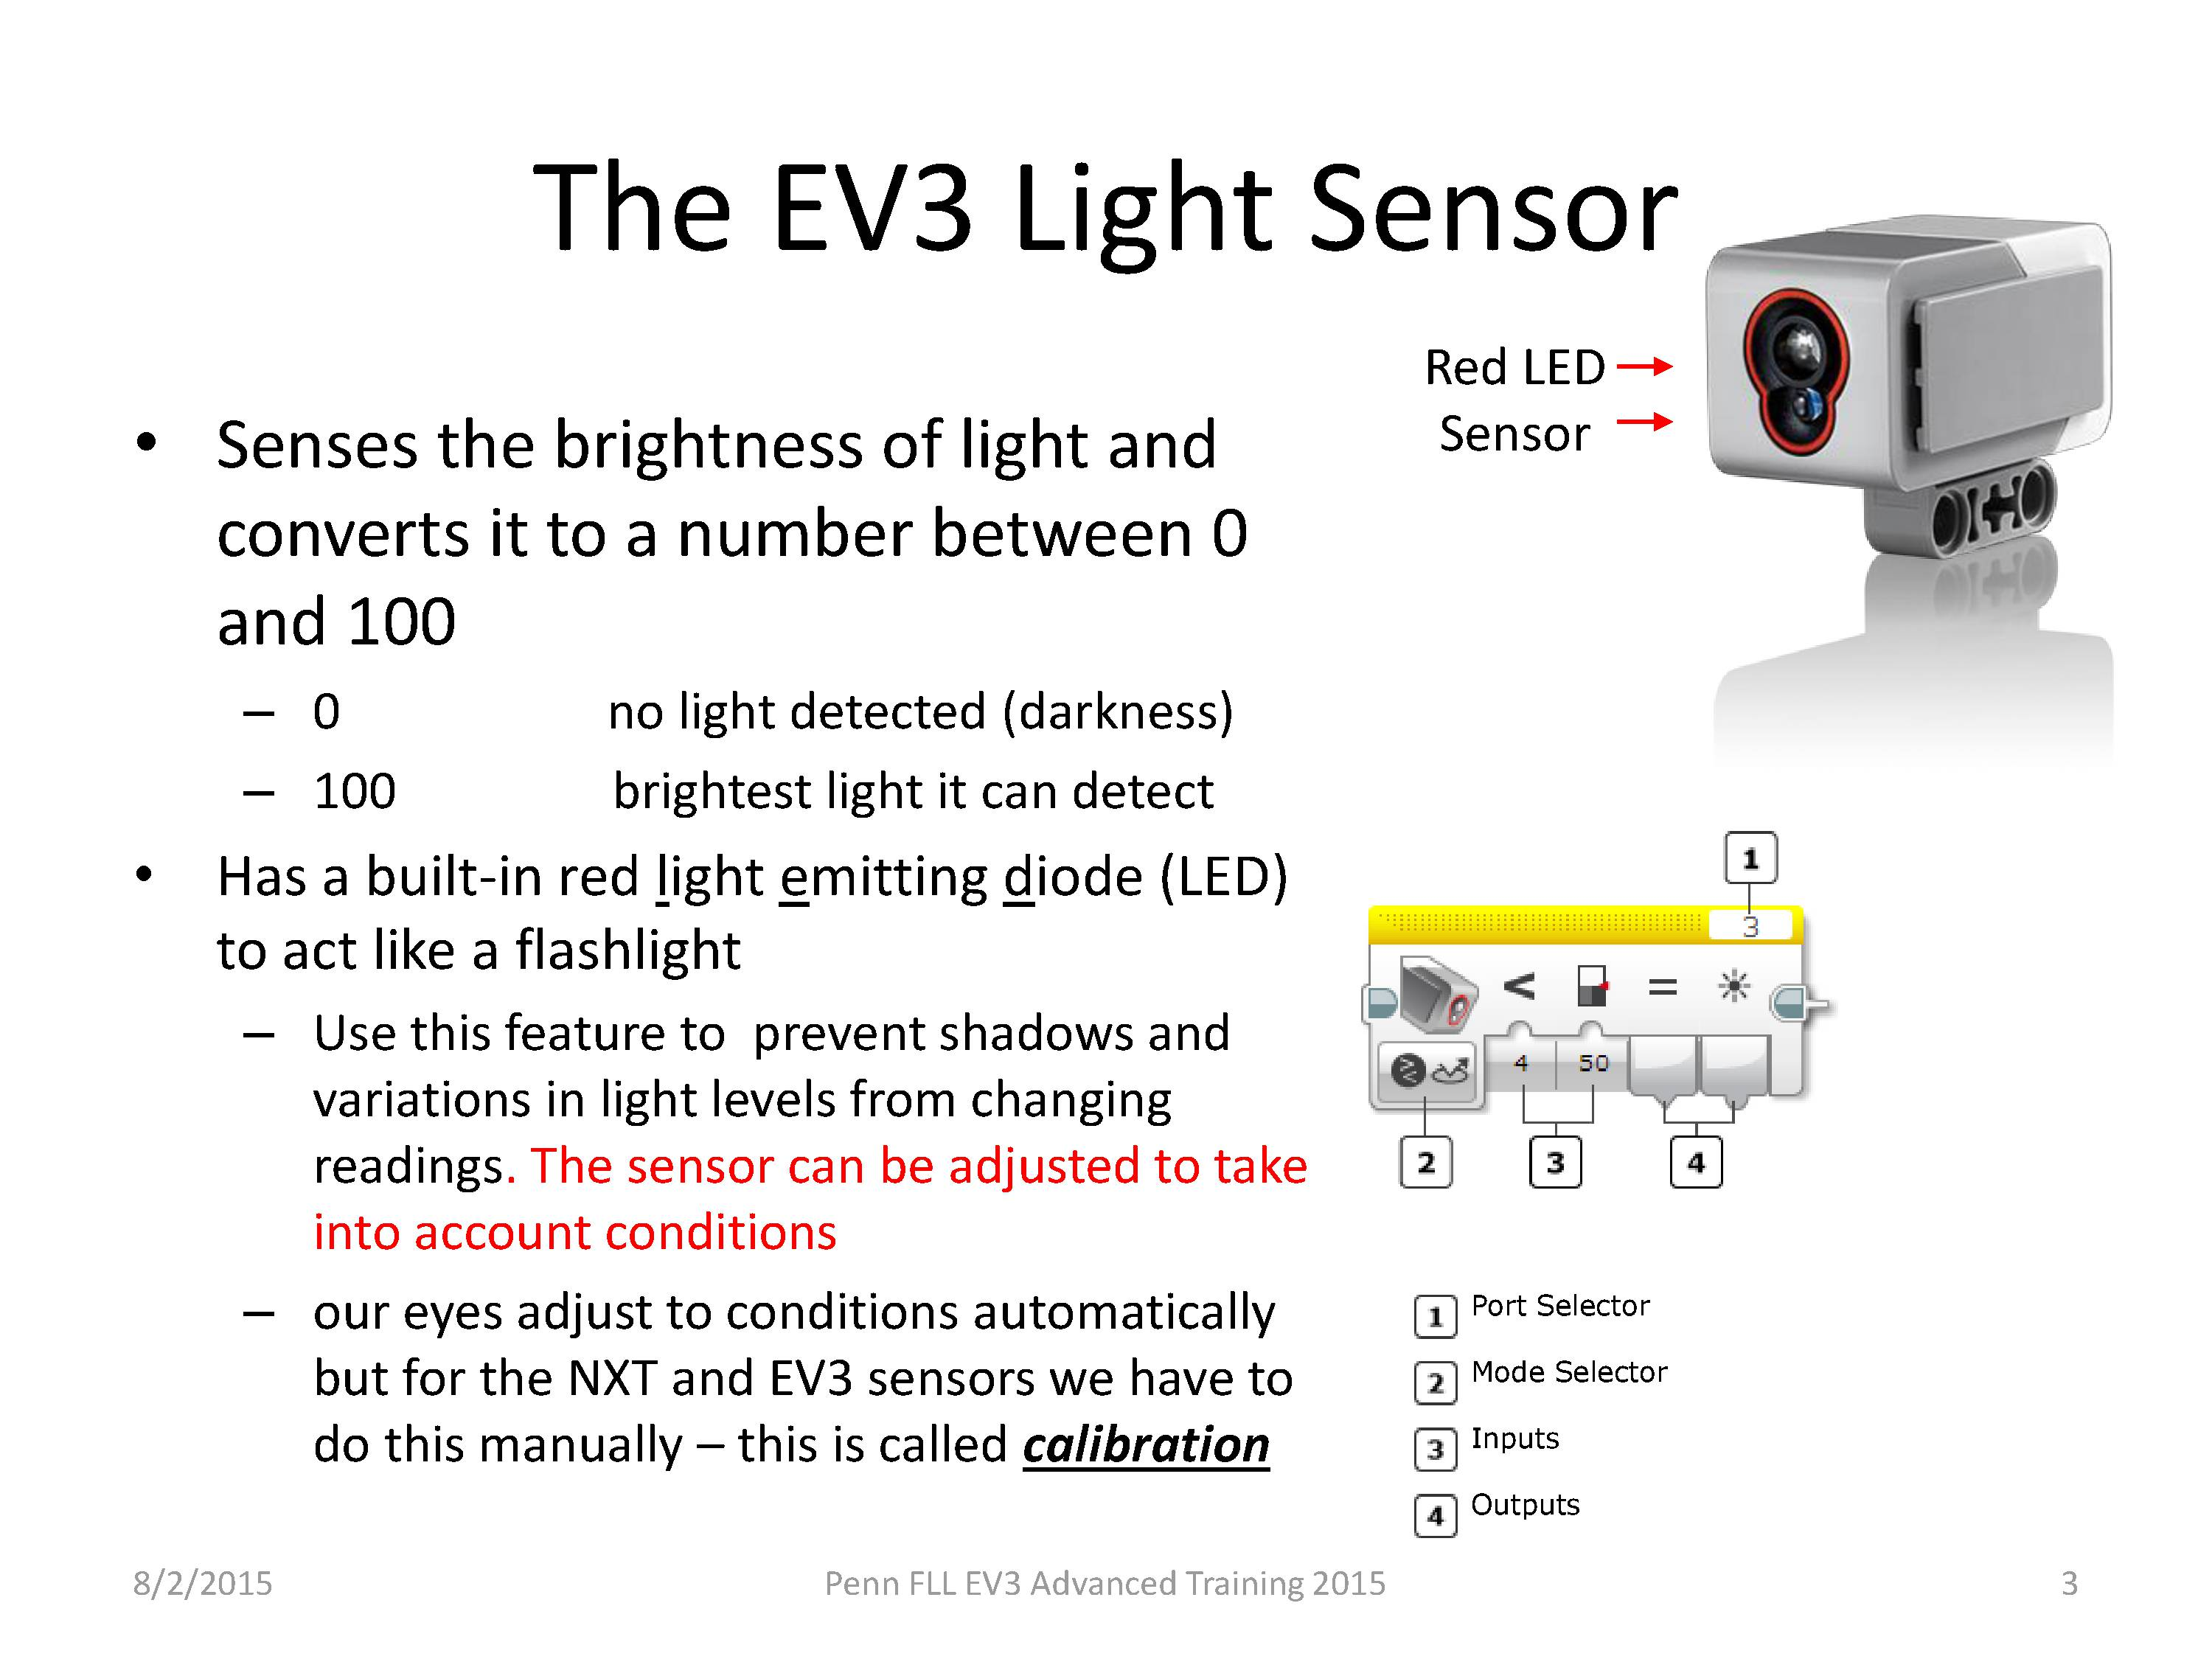
\includegraphics[scale=0.4]{ev3advanced2015/file-page3}
%\caption{lion!!}
\end{figure}
\end{frame}

\begin{frame}
%\frametitle{What we need to make a robot follow a line}
\begin{figure}
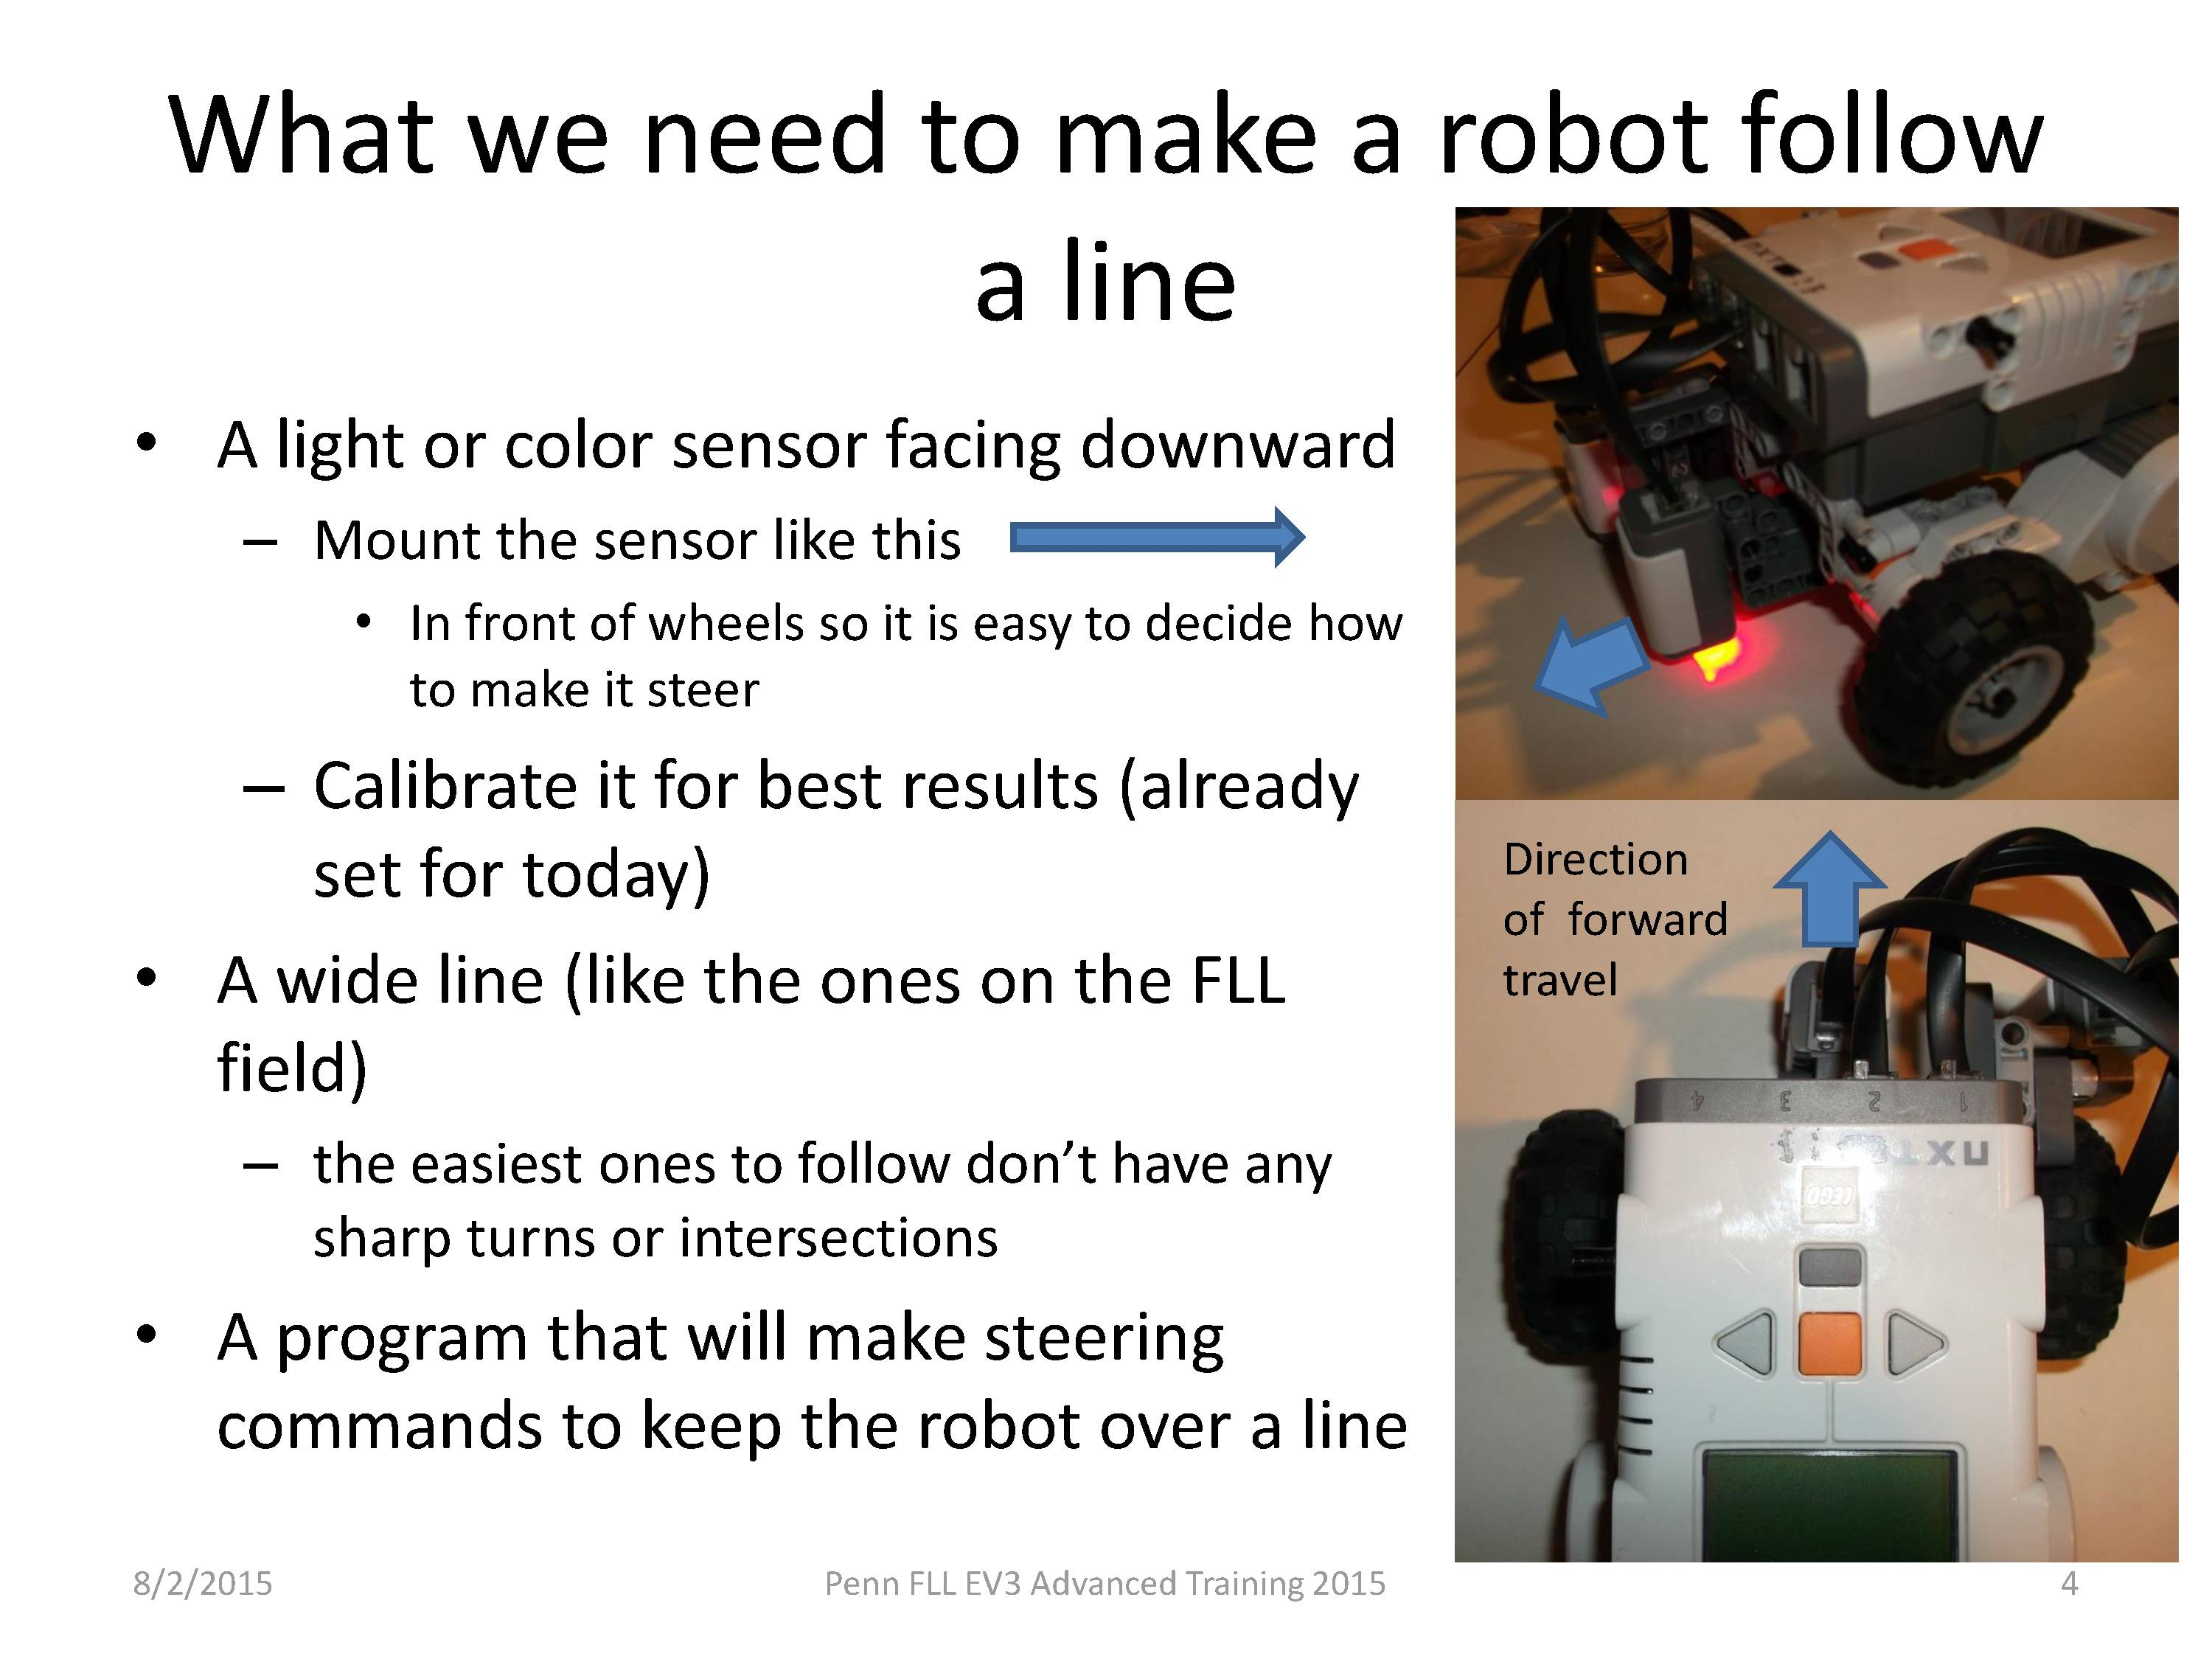
\includegraphics[scale=0.4]{ev3advanced2015/file-page4}
%\caption{lion!!}
\end{figure}
\end{frame}

\begin{frame}
%\frametitle{How the ligth sensor reacts}
\begin{figure}
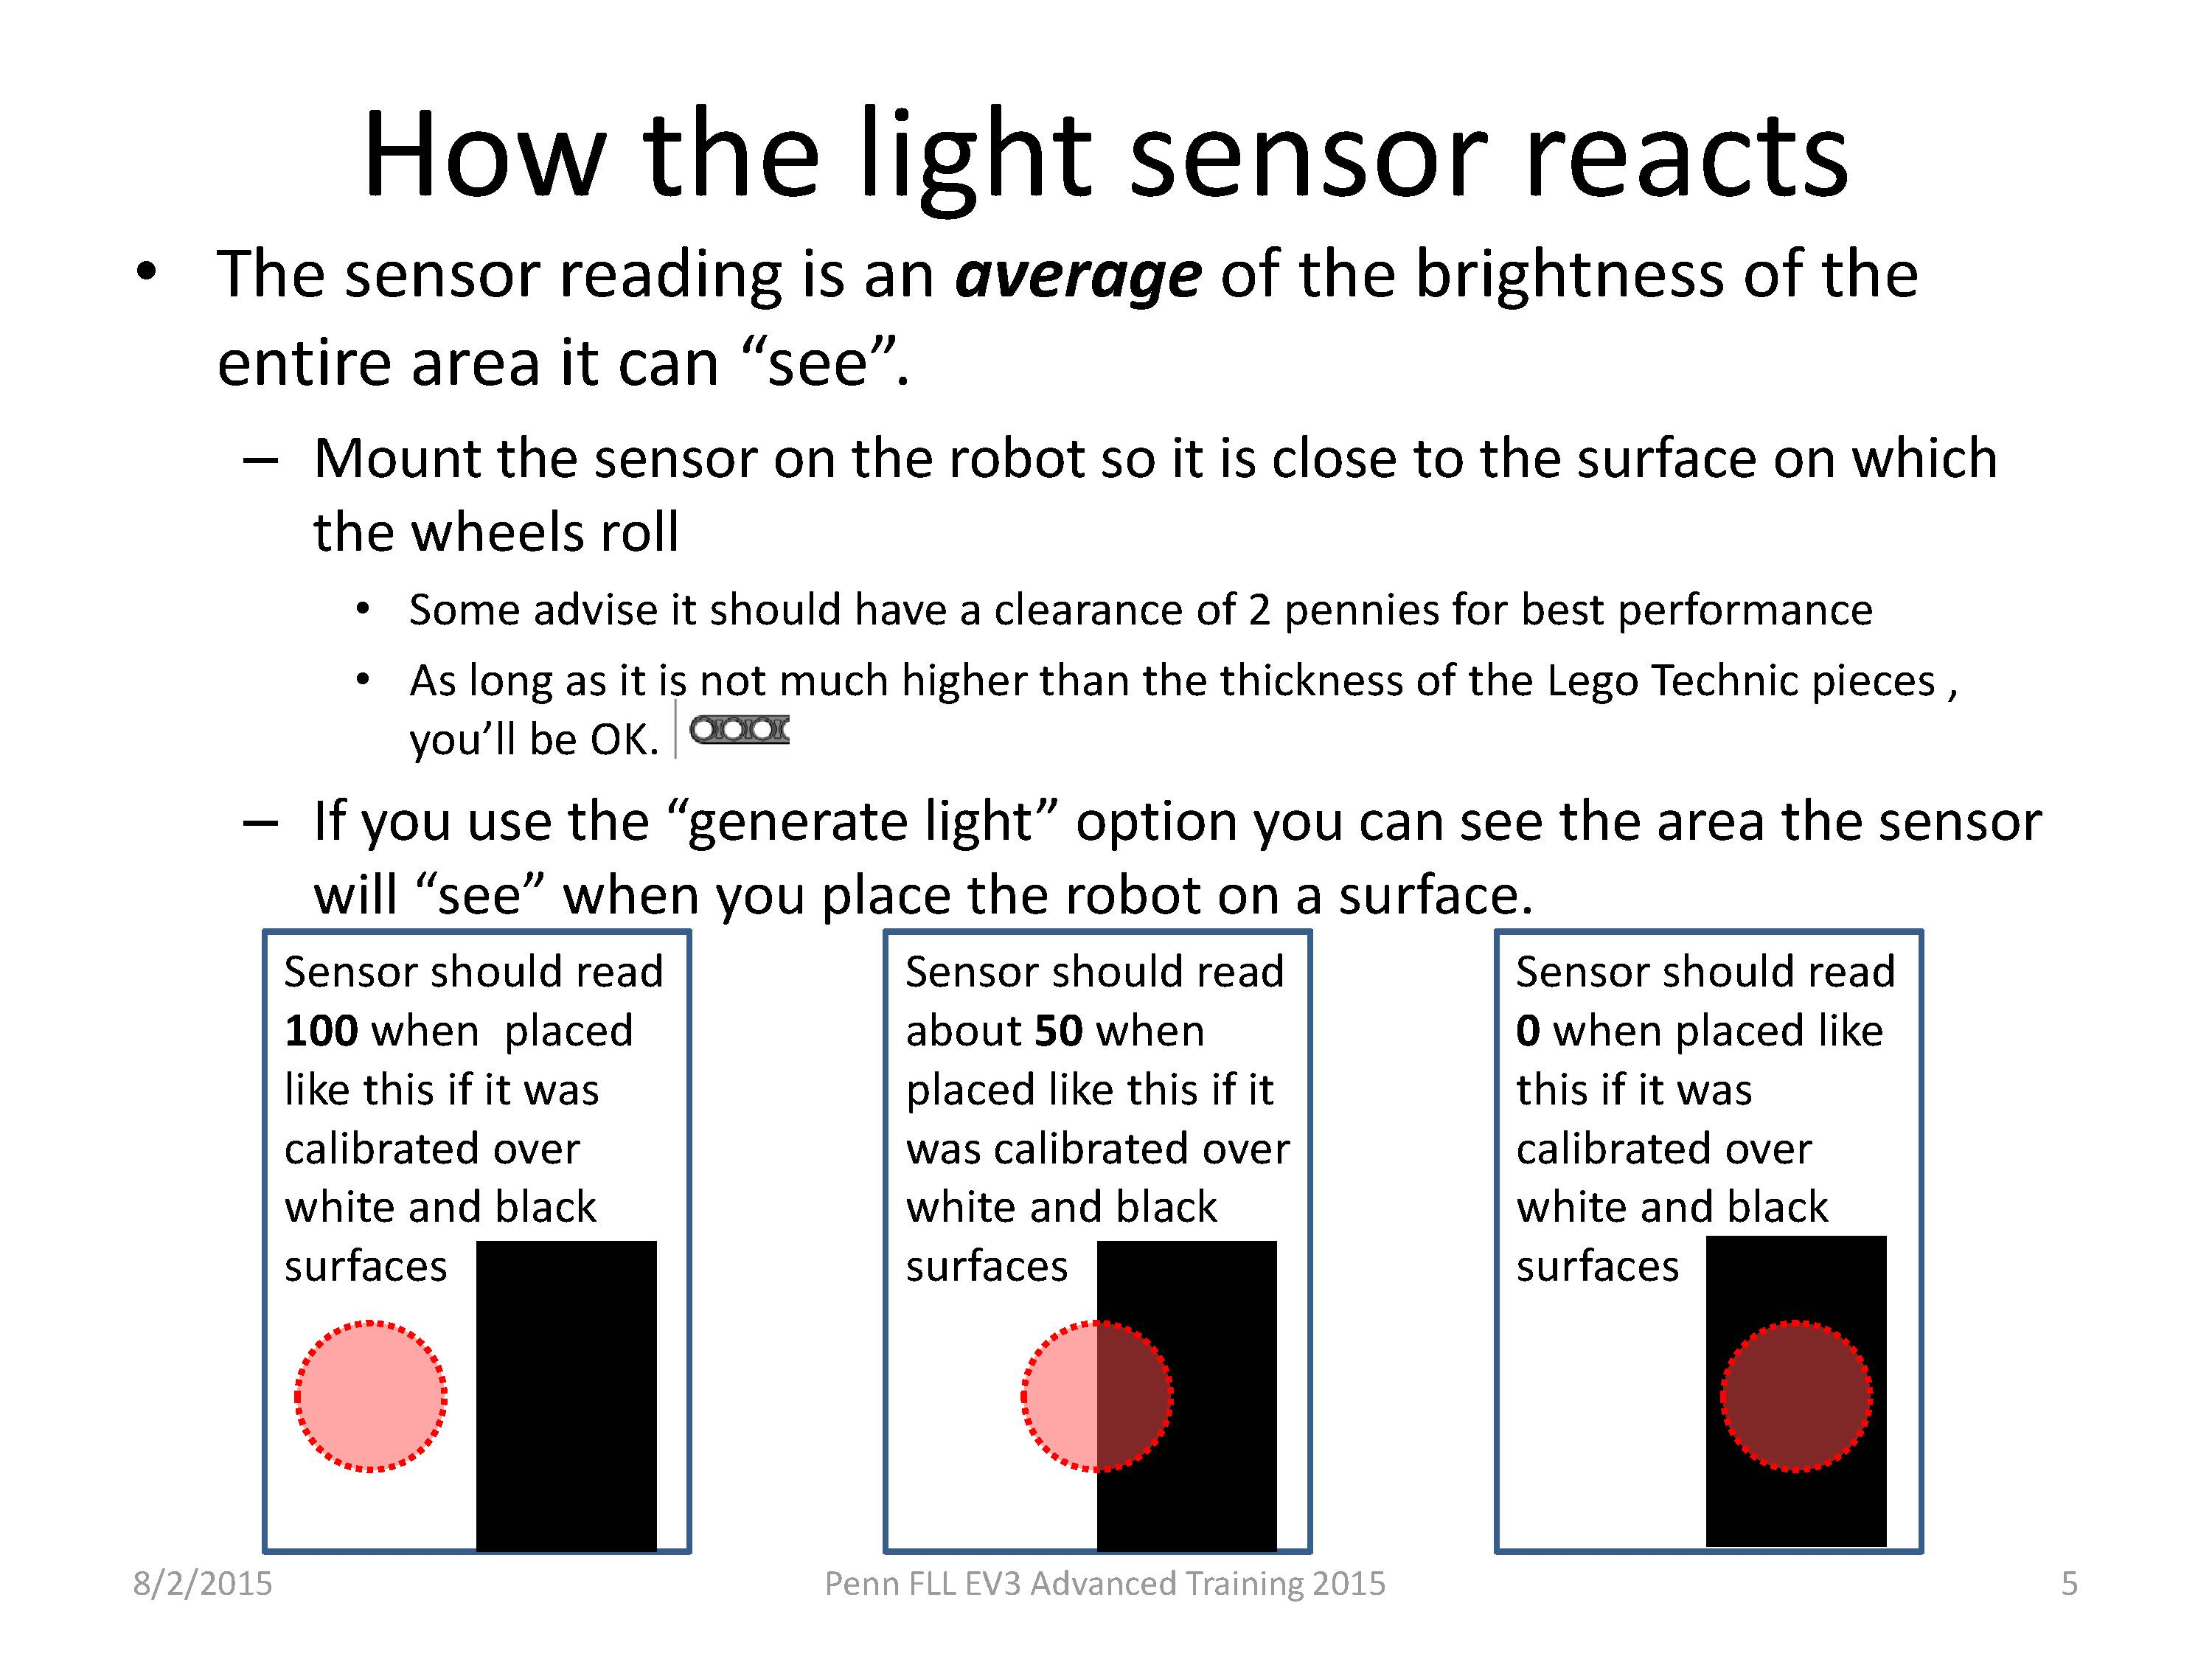
\includegraphics[scale=0.4]{ev3advanced2015/file-page5}
%\caption{lion!!}
\end{figure}
\end{frame}

\begin{frame}
%\frametitle{Pictures}
\begin{figure}
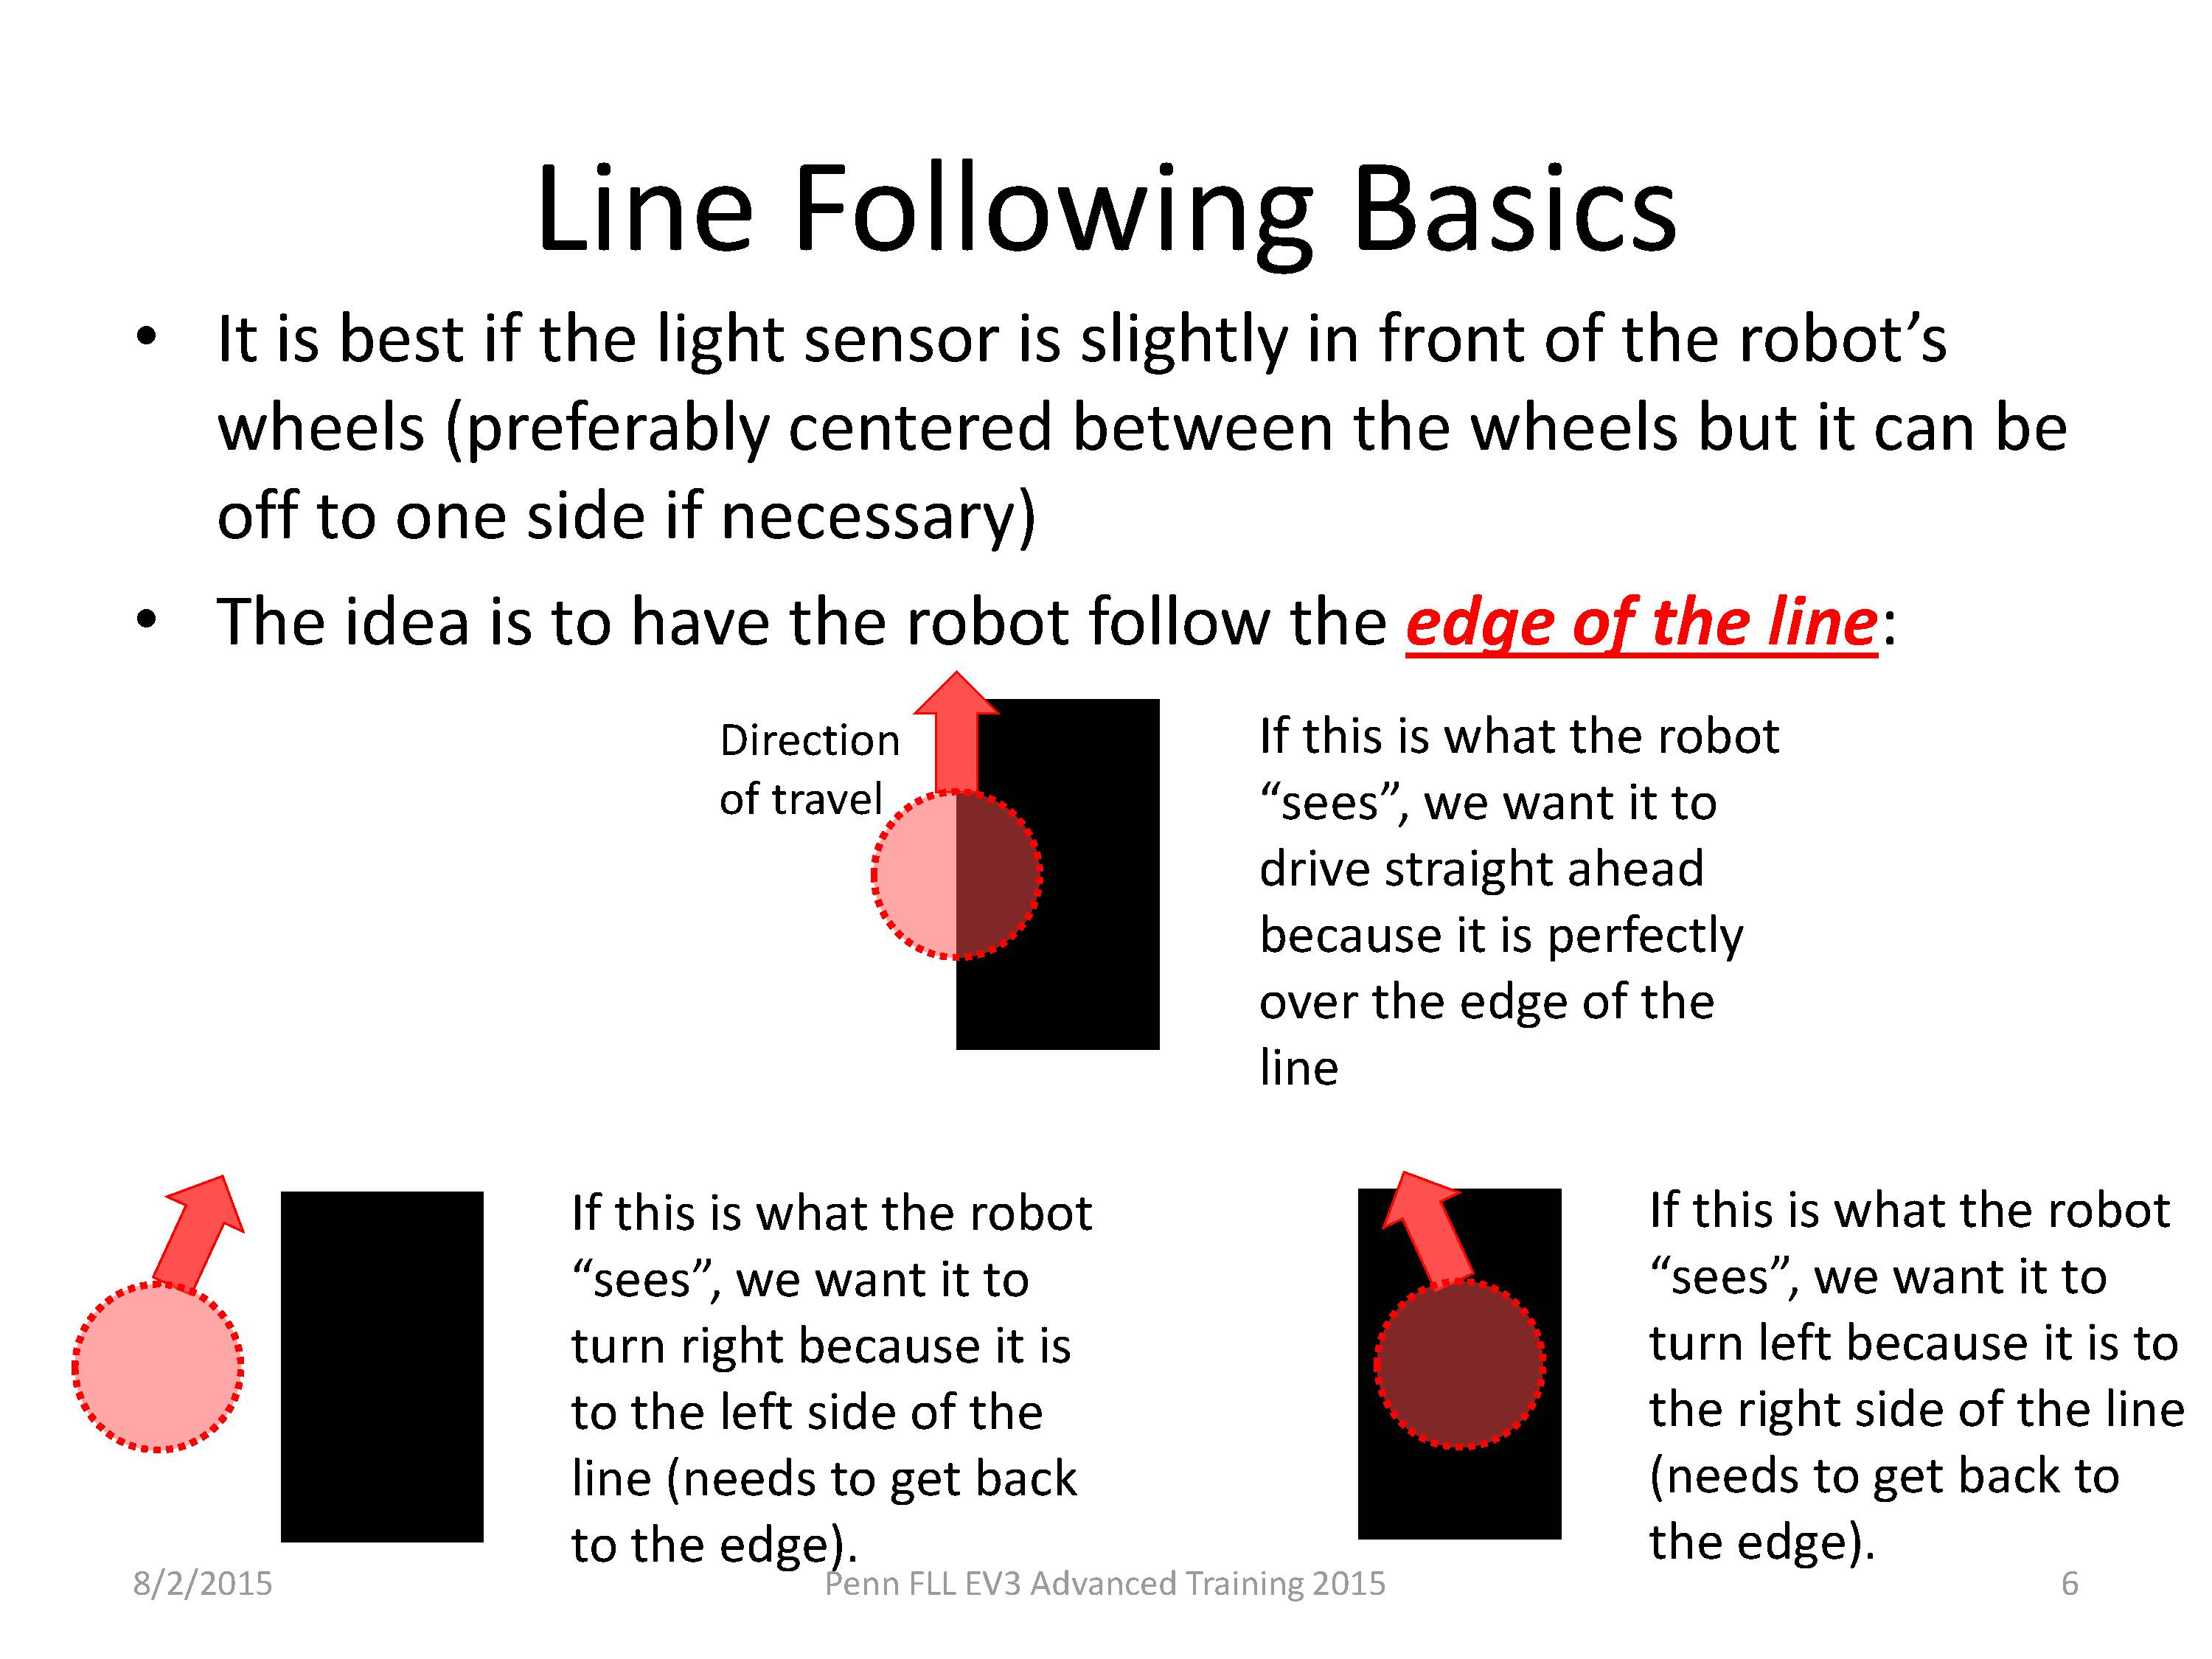
\includegraphics[scale=0.4]{ev3advanced2015/file-page6}
%\caption{lion!!}
\end{figure}
\end{frame}

\begin{frame}
%\frametitle{Pictures}
\begin{figure}
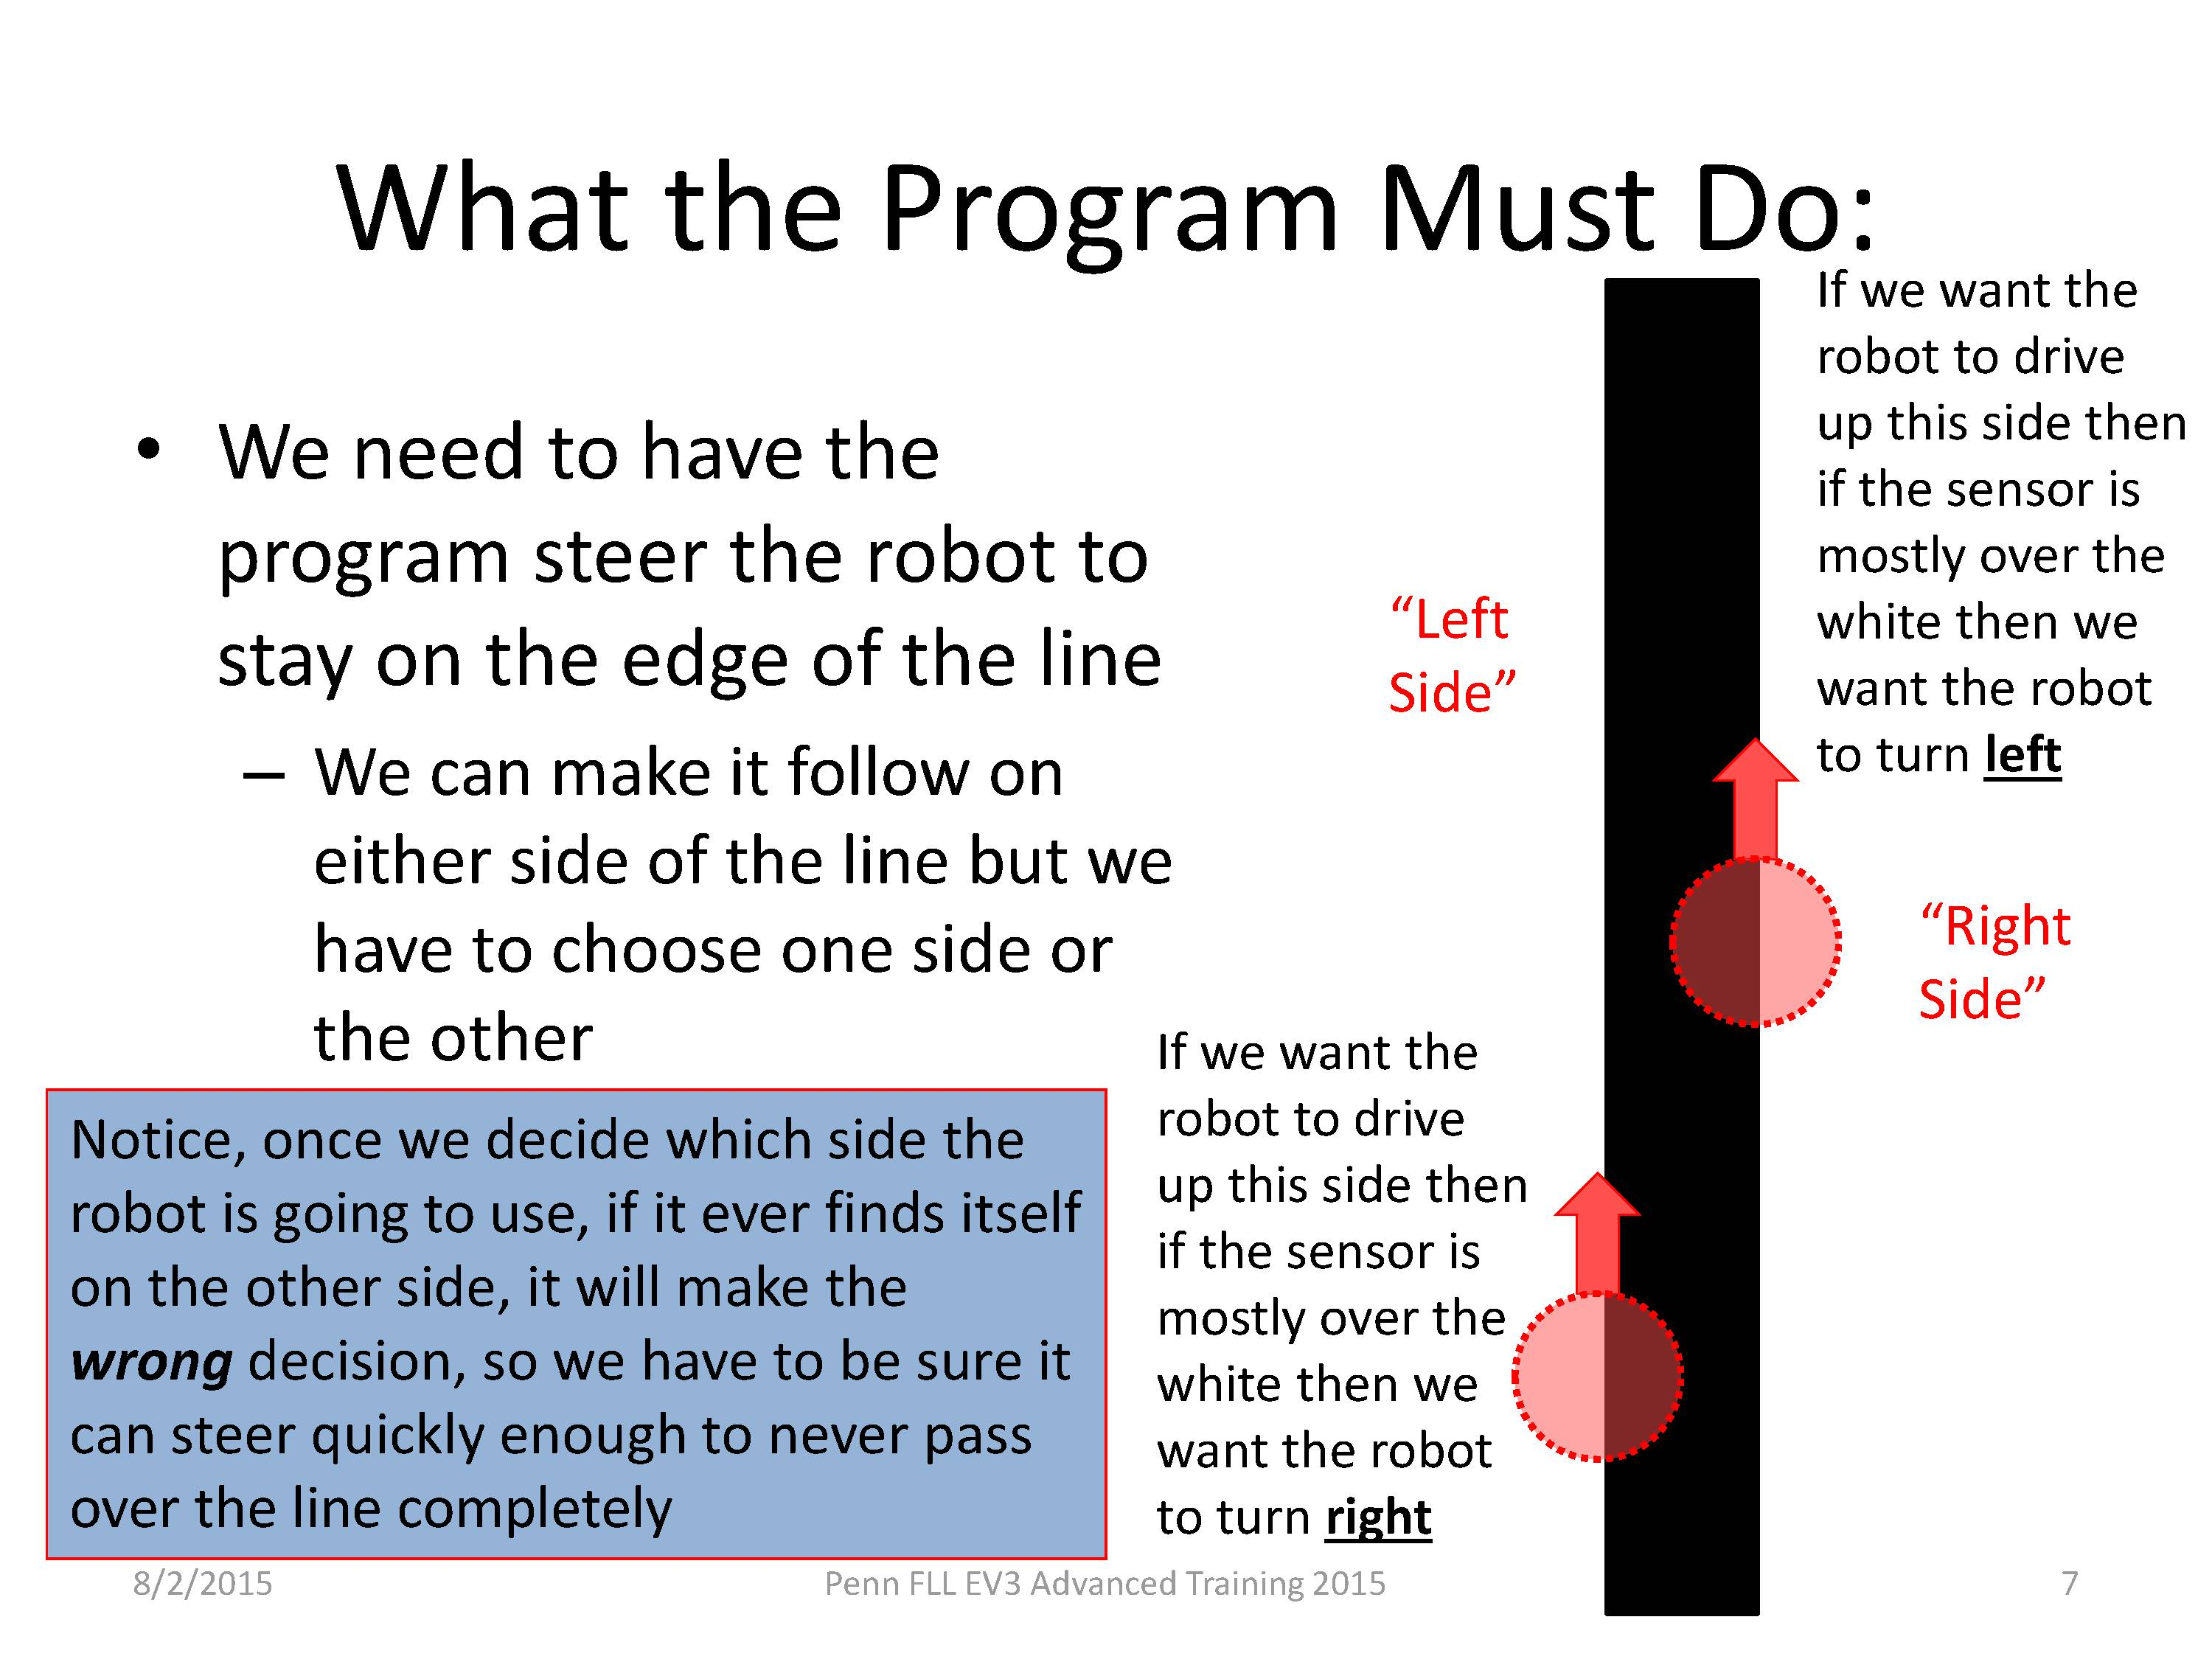
\includegraphics[scale=0.4]{ev3advanced2015/file-page7}
%\caption{lion!!}
\end{figure}
\end{frame}

\begin{frame}
%\frametitle{Pictures}
\begin{figure}
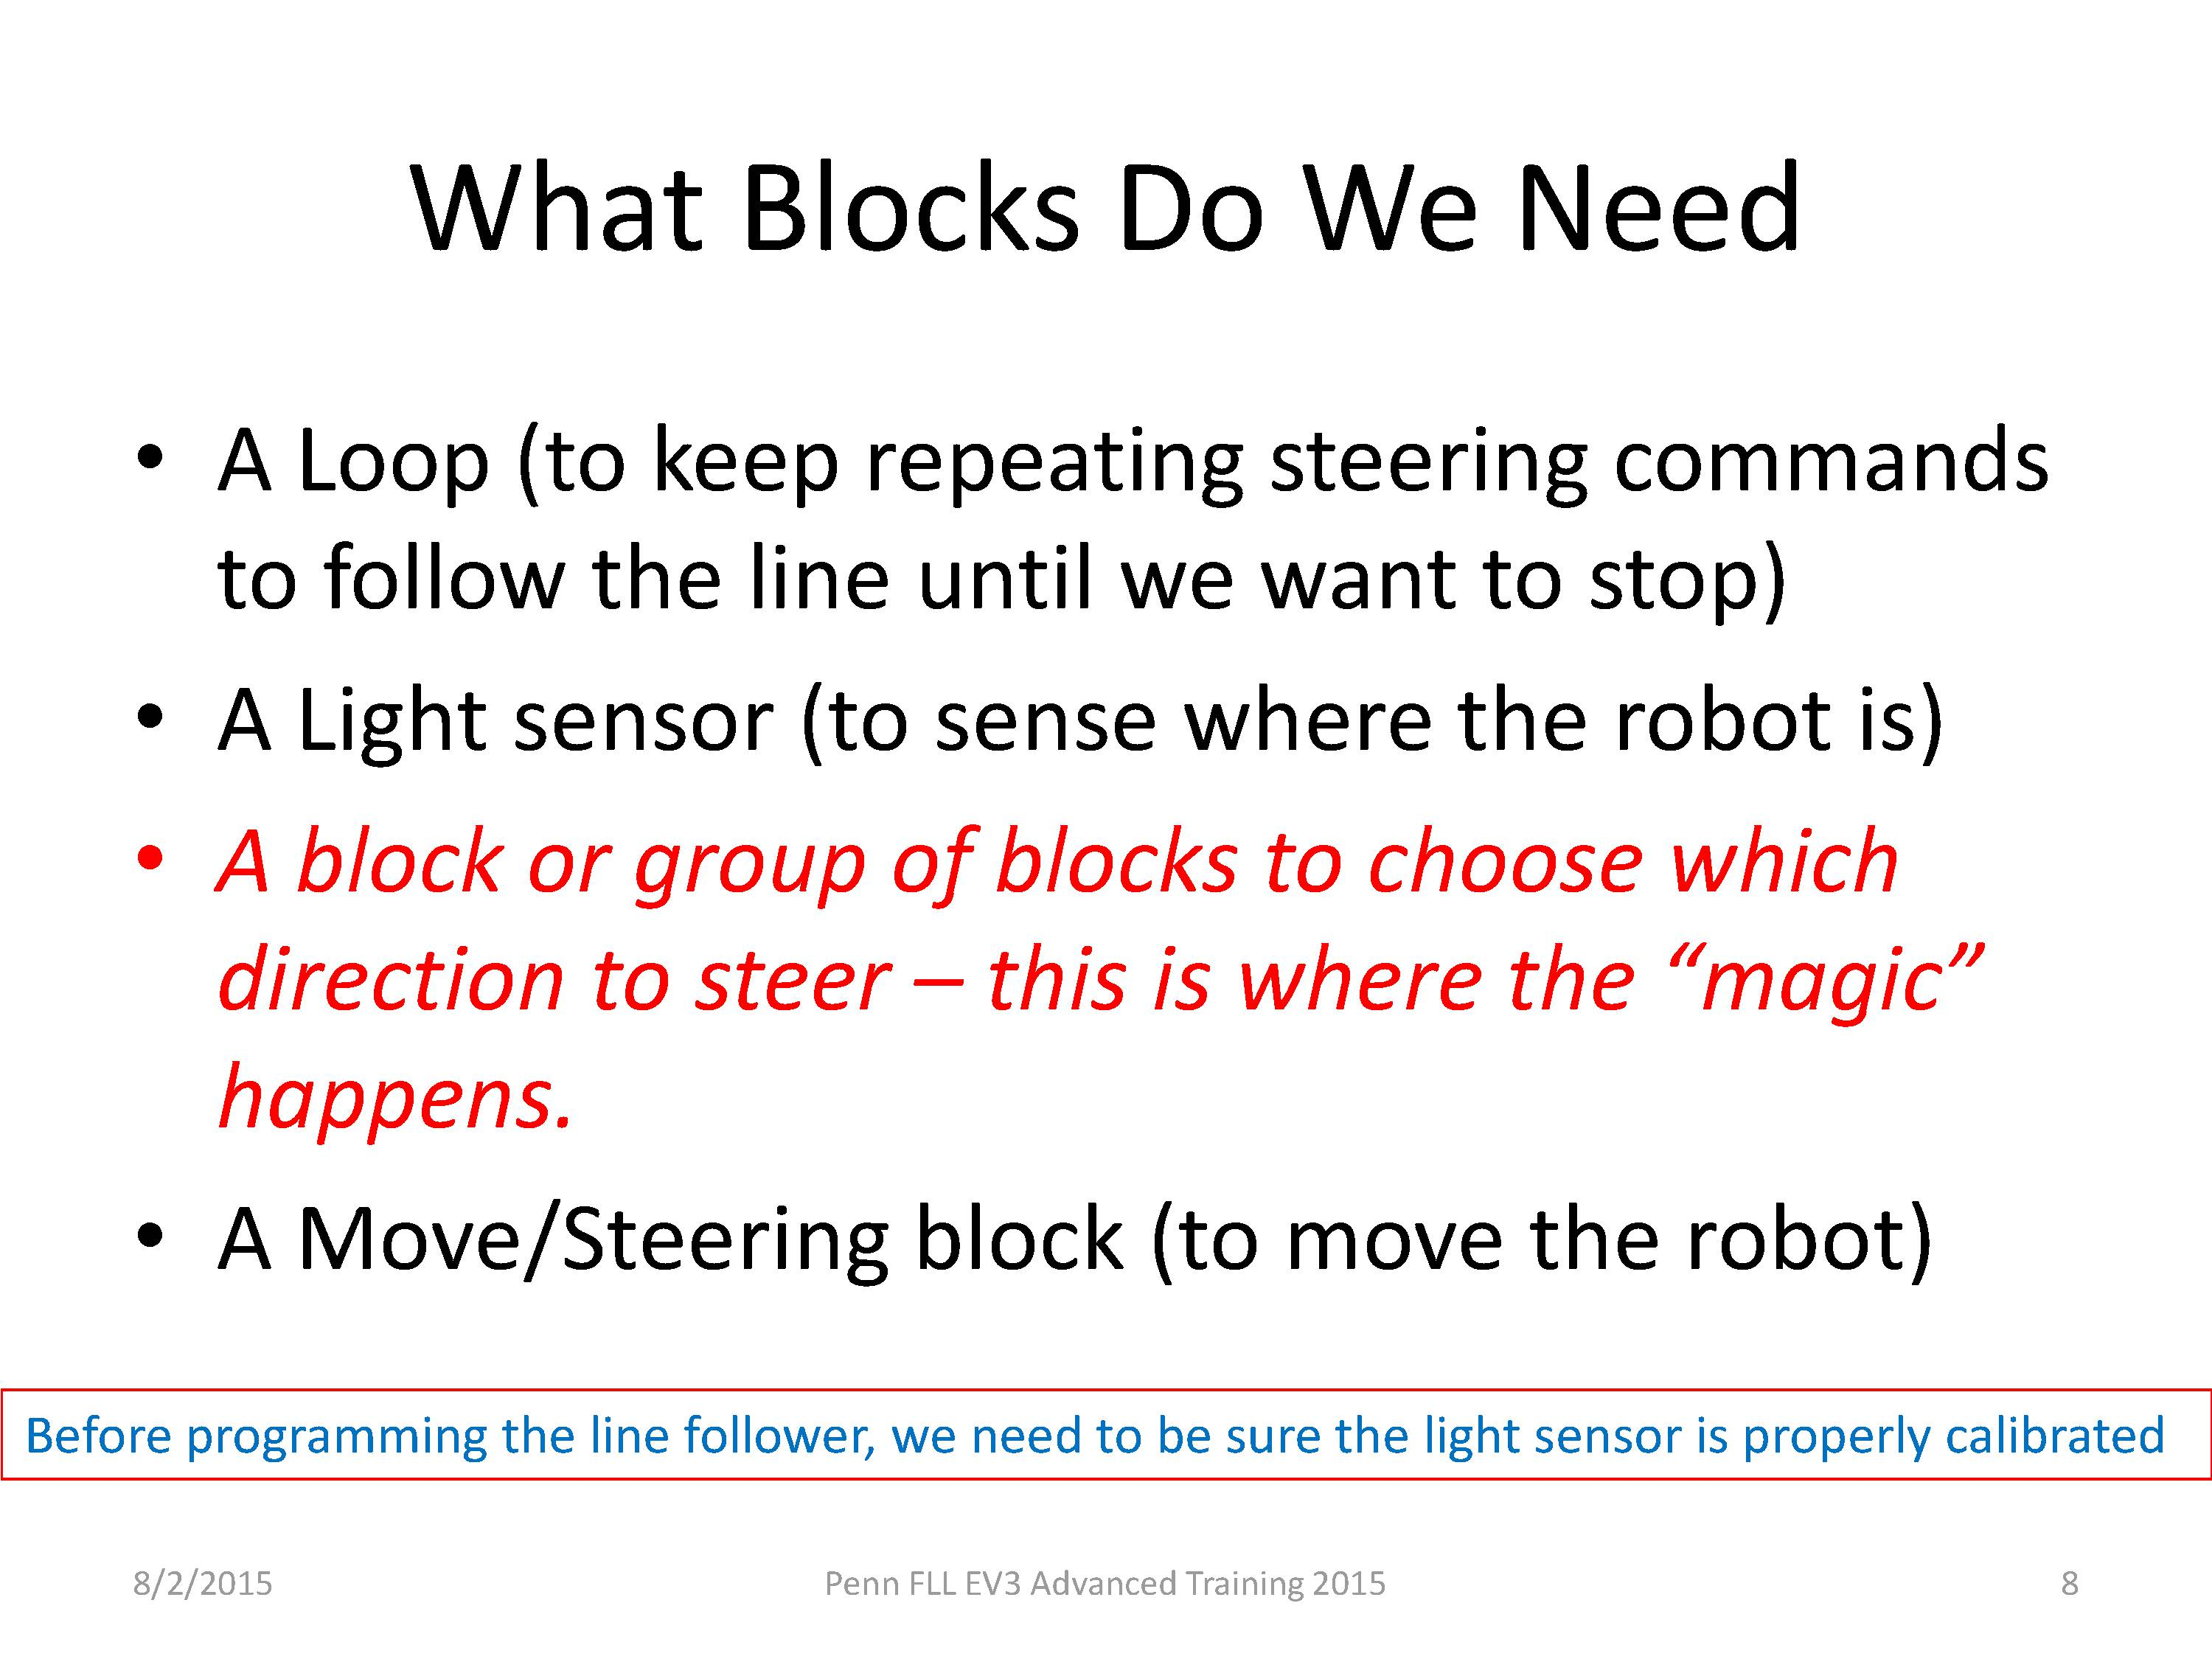
\includegraphics[scale=0.4]{ev3advanced2015/file-page8}
%\caption{lion!!}
\end{figure}
\end{frame}

\begin{frame}
%\frametitle{Pictures}
\begin{figure}
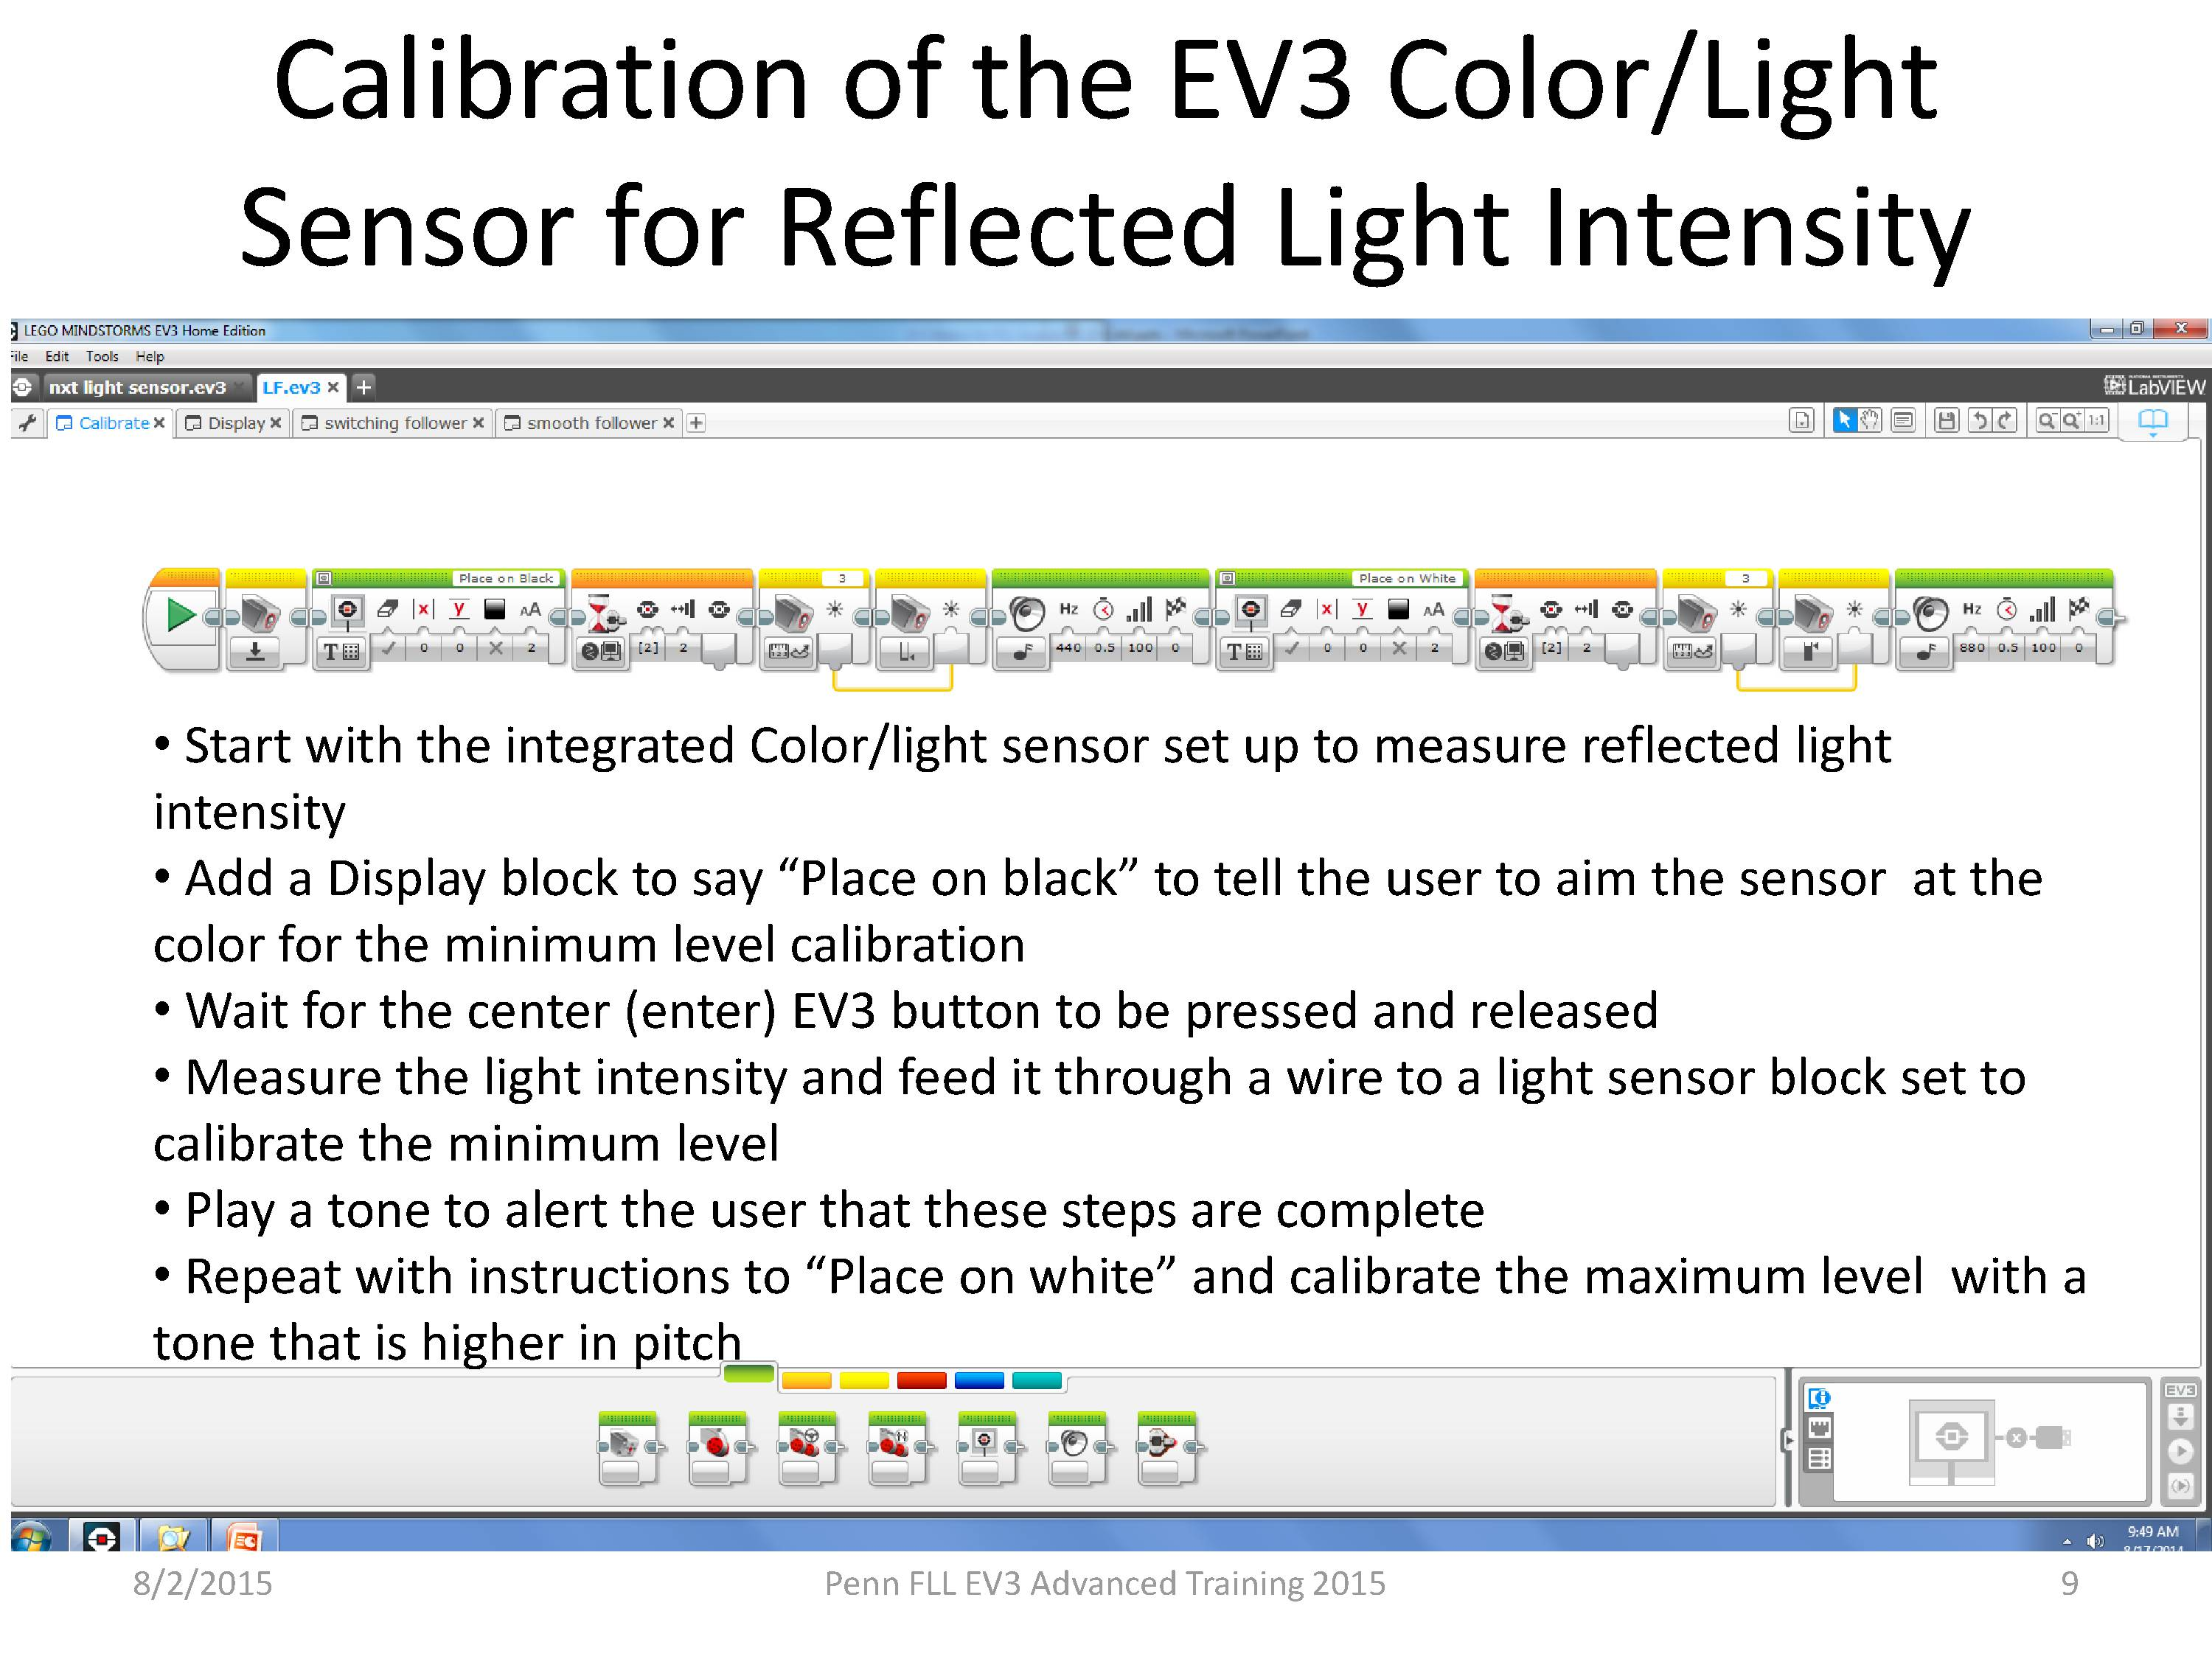
\includegraphics[scale=0.4]{ev3advanced2015/file-page9}
%\caption{lion!!}
\end{figure}
\end{frame}

\begin{frame}
%\frametitle{Pictures}
\begin{figure}
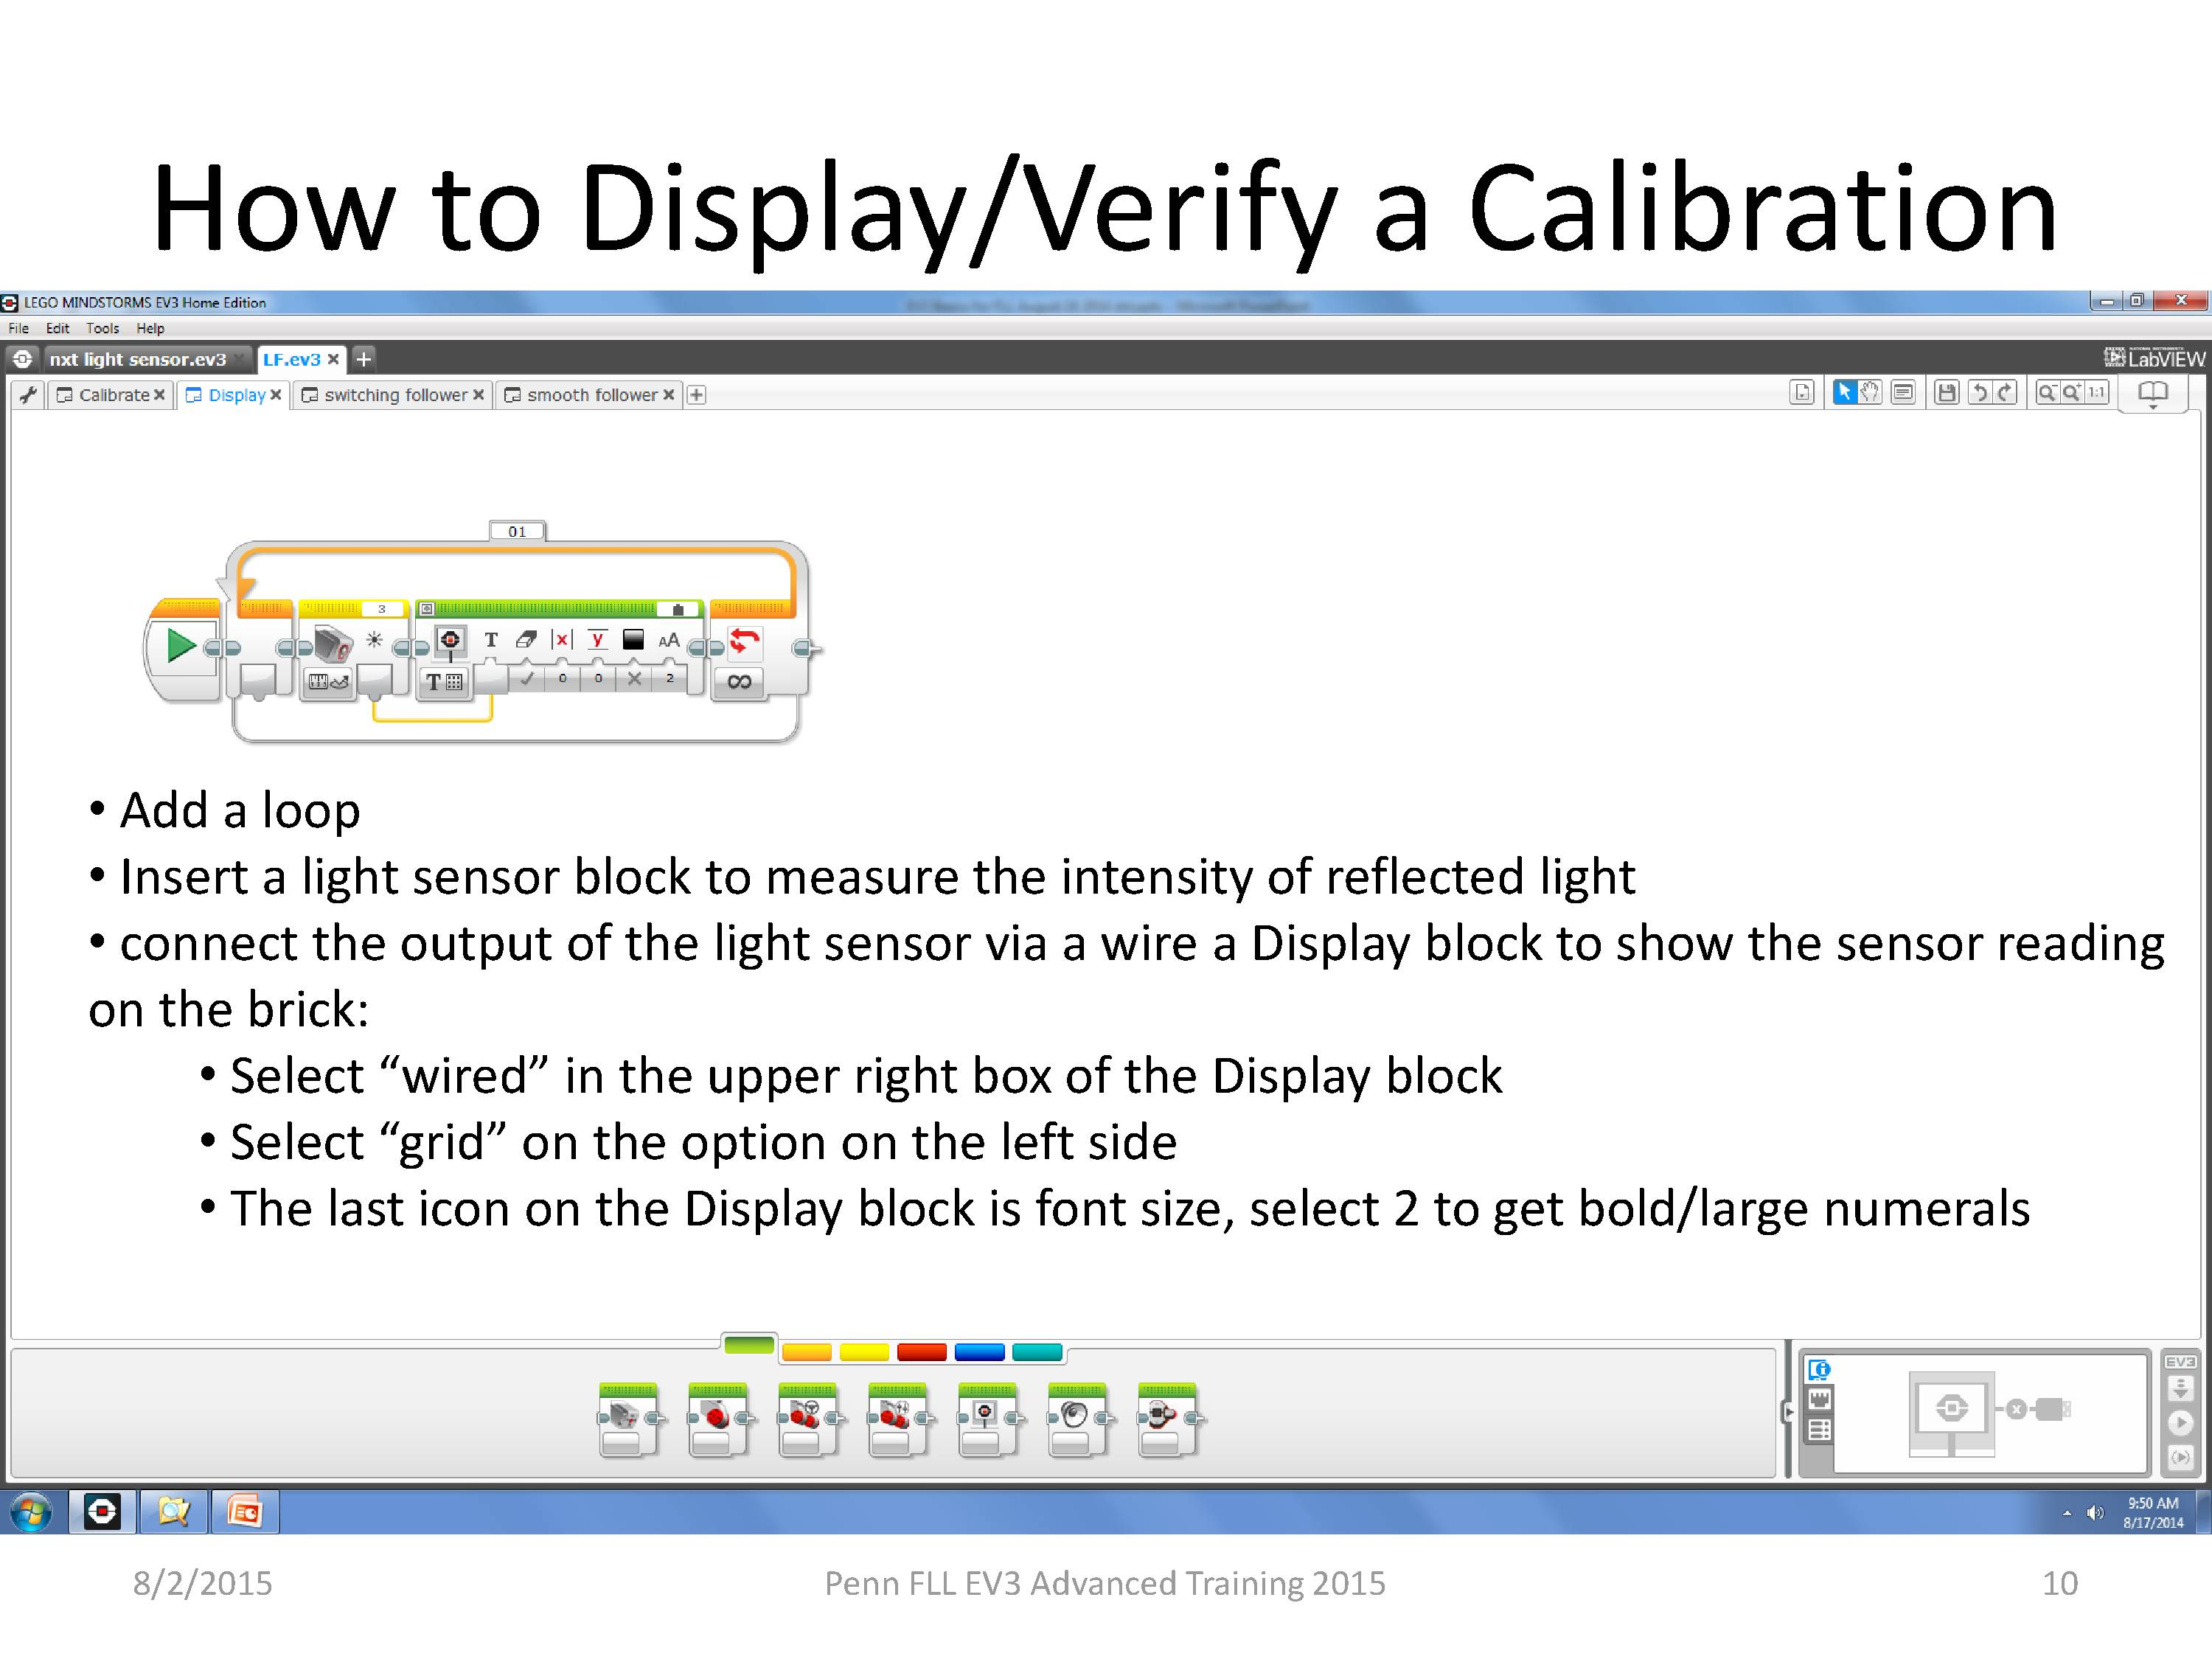
\includegraphics[scale=0.4]{ev3advanced2015/file-page10}
%\caption{lion!!}
\end{figure}
\end{frame}

\begin{frame}
%\frametitle{Pictures}
\begin{figure}
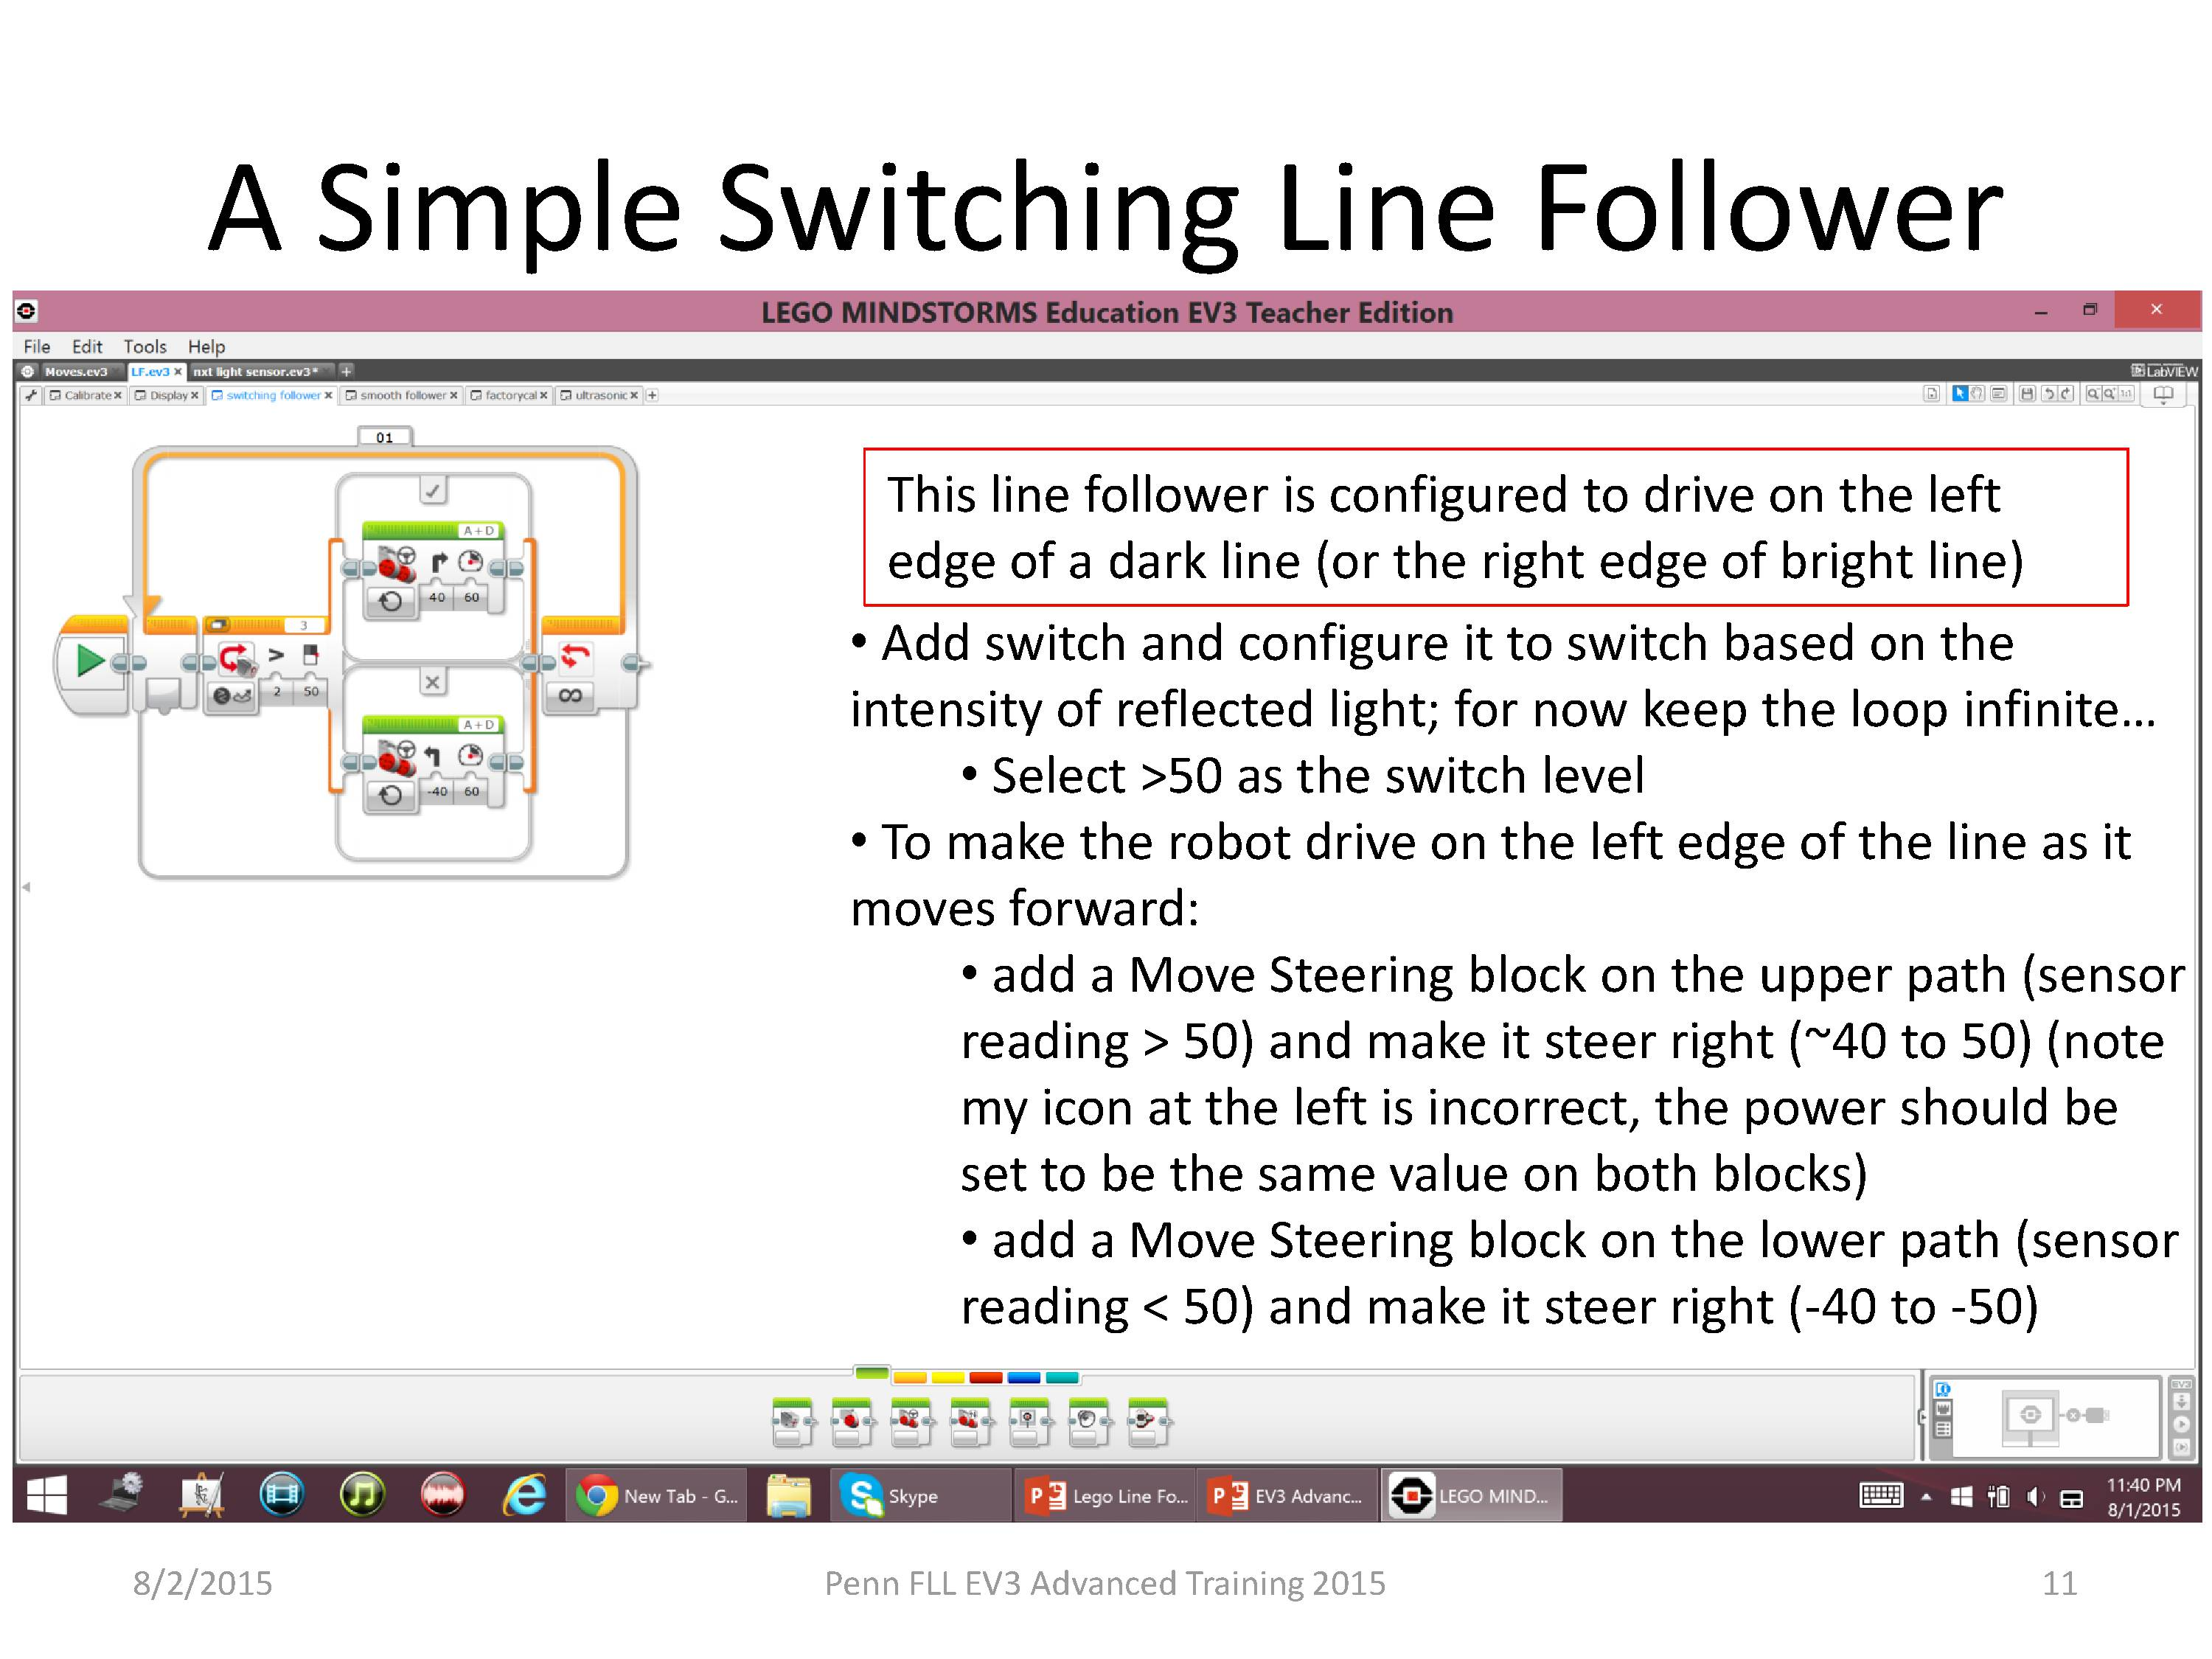
\includegraphics[scale=0.4]{ev3advanced2015/file-page11}
%\caption{lion!!}
\end{figure}

\end{frame}
\begin{frame}
%\frametitle{Pictures}
\begin{figure}
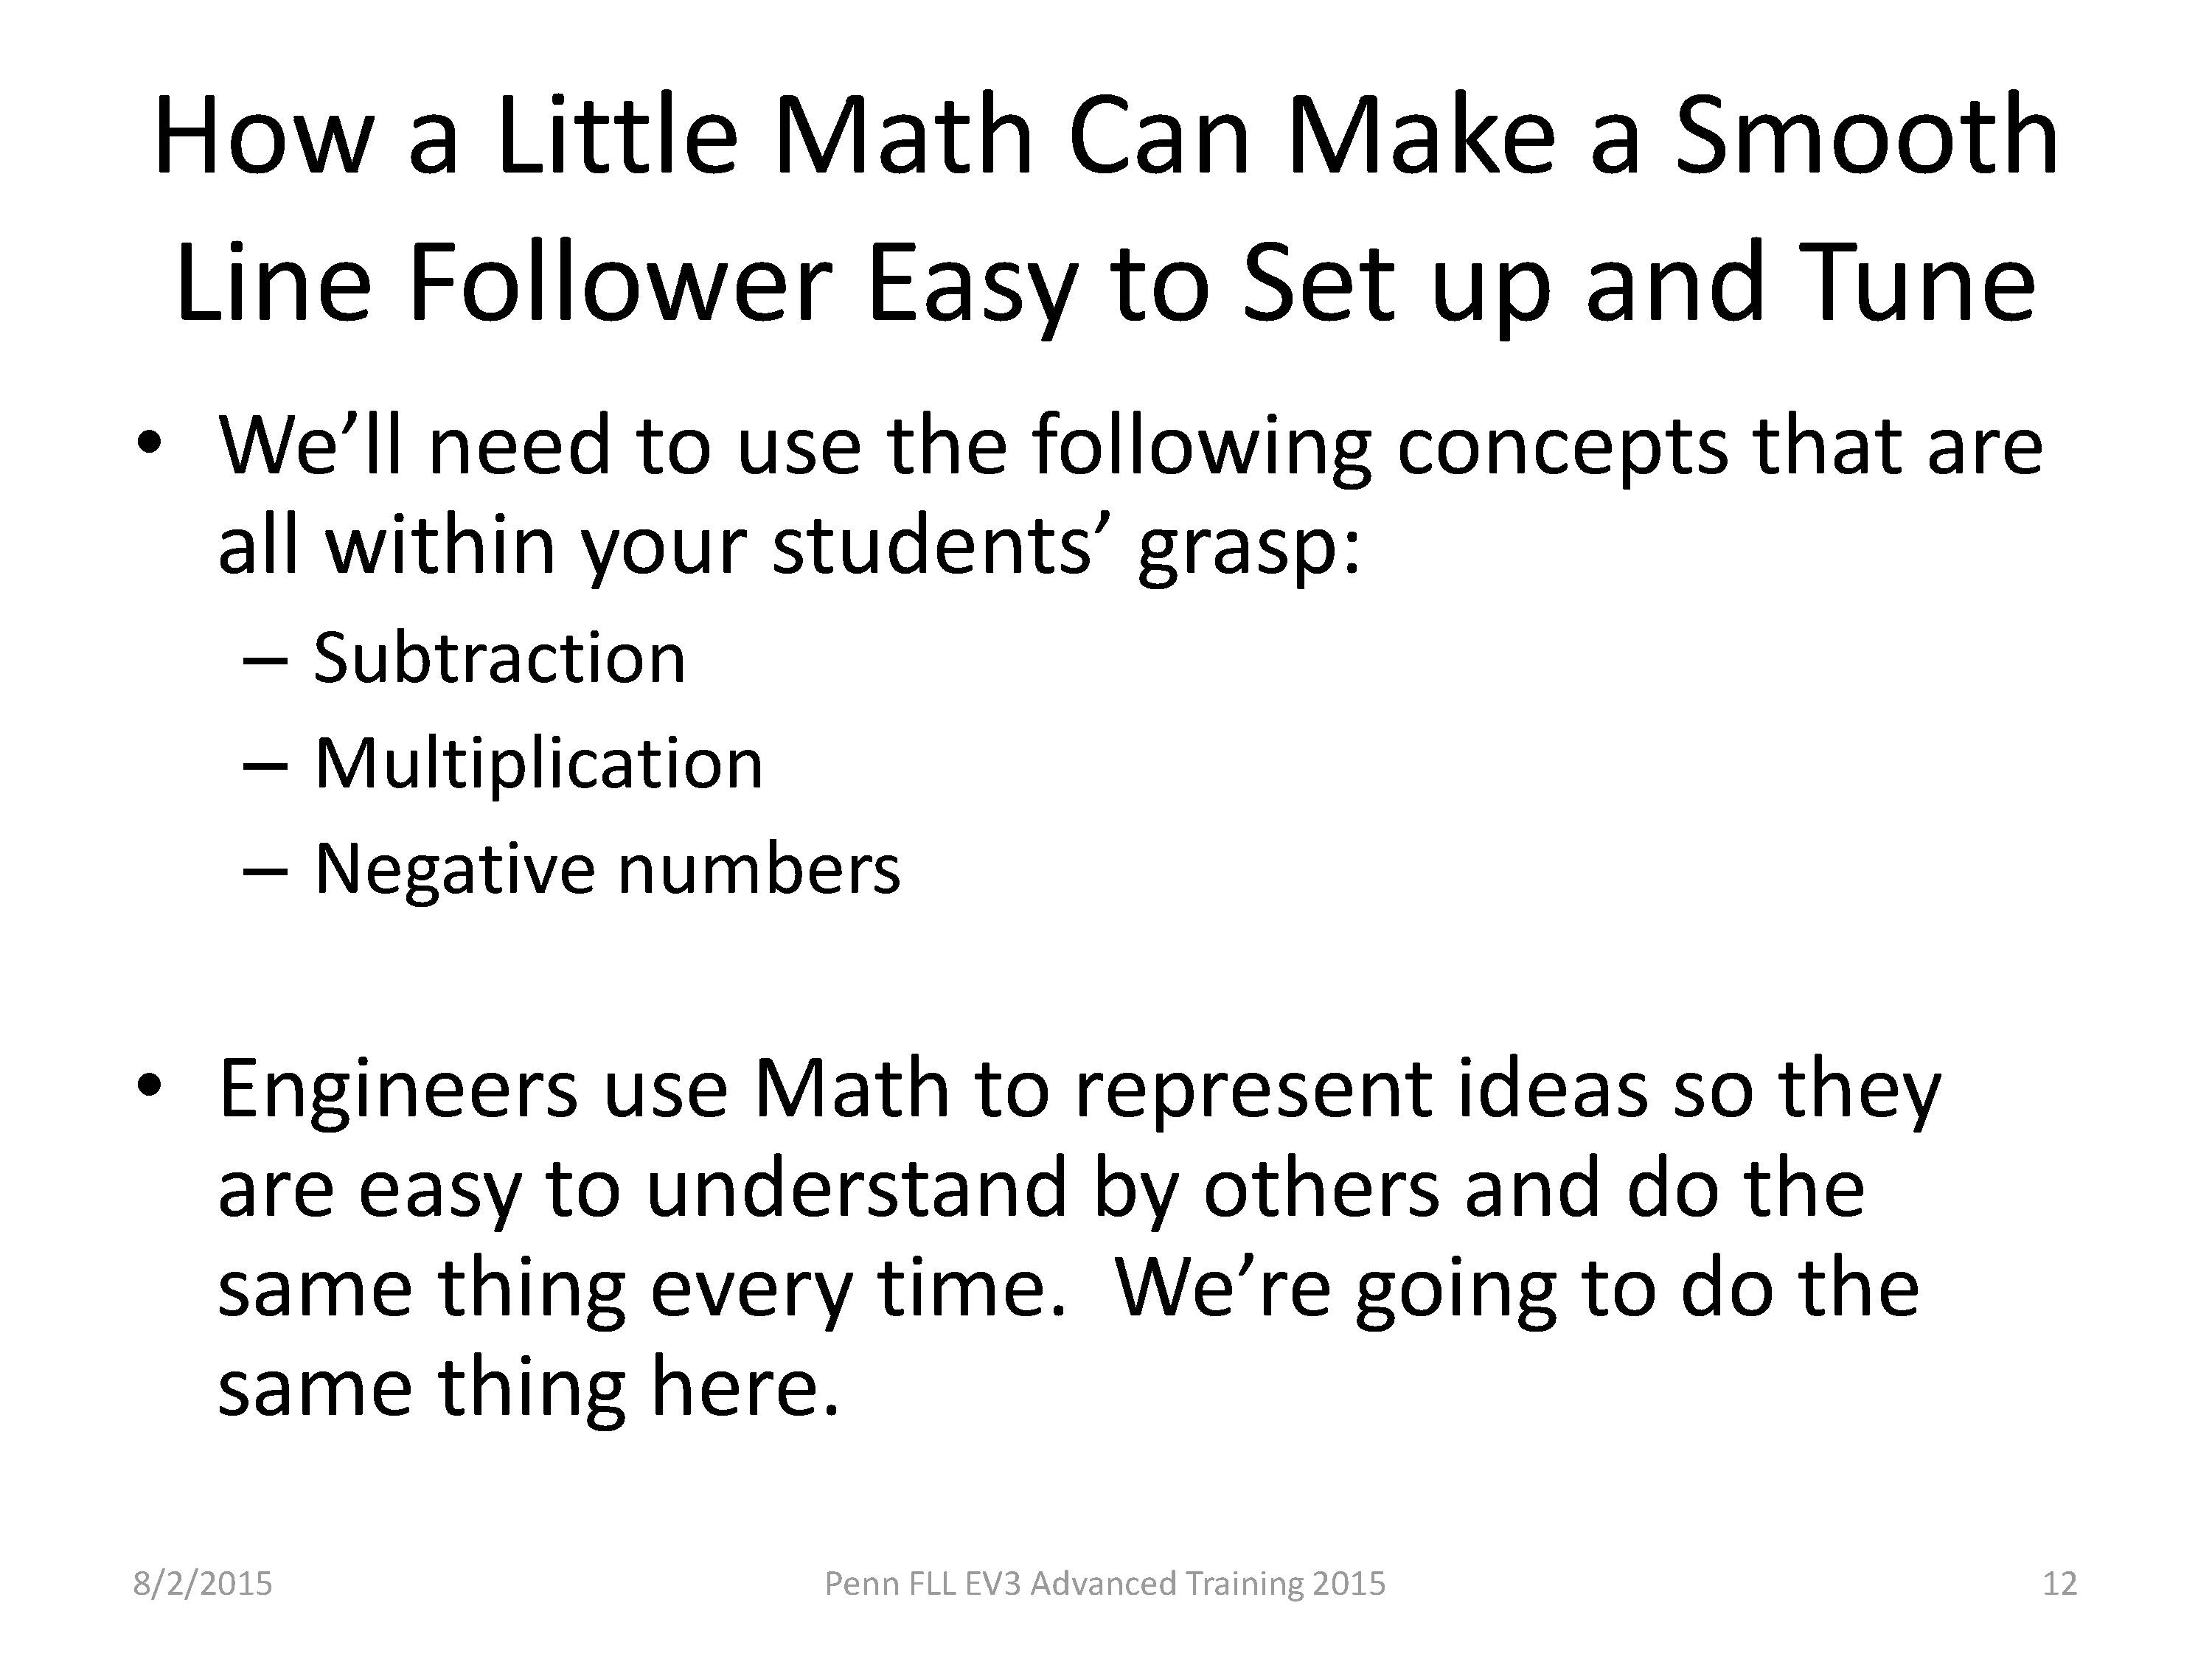
\includegraphics[scale=0.4]{ev3advanced2015/file-page12}
%\caption{lion!!}
\end{figure}
\end{frame}

\begin{frame}
%\frametitle{Pictures}
\begin{figure}
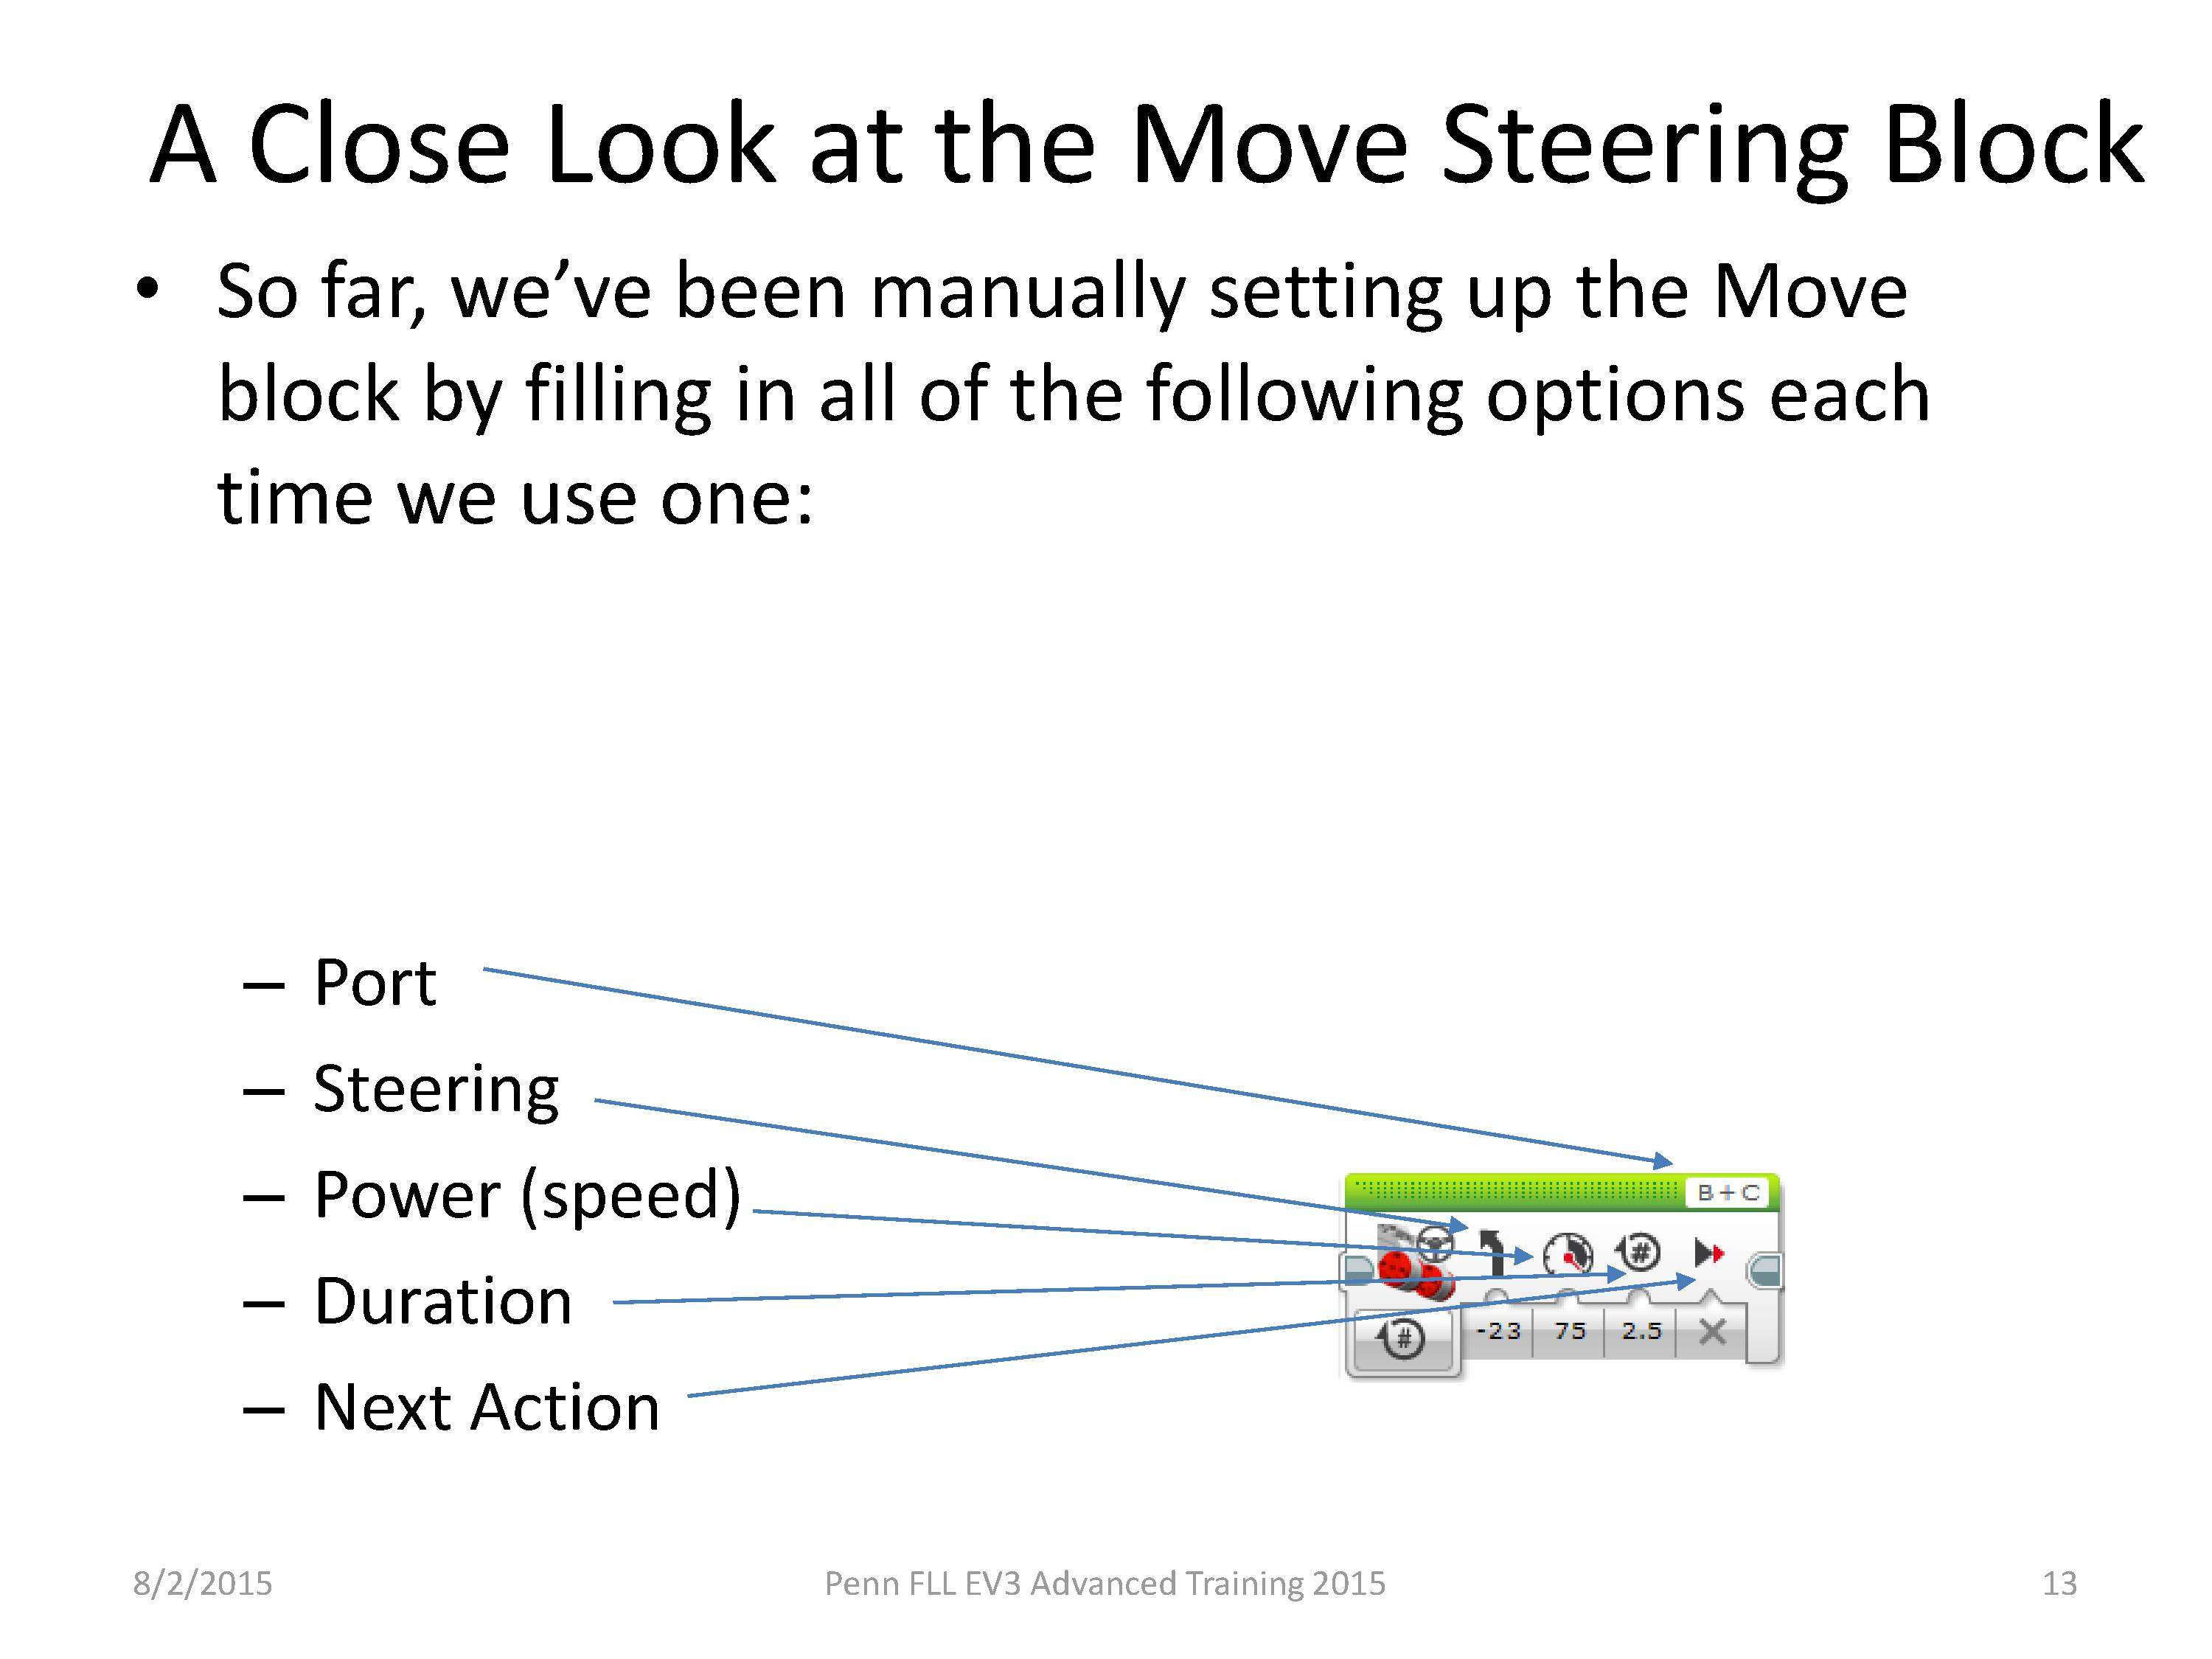
\includegraphics[scale=0.4]{ev3advanced2015/file-page13}
%\caption{lion!!}
\end{figure}
\end{frame}


\begin{frame}
%\frametitle{Pictures}
\begin{figure}
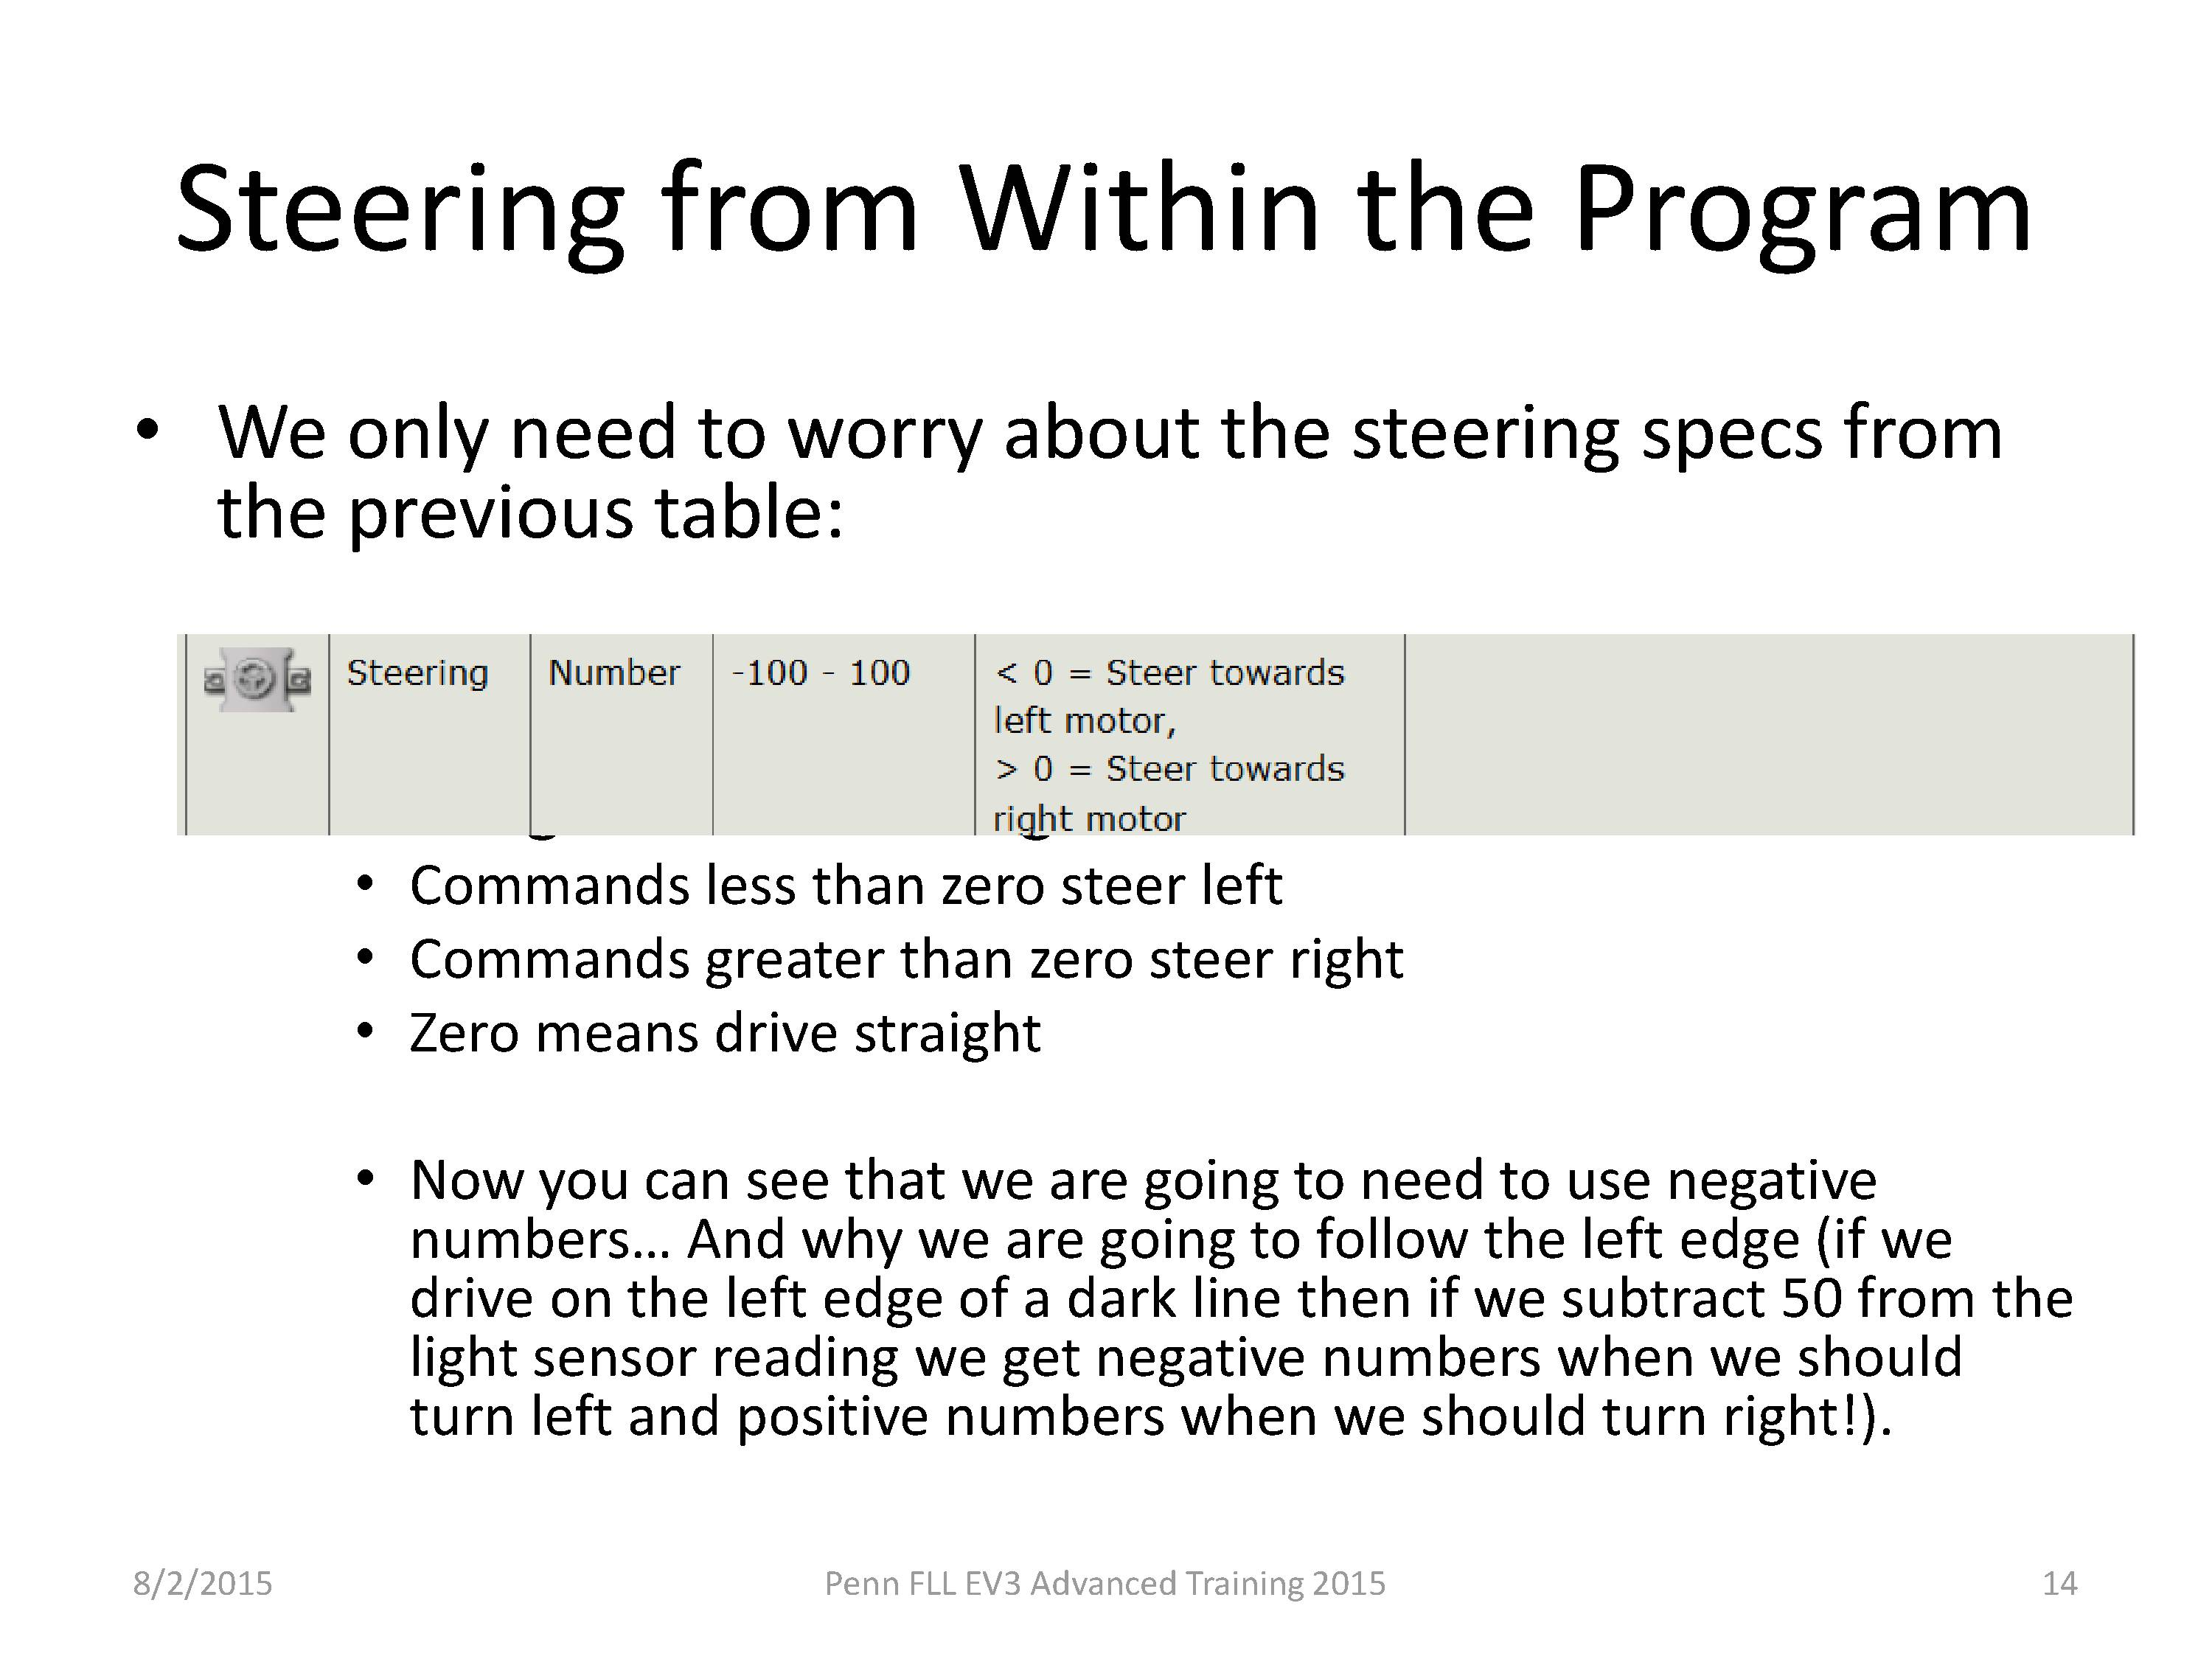
\includegraphics[scale=0.4]{ev3advanced2015/file-page14}
%\caption{lion!!}
\end{figure}
\end{frame}


\begin{frame}
%\frametitle{Pictures}
\begin{figure}
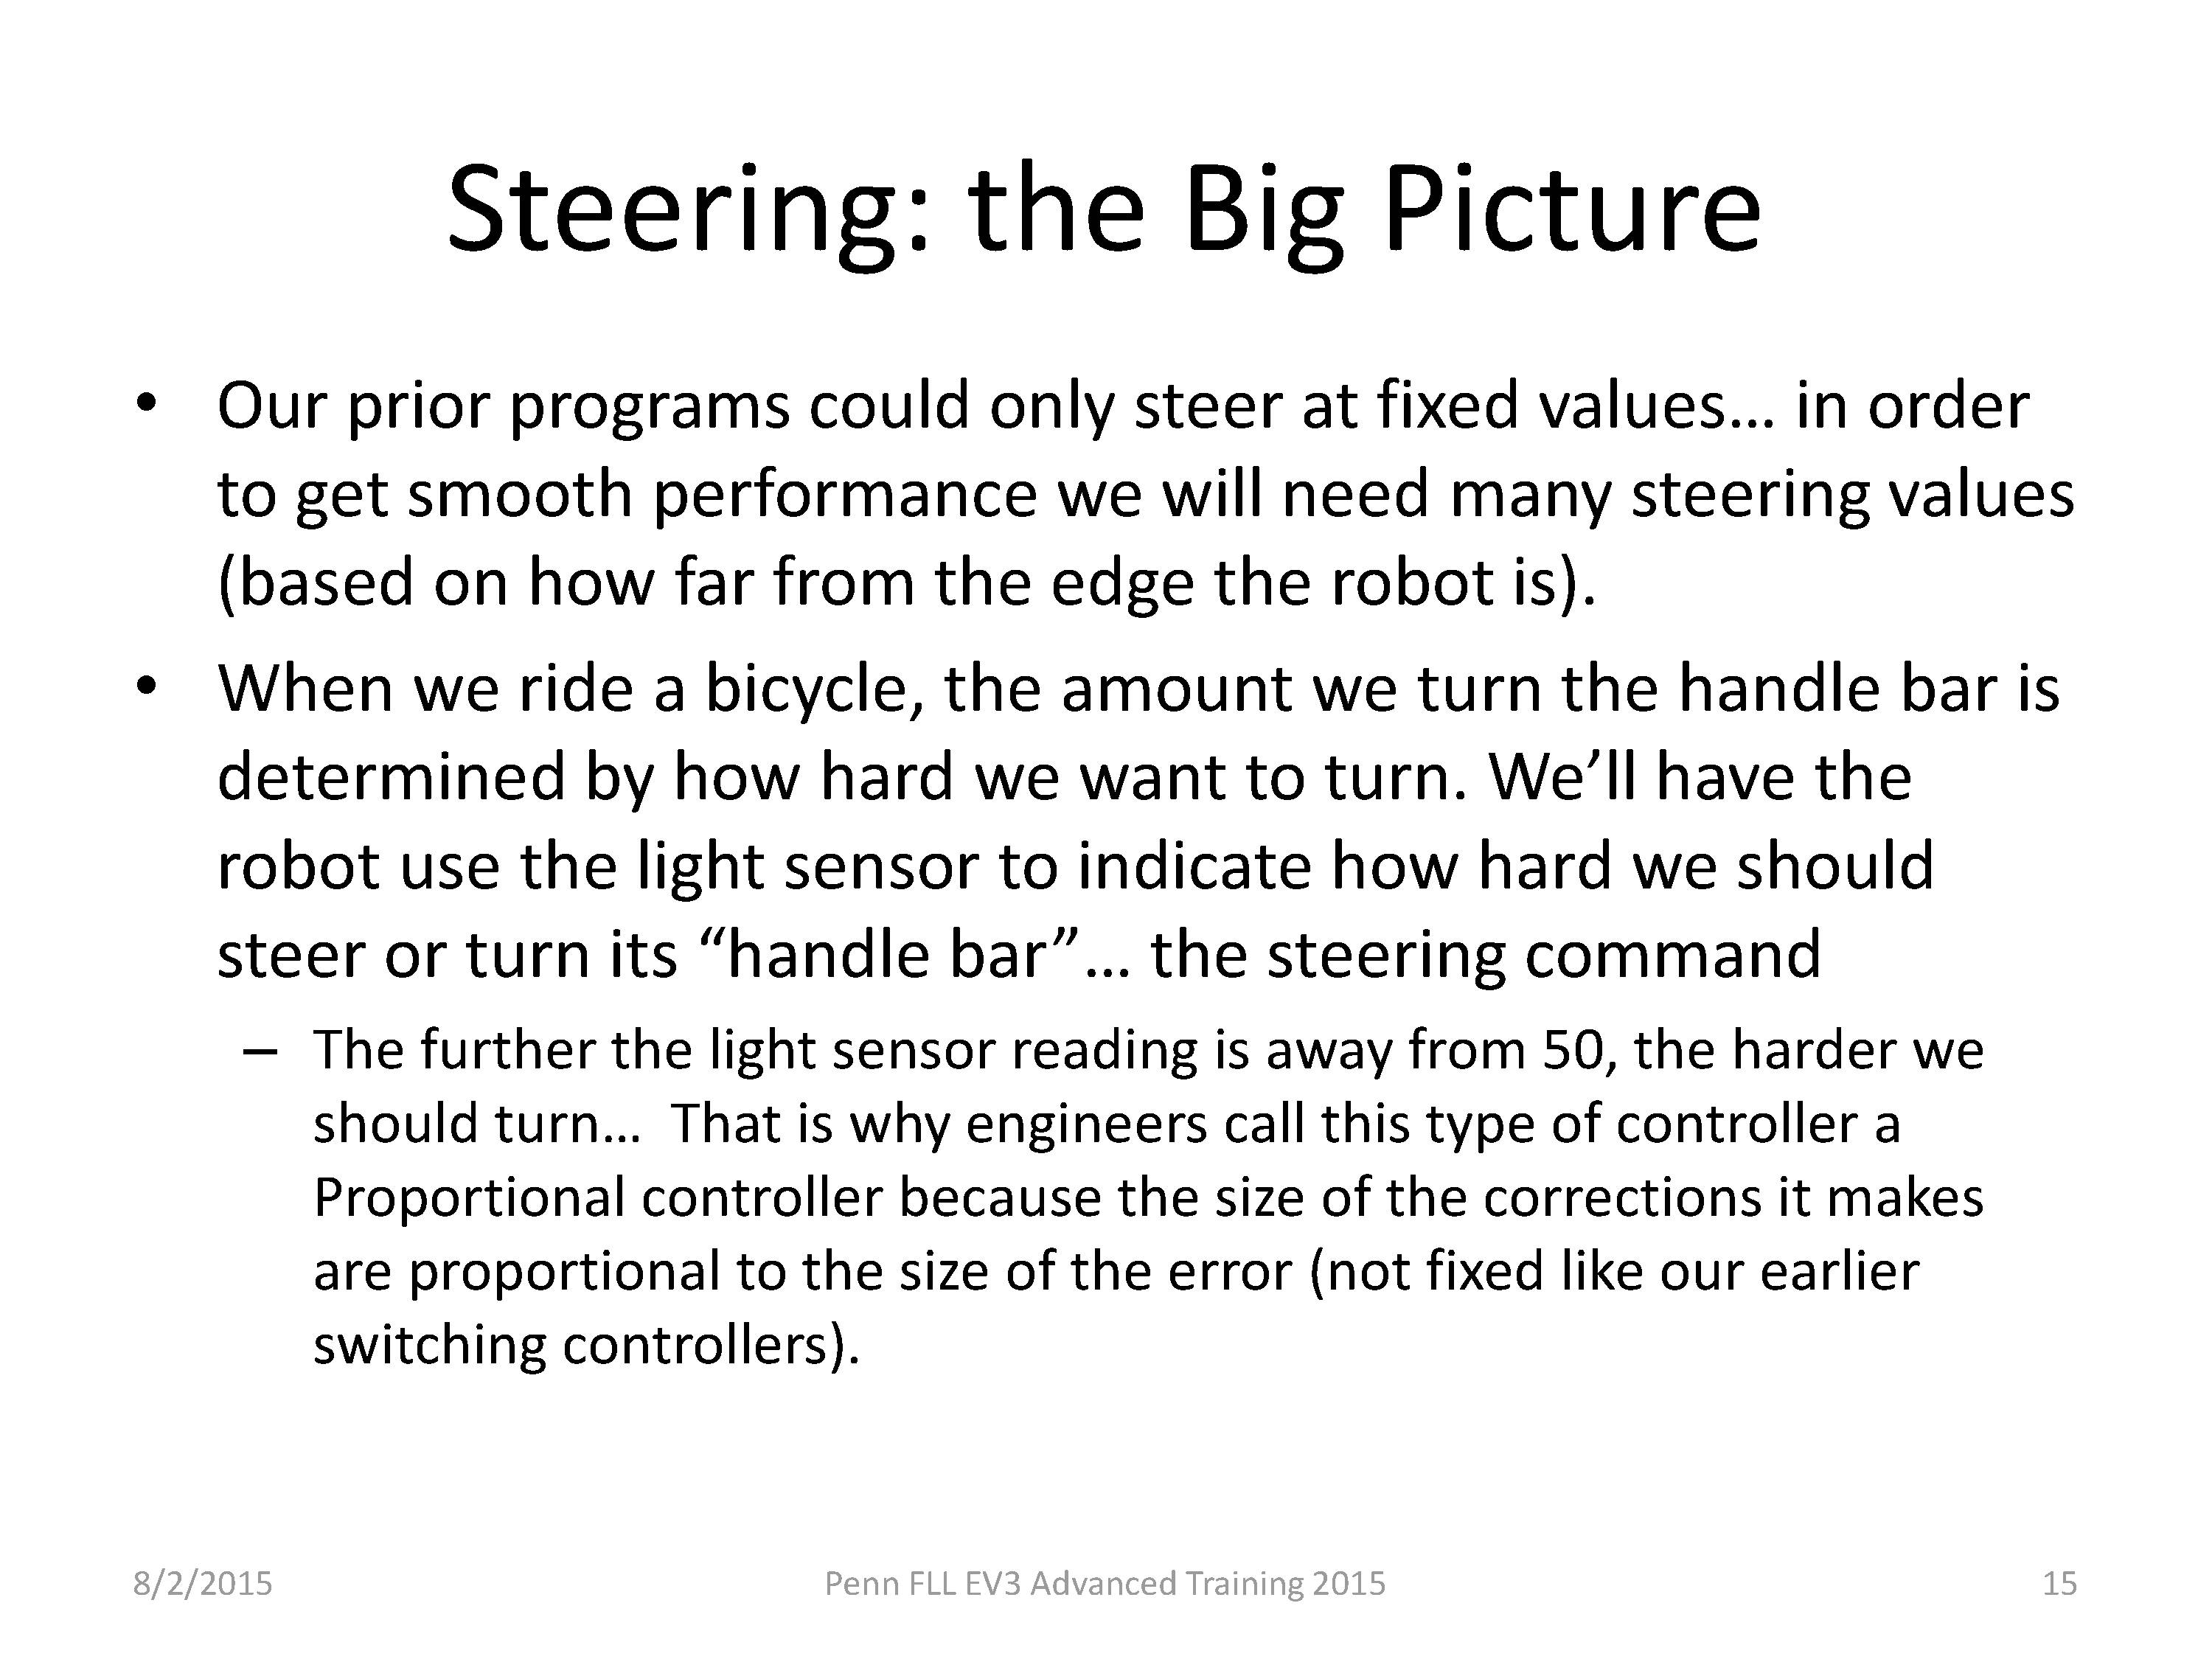
\includegraphics[scale=0.4]{ev3advanced2015/file-page15}
%\caption{lion!!}
\end{figure}
\end{frame}


\begin{frame}
%\frametitle{Pictures}
\begin{figure}
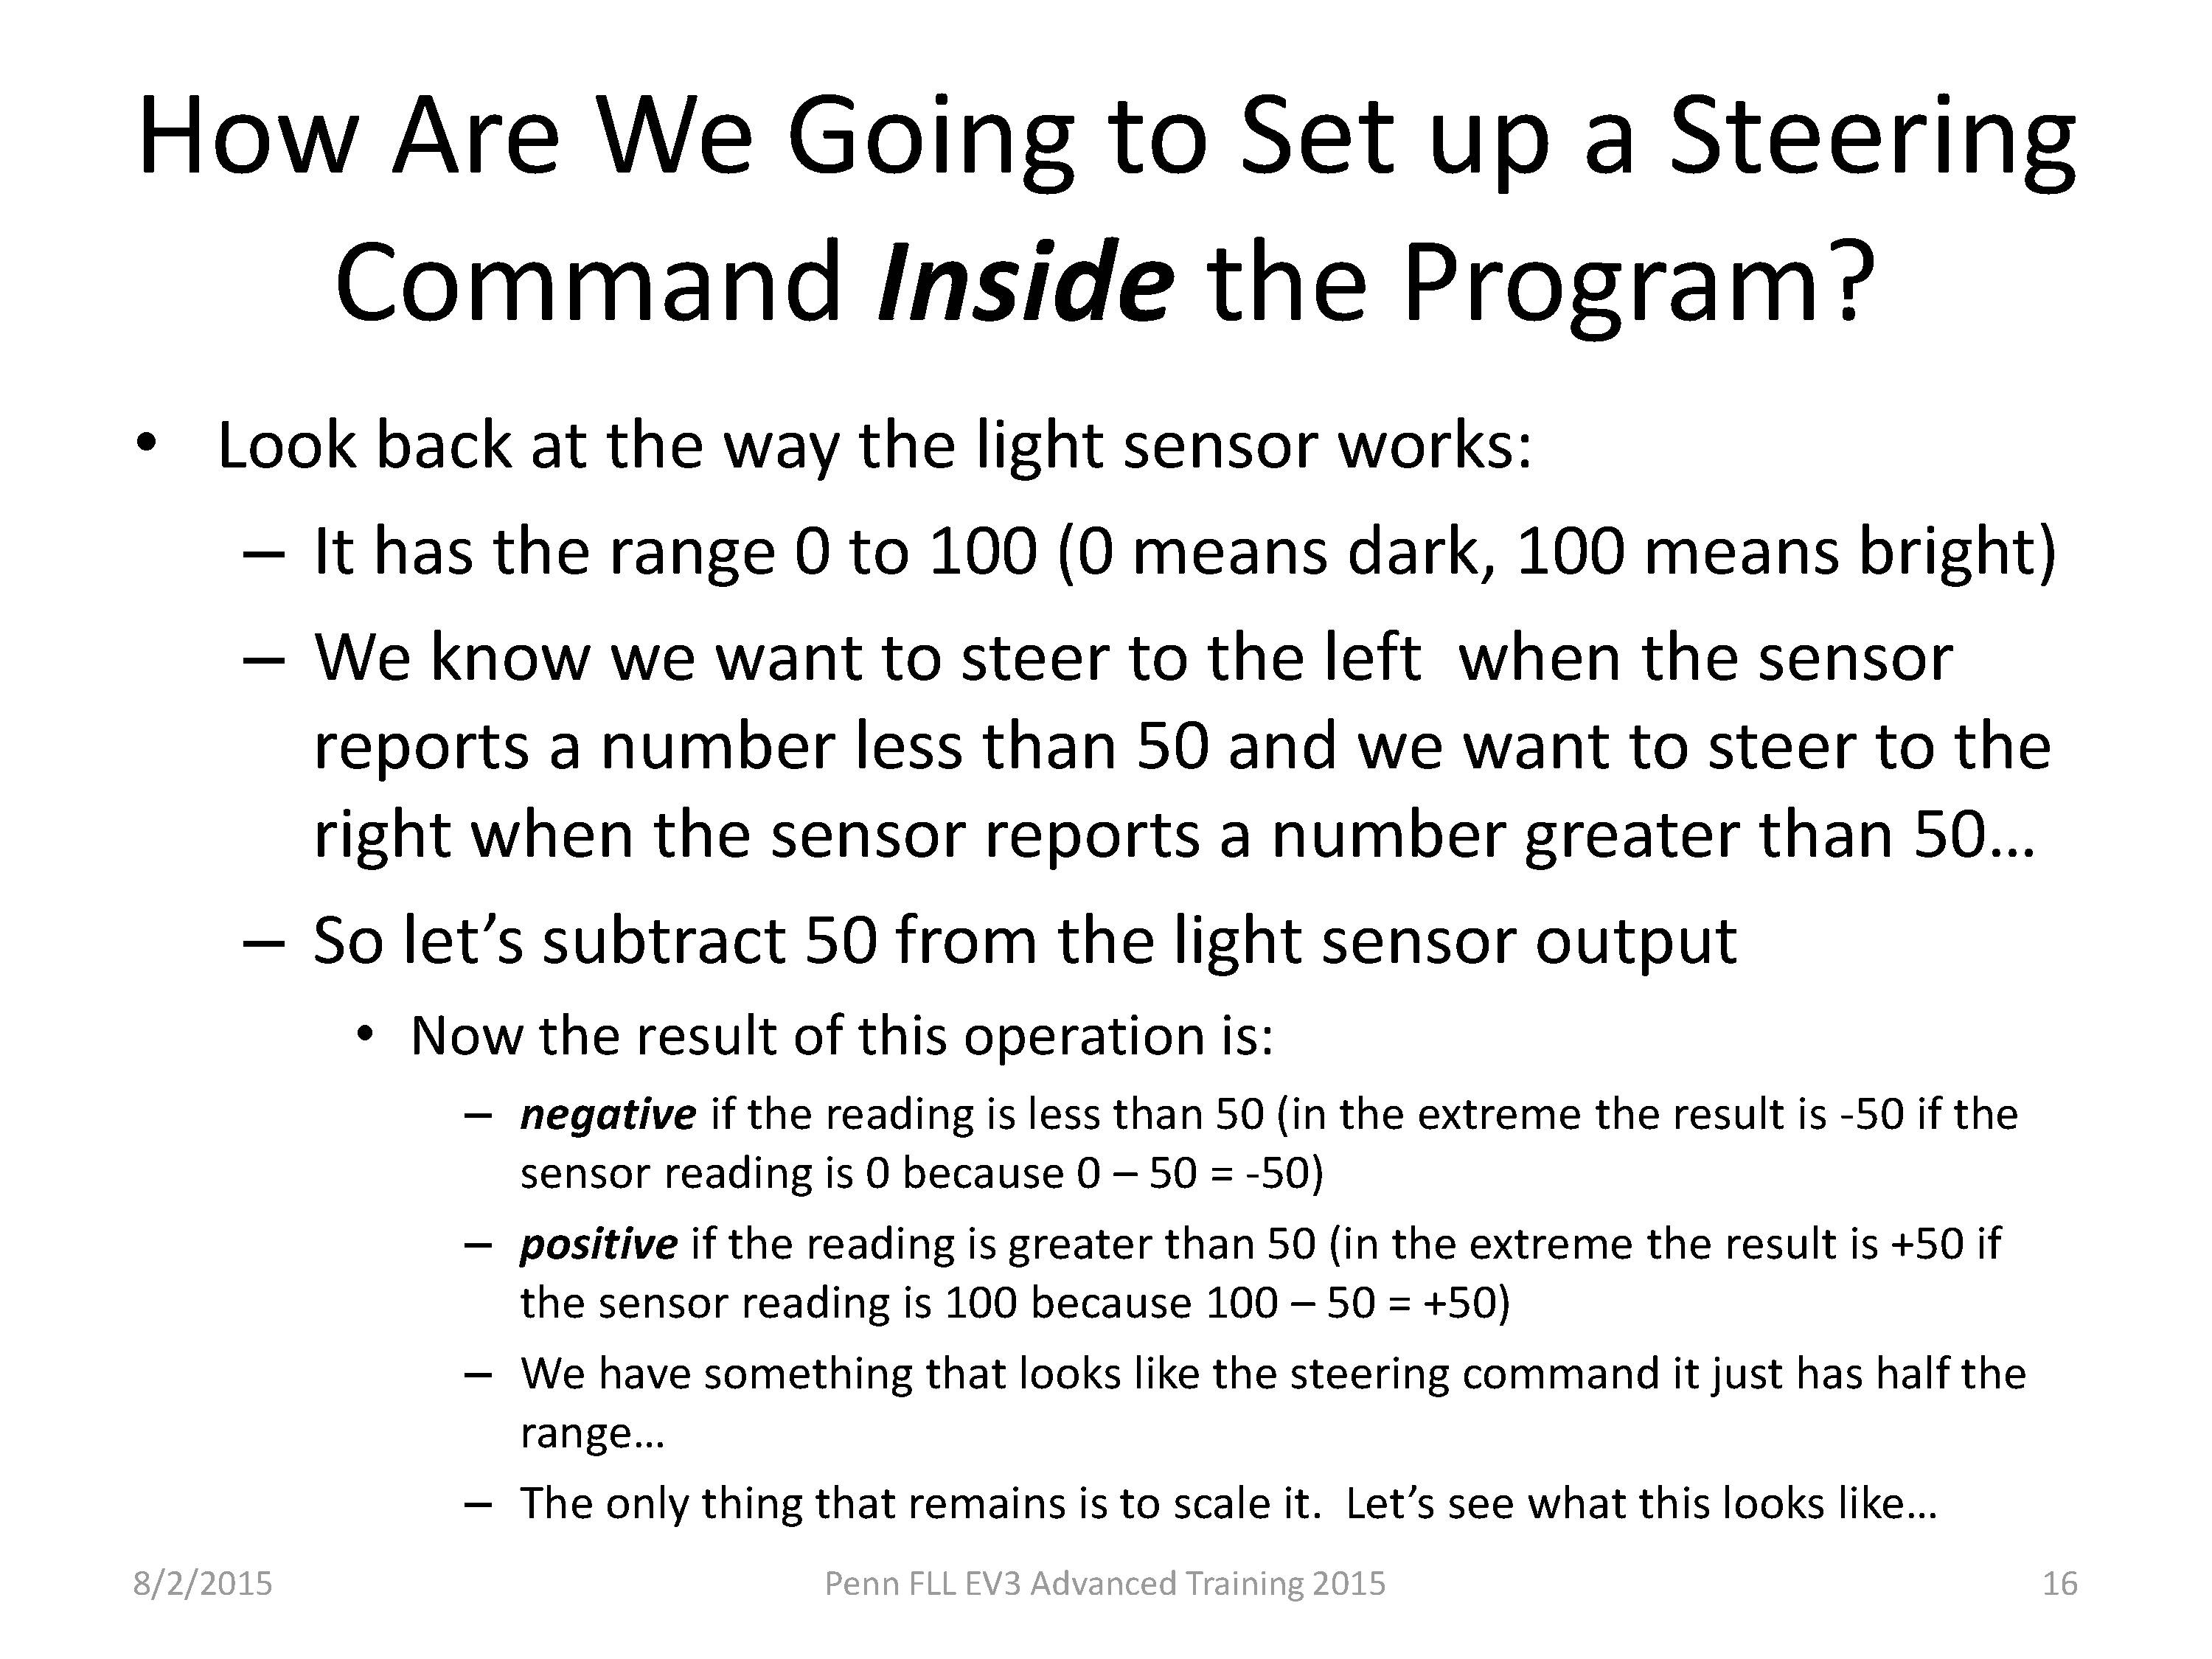
\includegraphics[scale=0.4]{ev3advanced2015/file-page16}
%\caption{lion!!}
\end{figure}
\end{frame}


\begin{frame}
%\frametitle{Pictures}
\begin{figure}
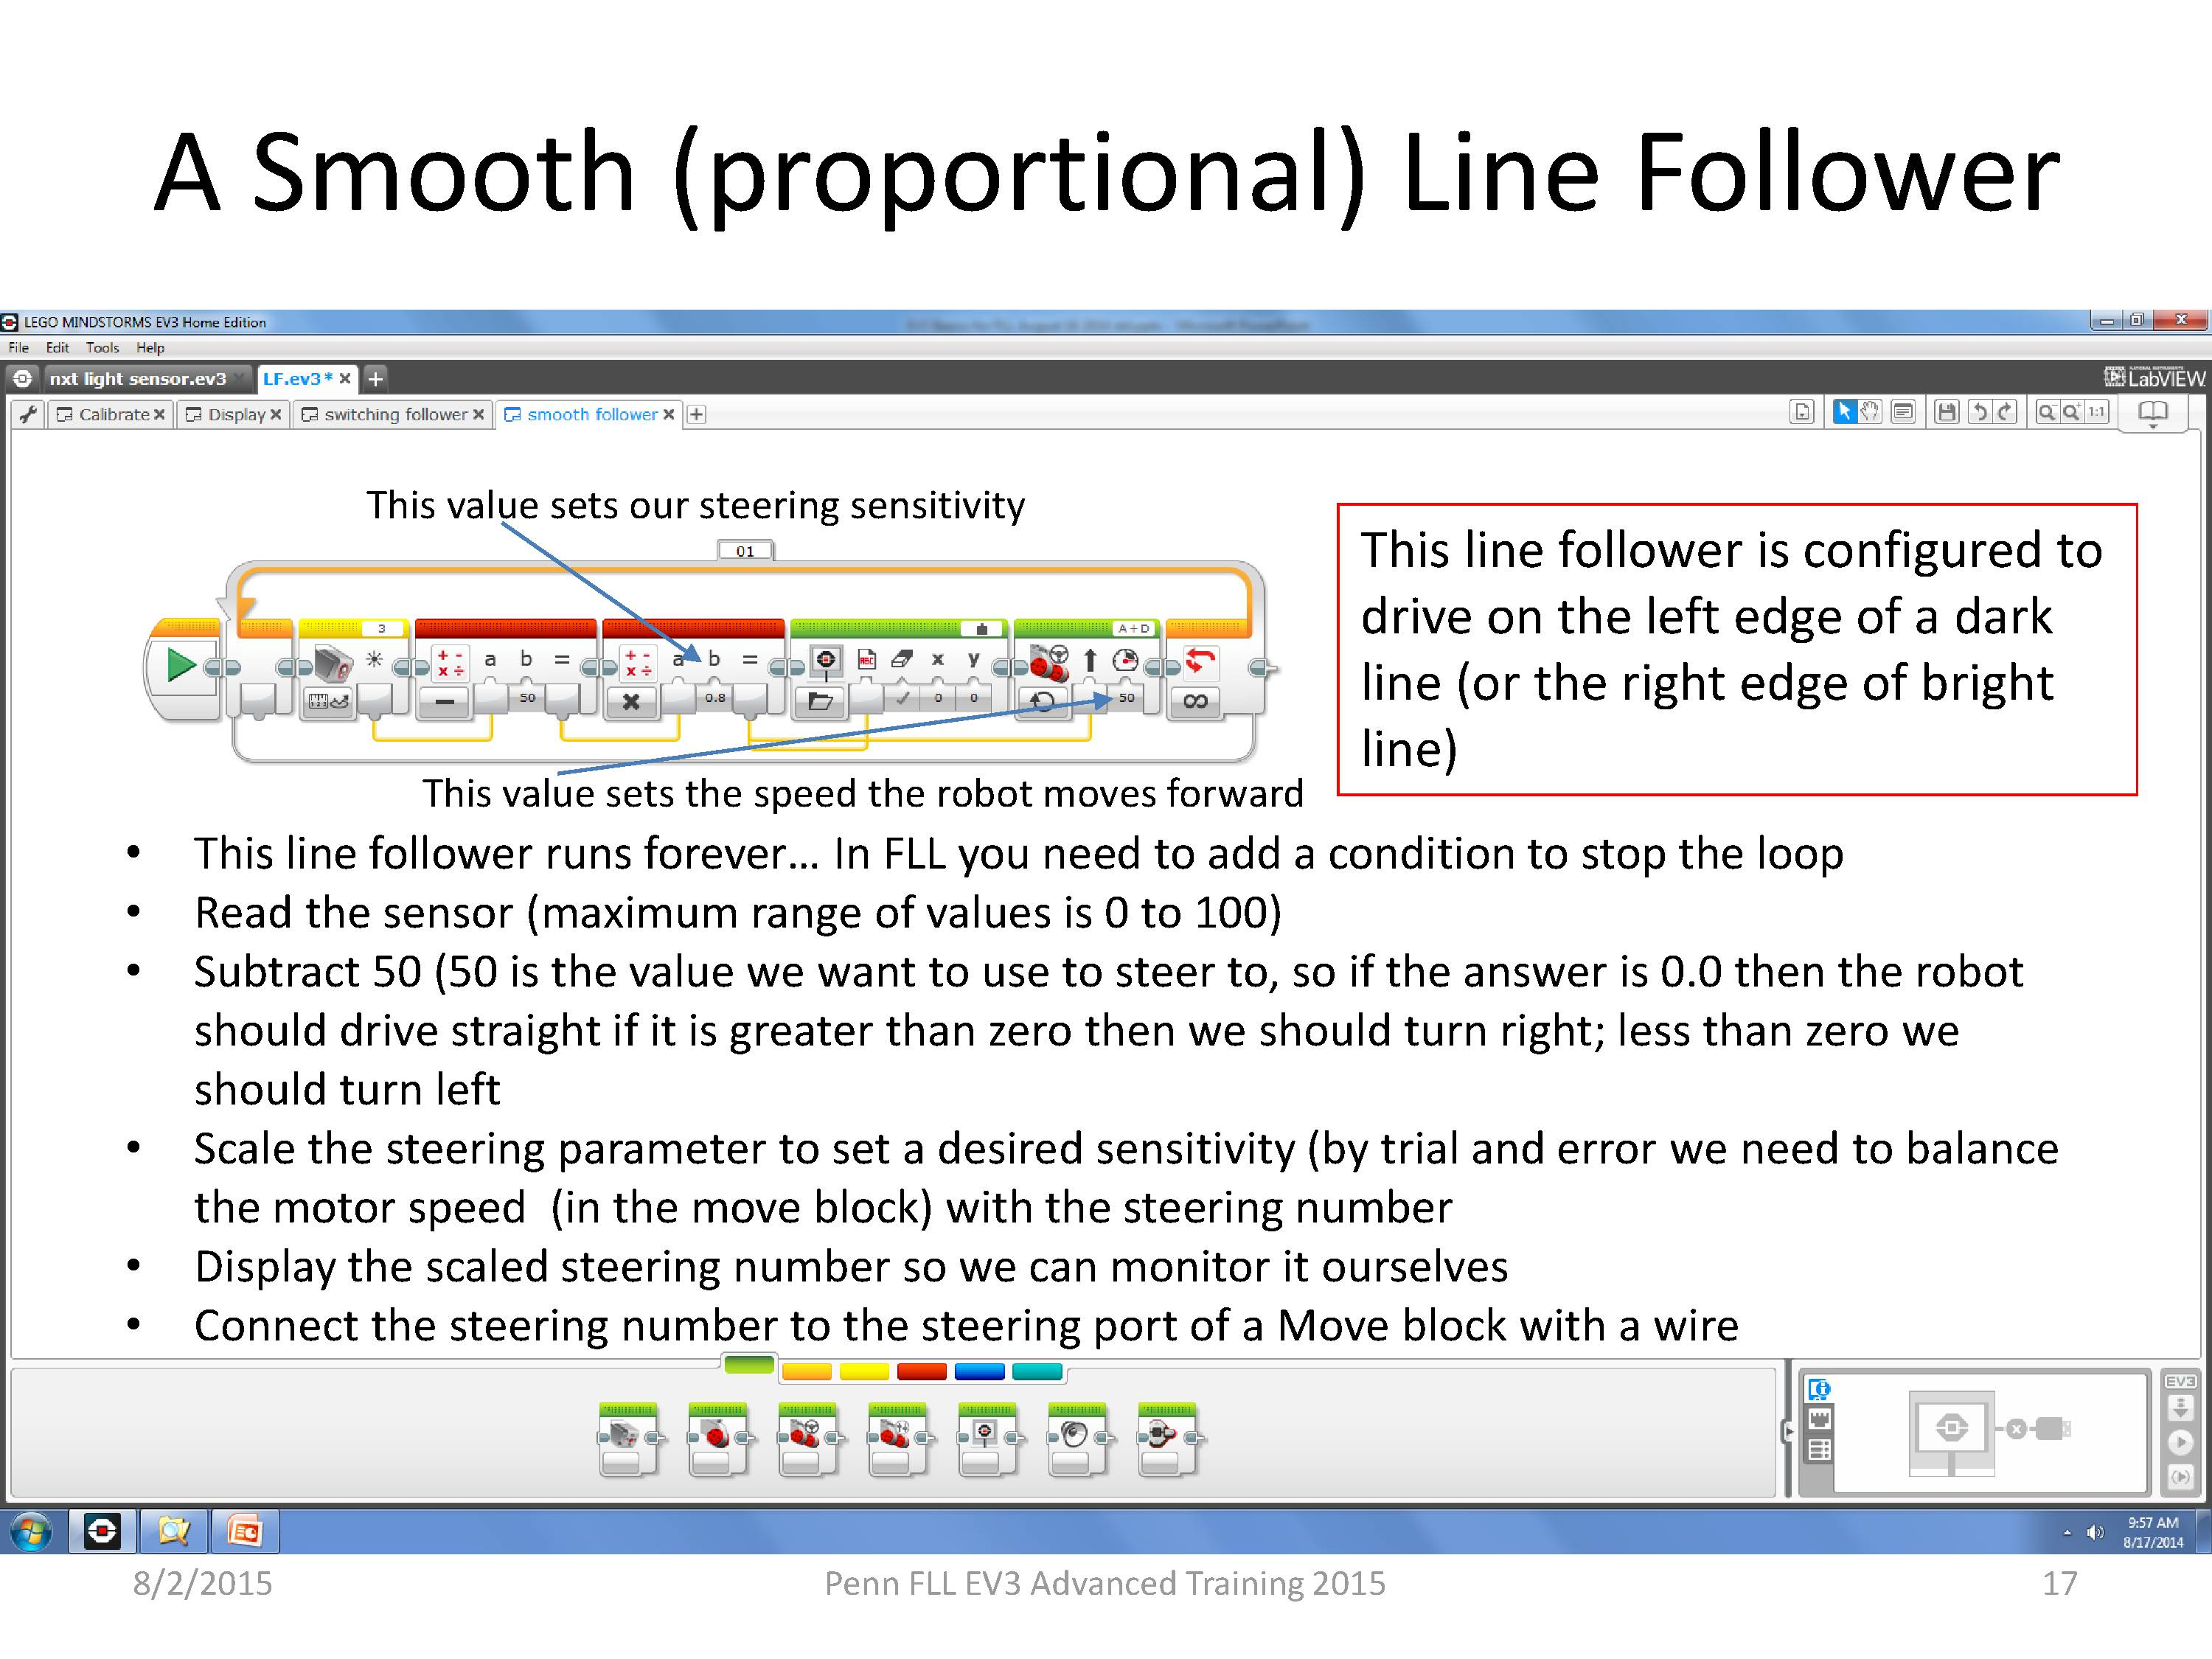
\includegraphics[scale=0.4]{ev3advanced2015/file-page17}
%\caption{lion!!}
\end{figure}
\end{frame}


\begin{frame}
%\frametitle{Pictures}
\begin{figure}
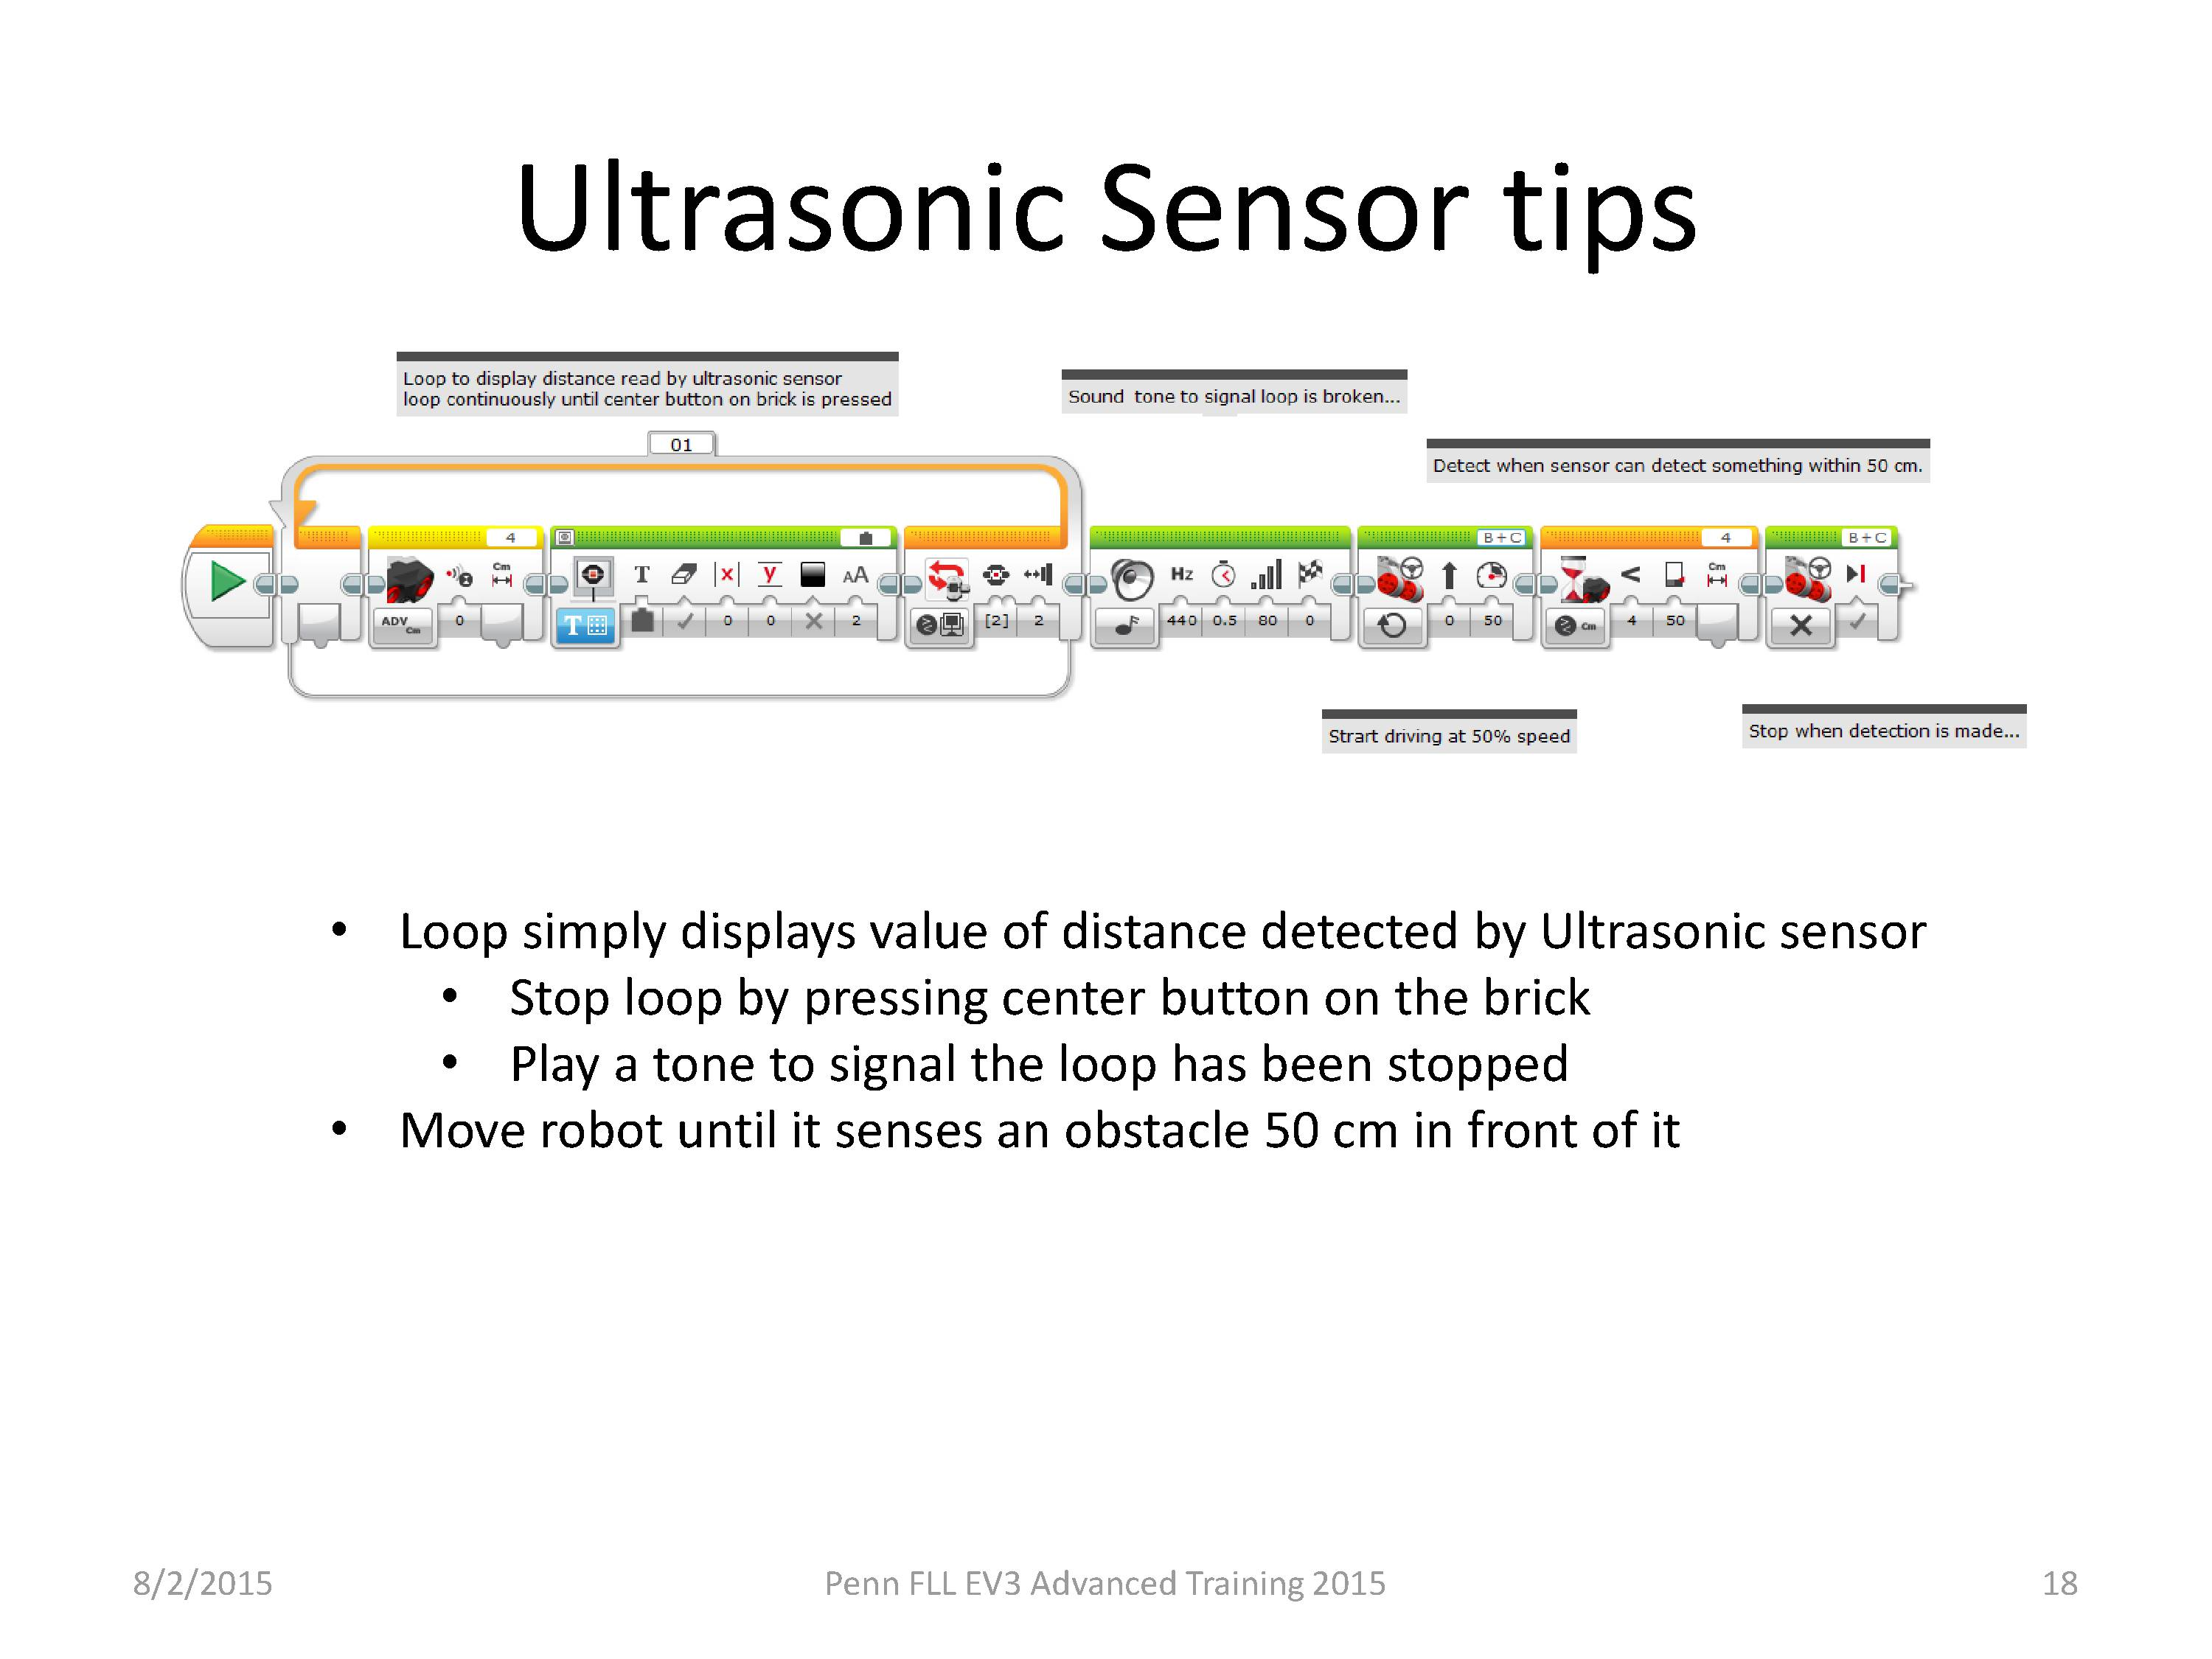
\includegraphics[scale=0.4]{ev3advanced2015/file-page18}
%\caption{lion!!}
\end{figure}
\end{frame}


\begin{frame}
%\frametitle{Pictures}
\begin{figure}
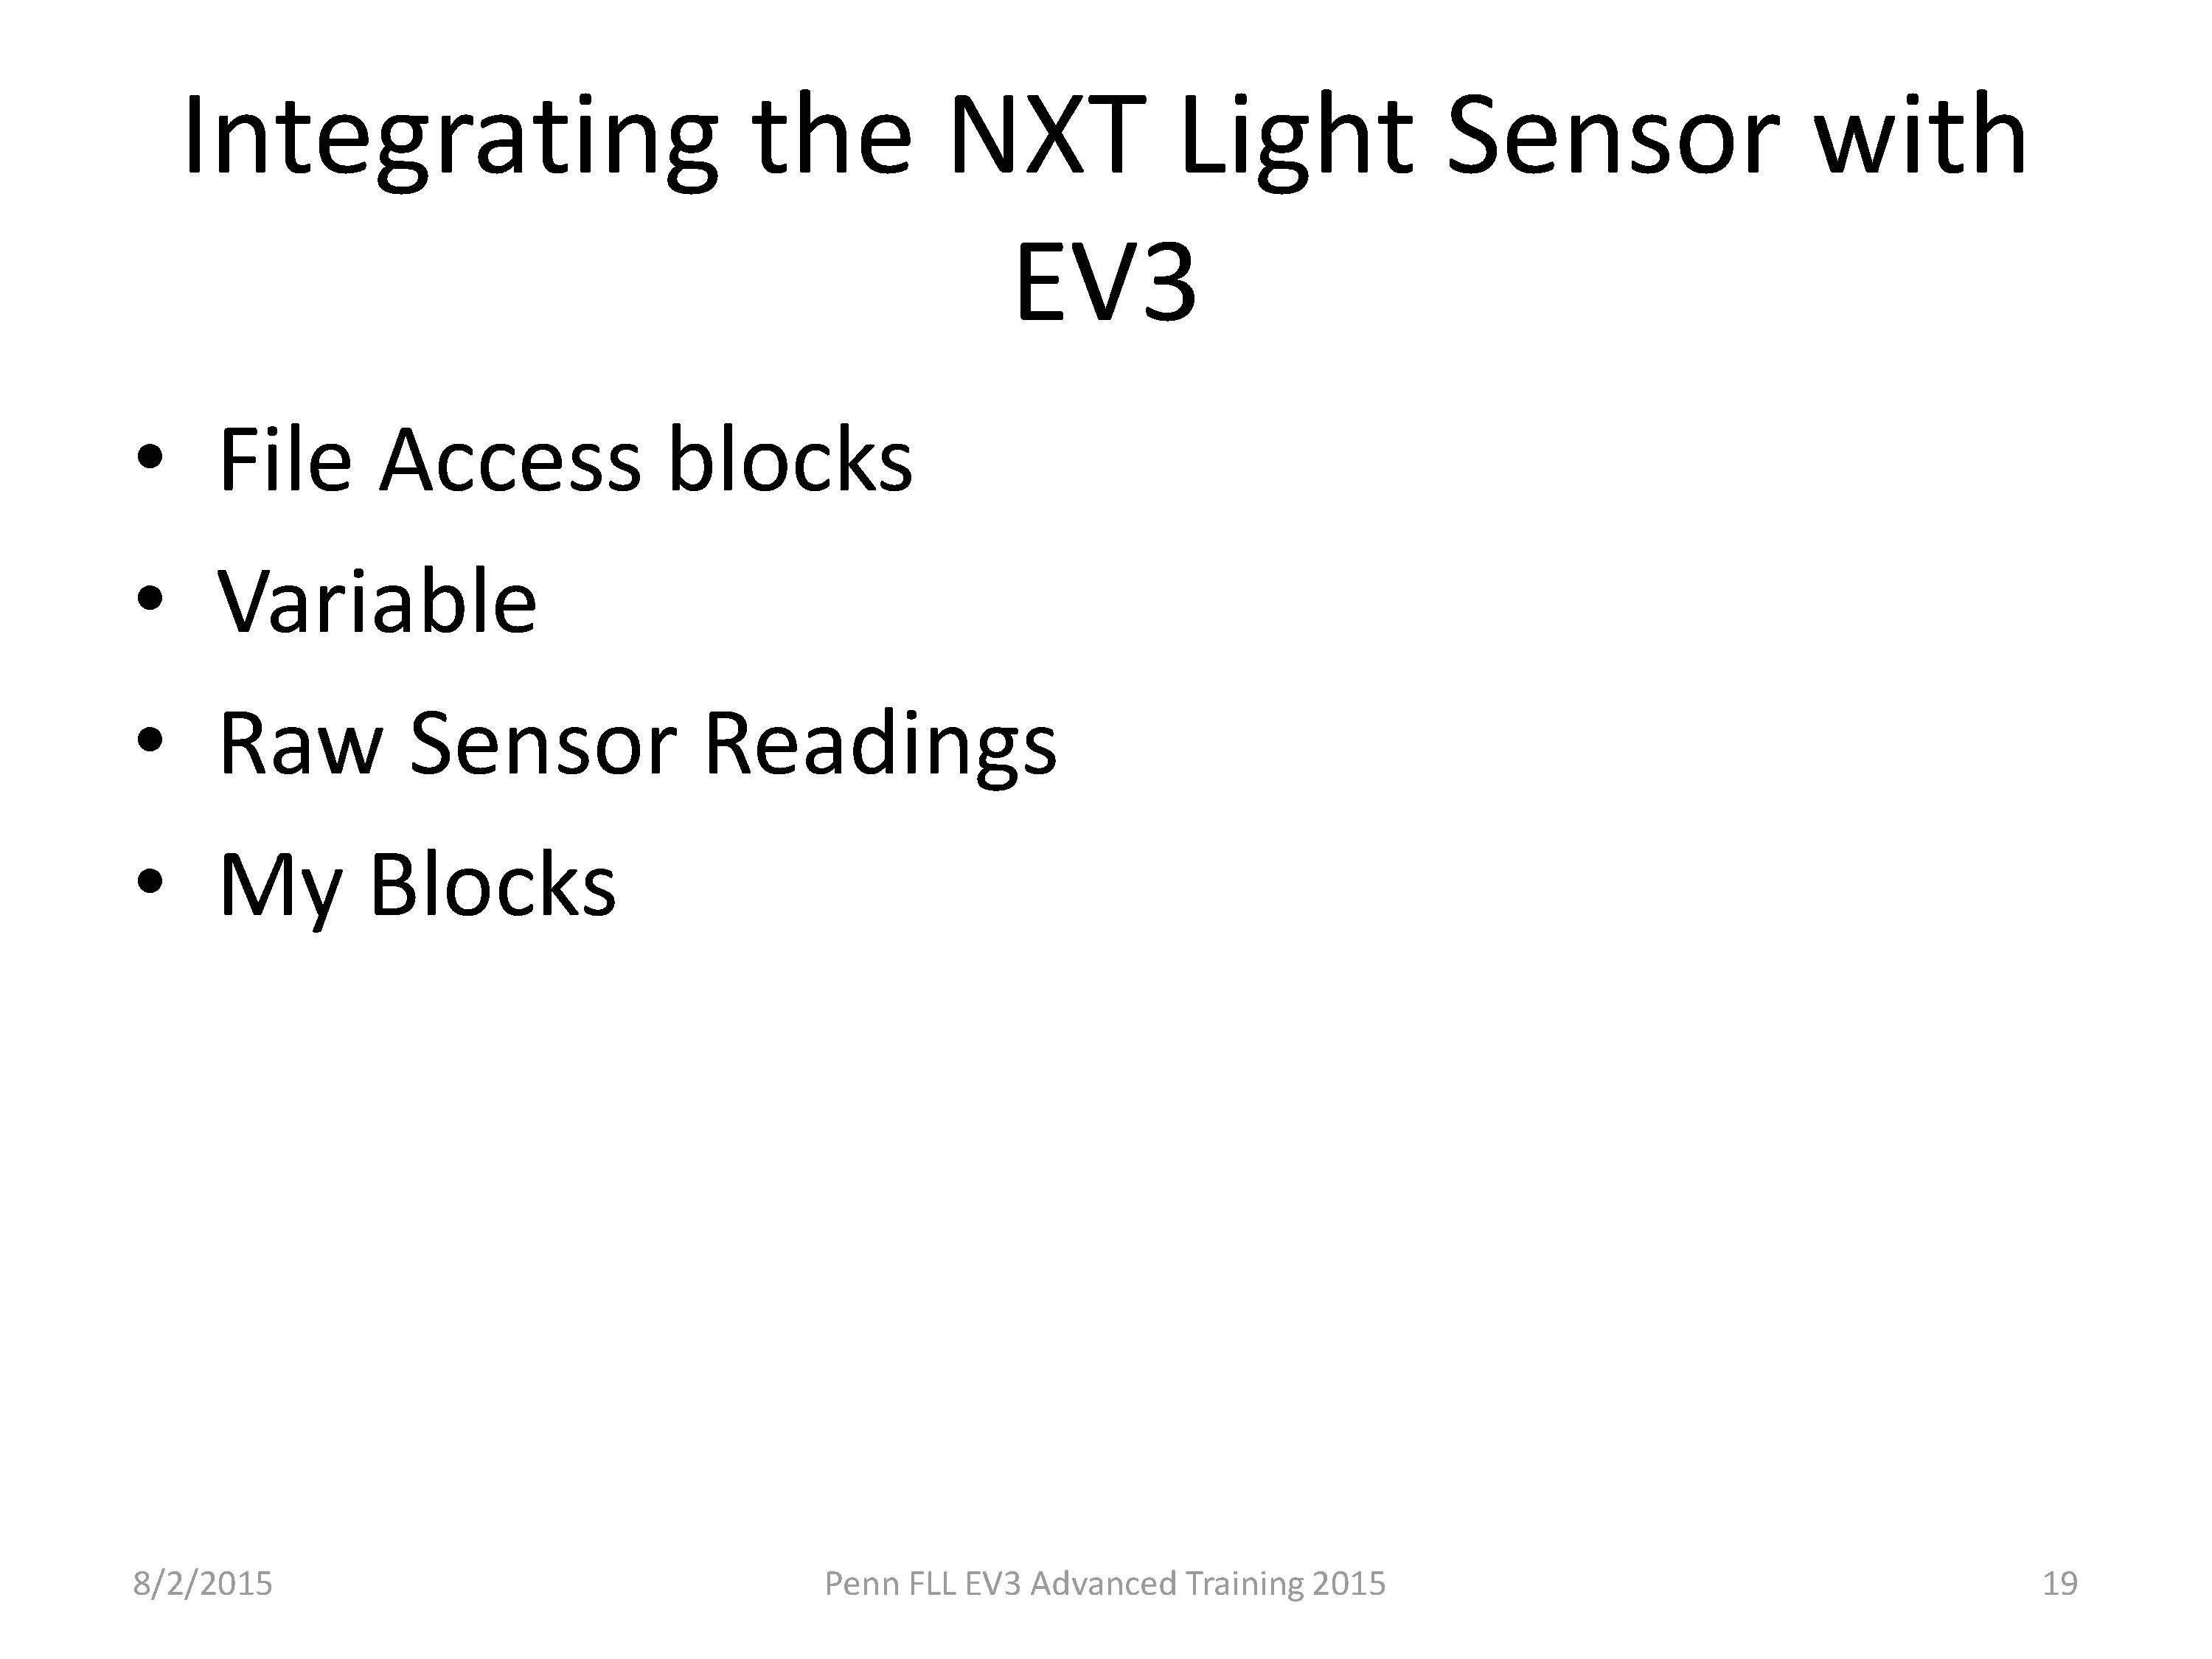
\includegraphics[scale=0.4]{ev3advanced2015/file-page19}
%\caption{lion!!}
\end{figure}
\end{frame}


\begin{frame}
%\frametitle{Pictures}
\begin{figure}
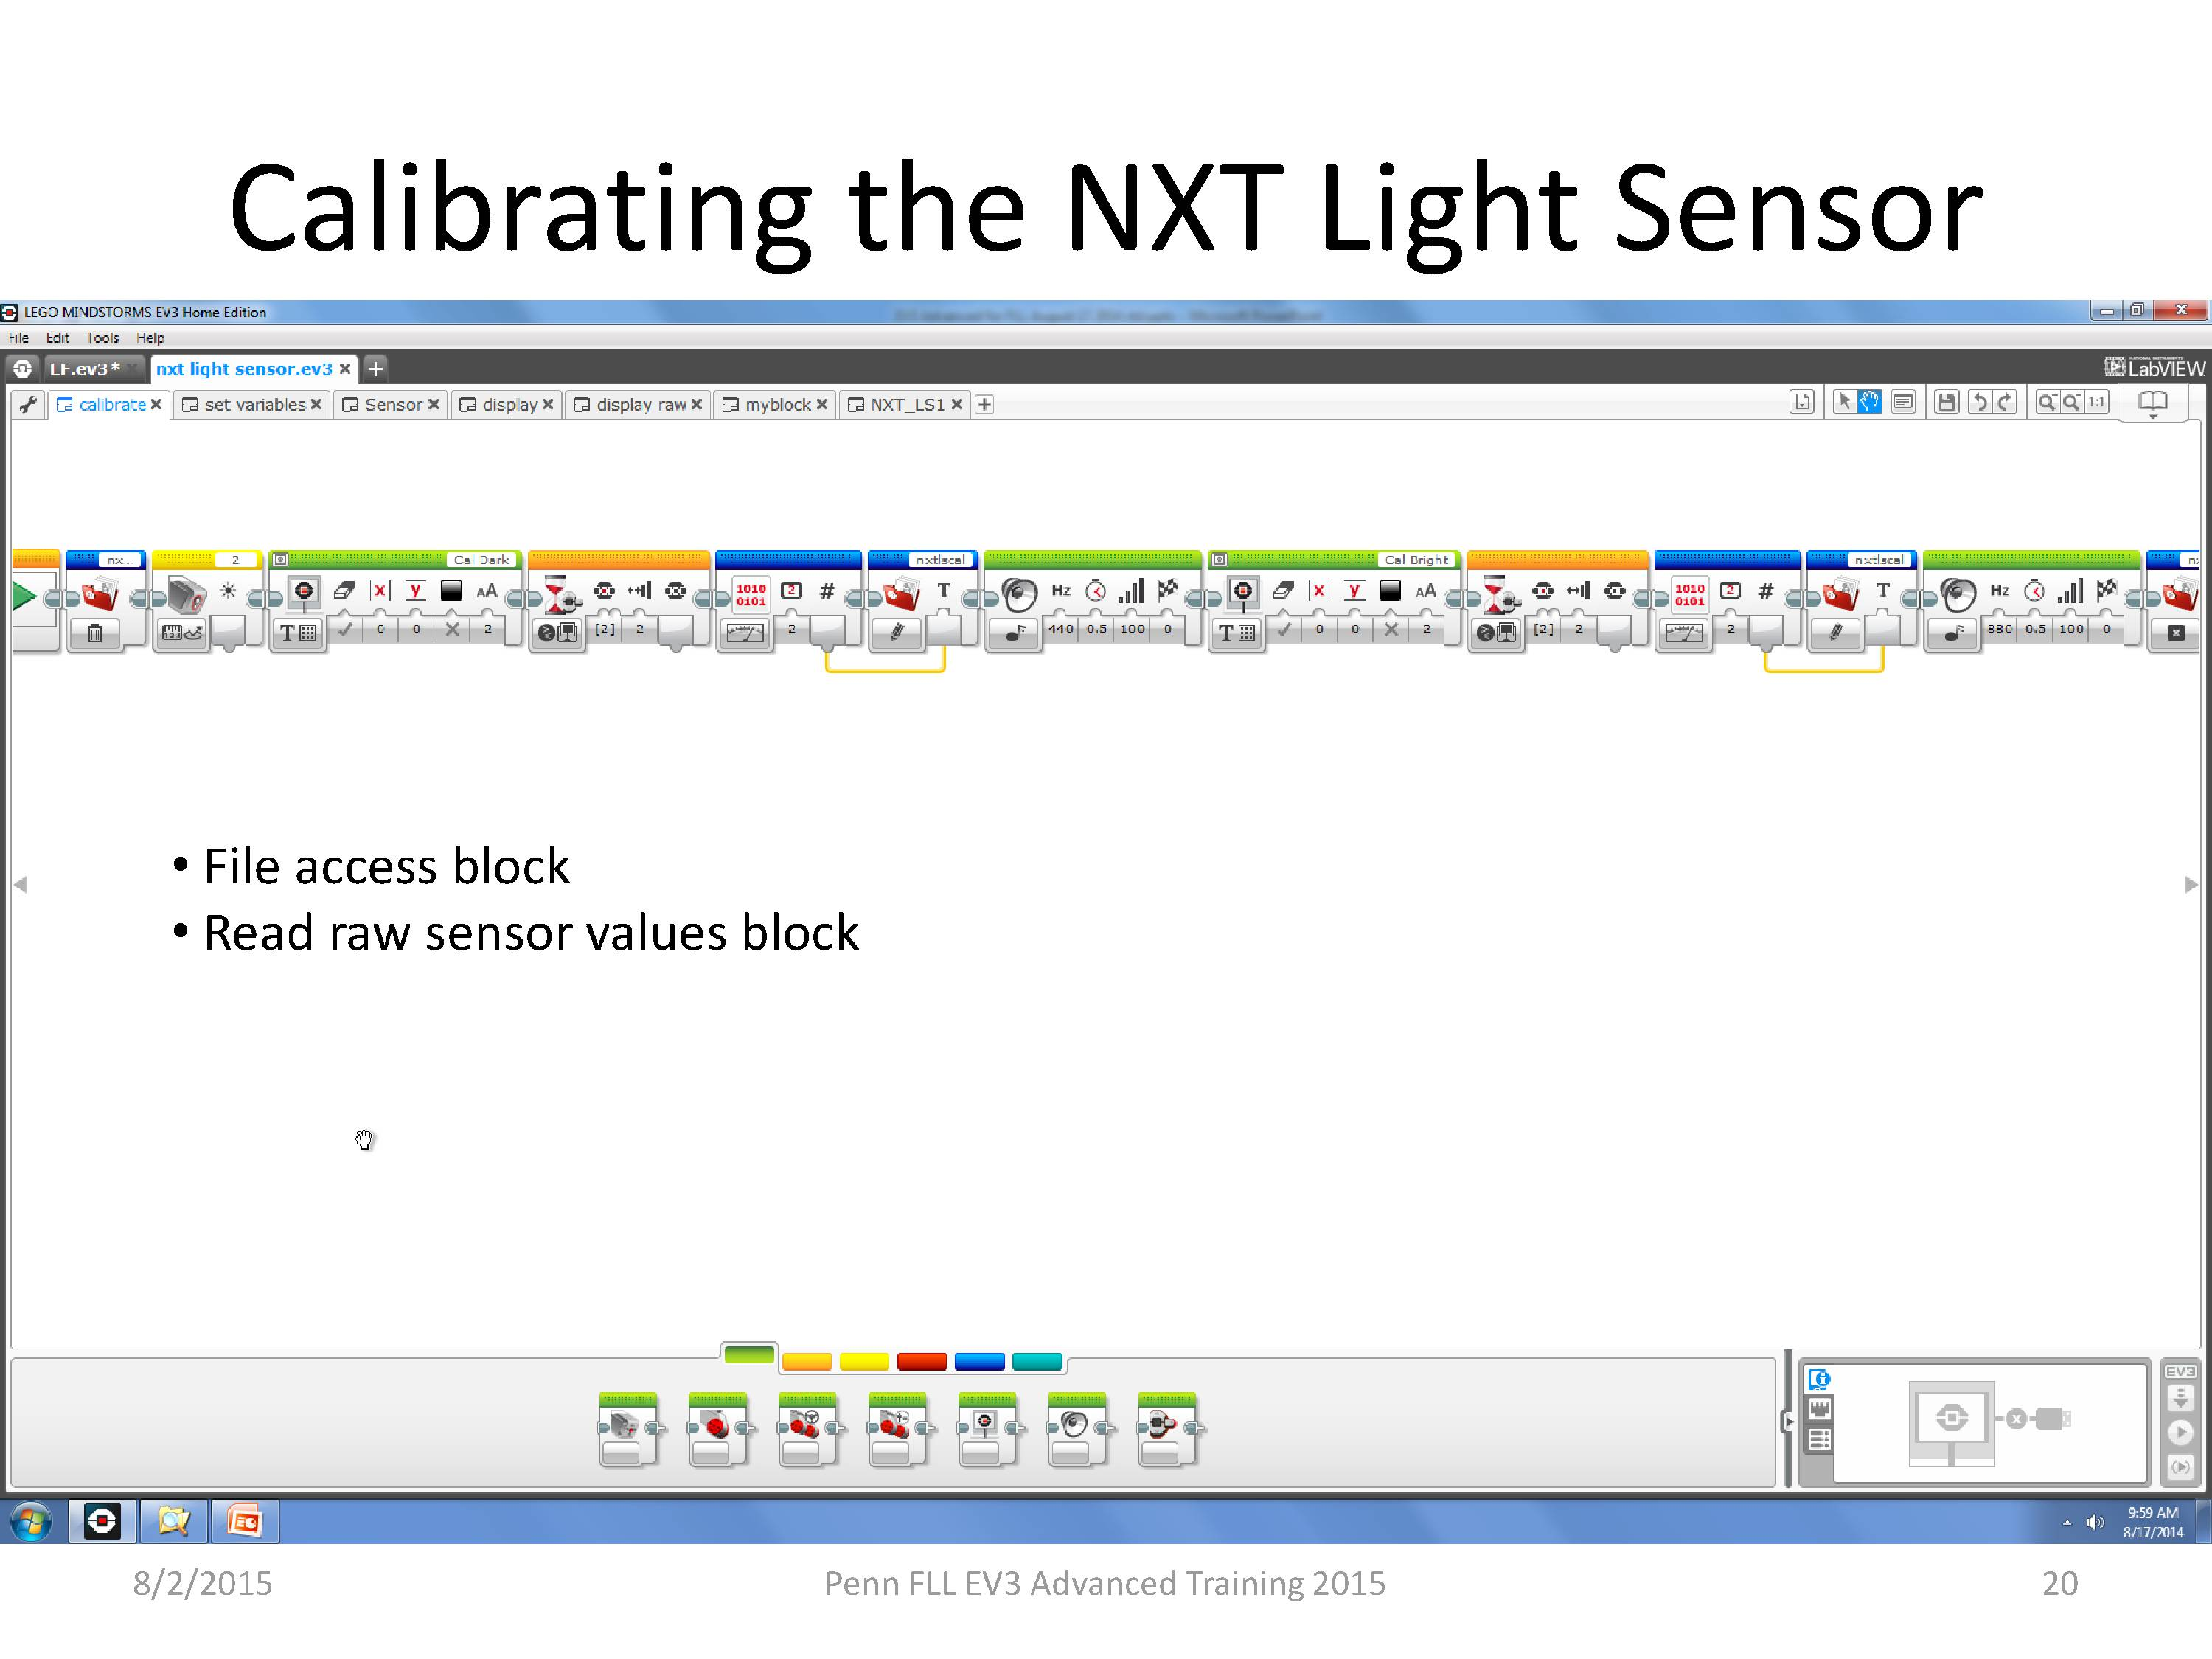
\includegraphics[scale=0.4]{ev3advanced2015/file-page20}
%\caption{lion!!}
\end{figure}
\end{frame}


\begin{frame}
%\frametitle{Pictures}
\begin{figure}
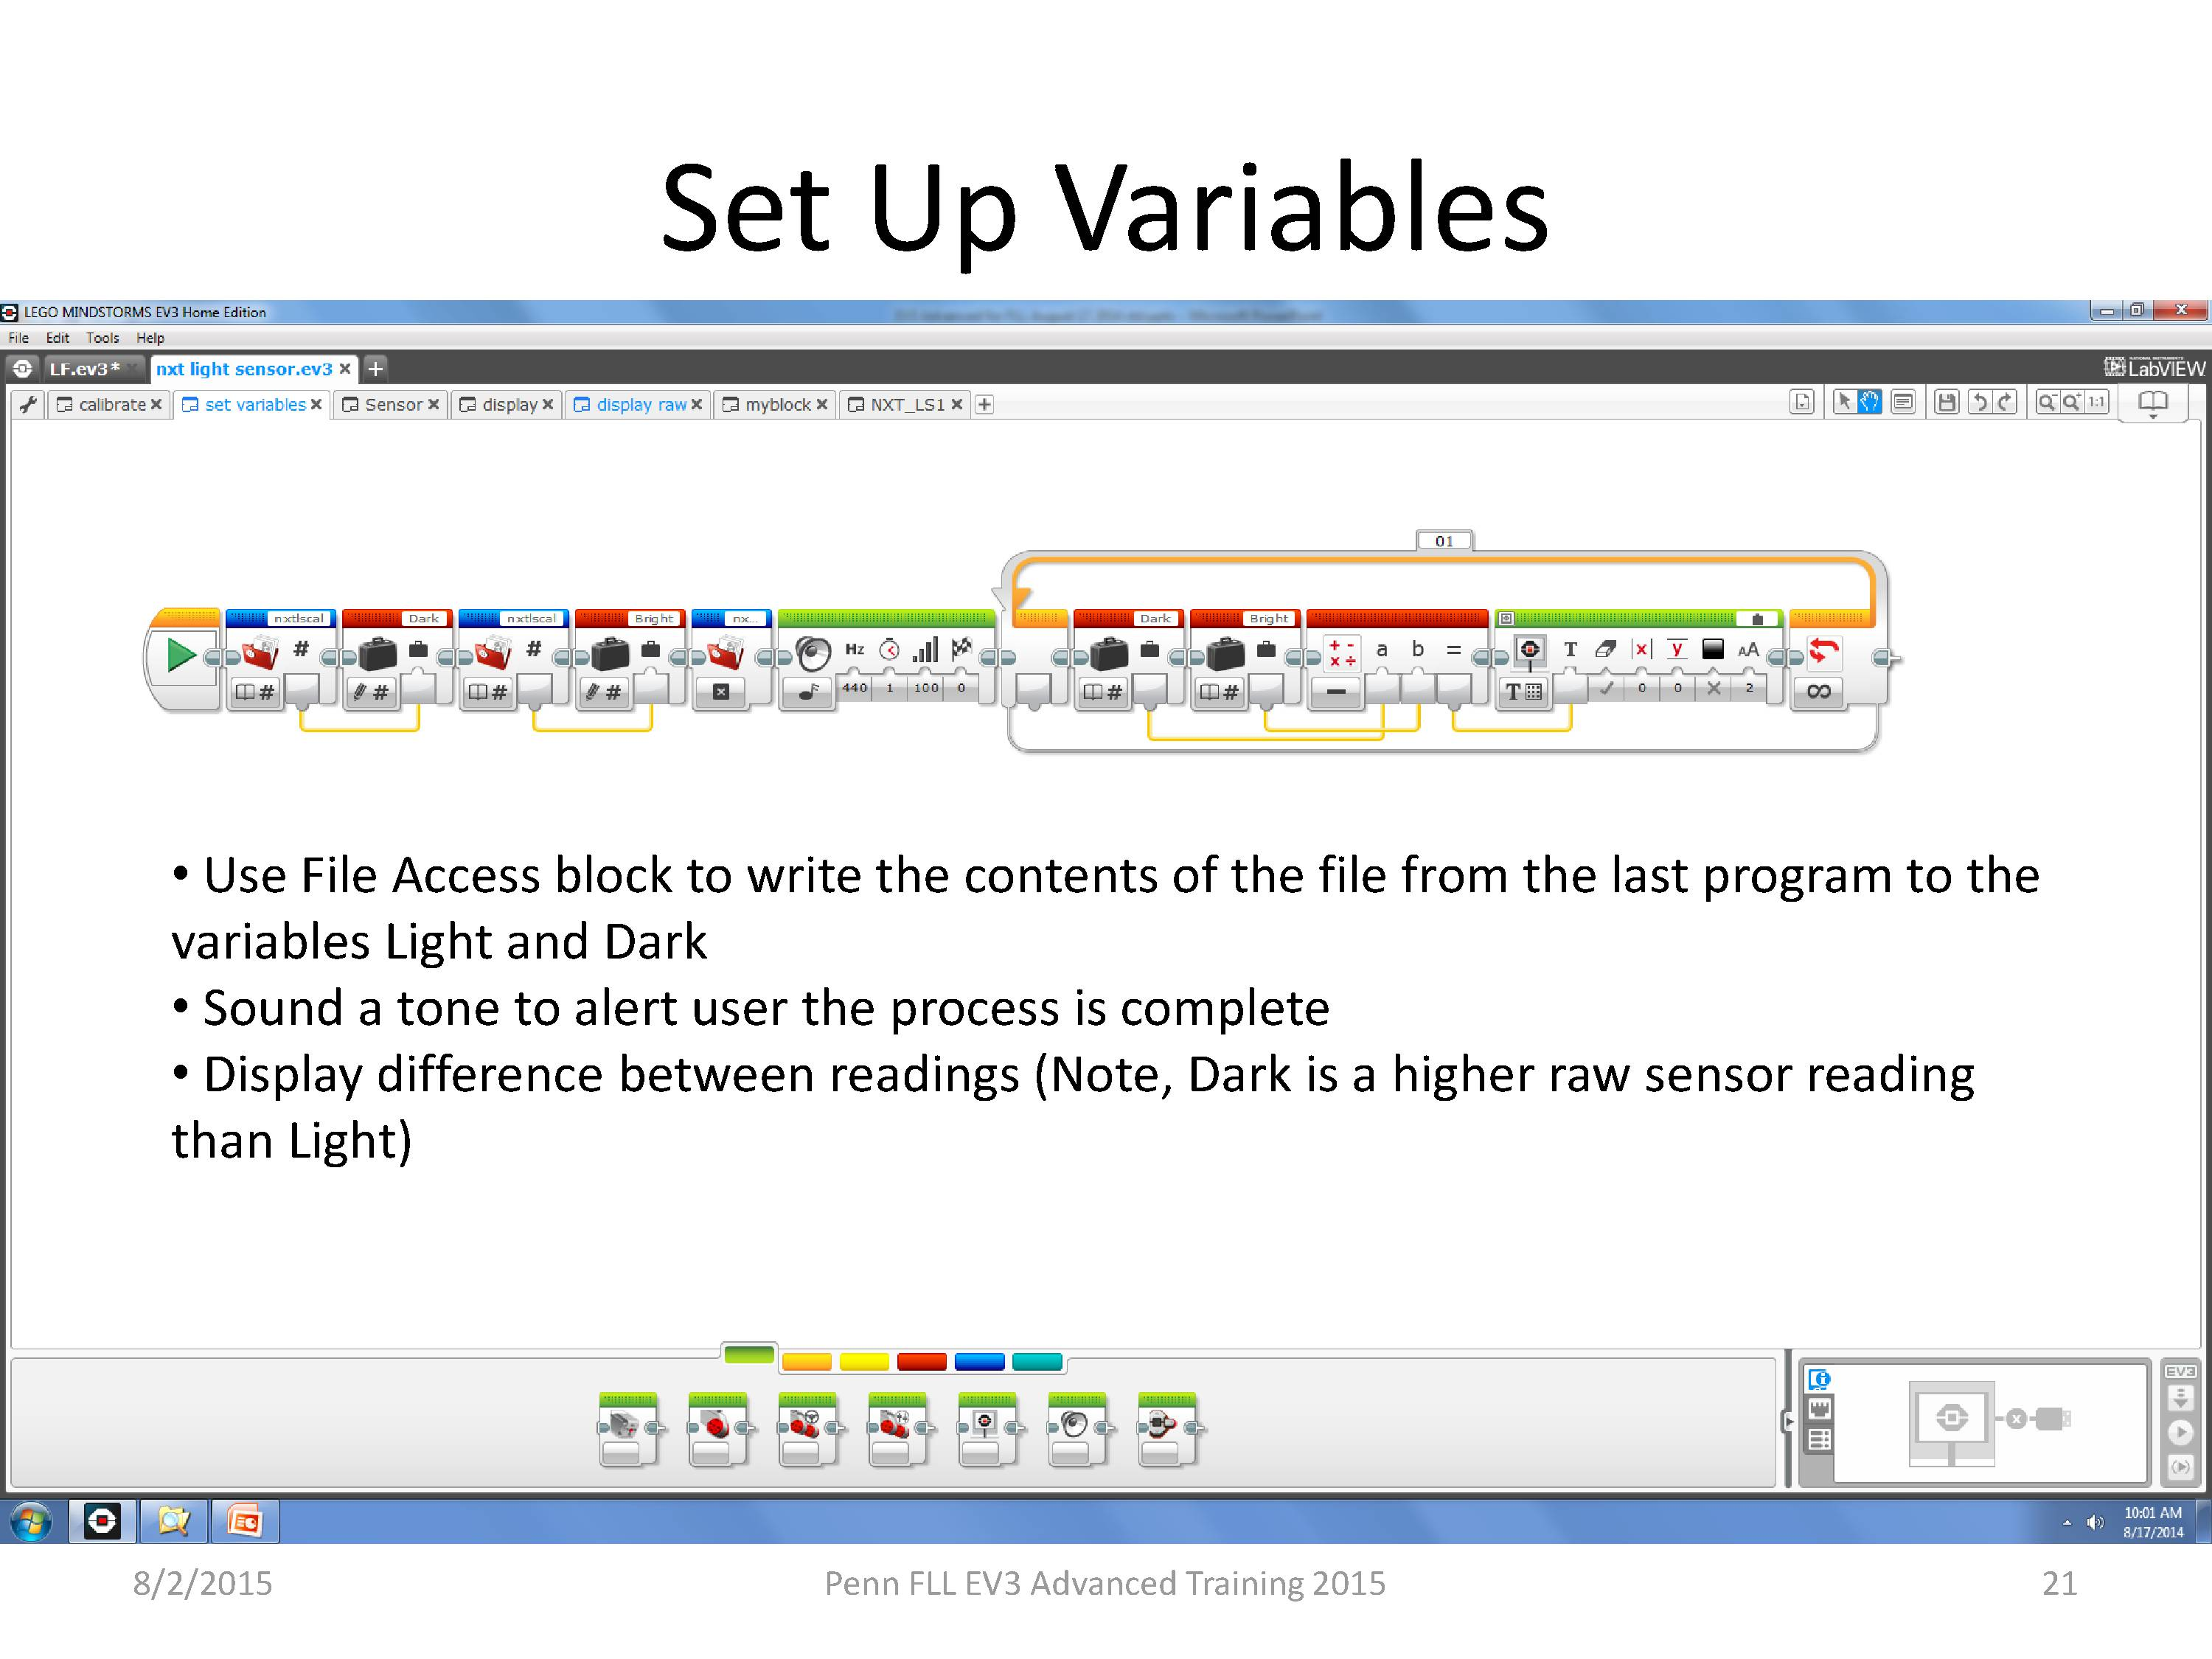
\includegraphics[scale=0.4]{ev3advanced2015/file-page21}
%\caption{lion!!}
\end{figure}
\end{frame}

\begin{frame}
%\frametitle{Pictures}
\begin{figure}
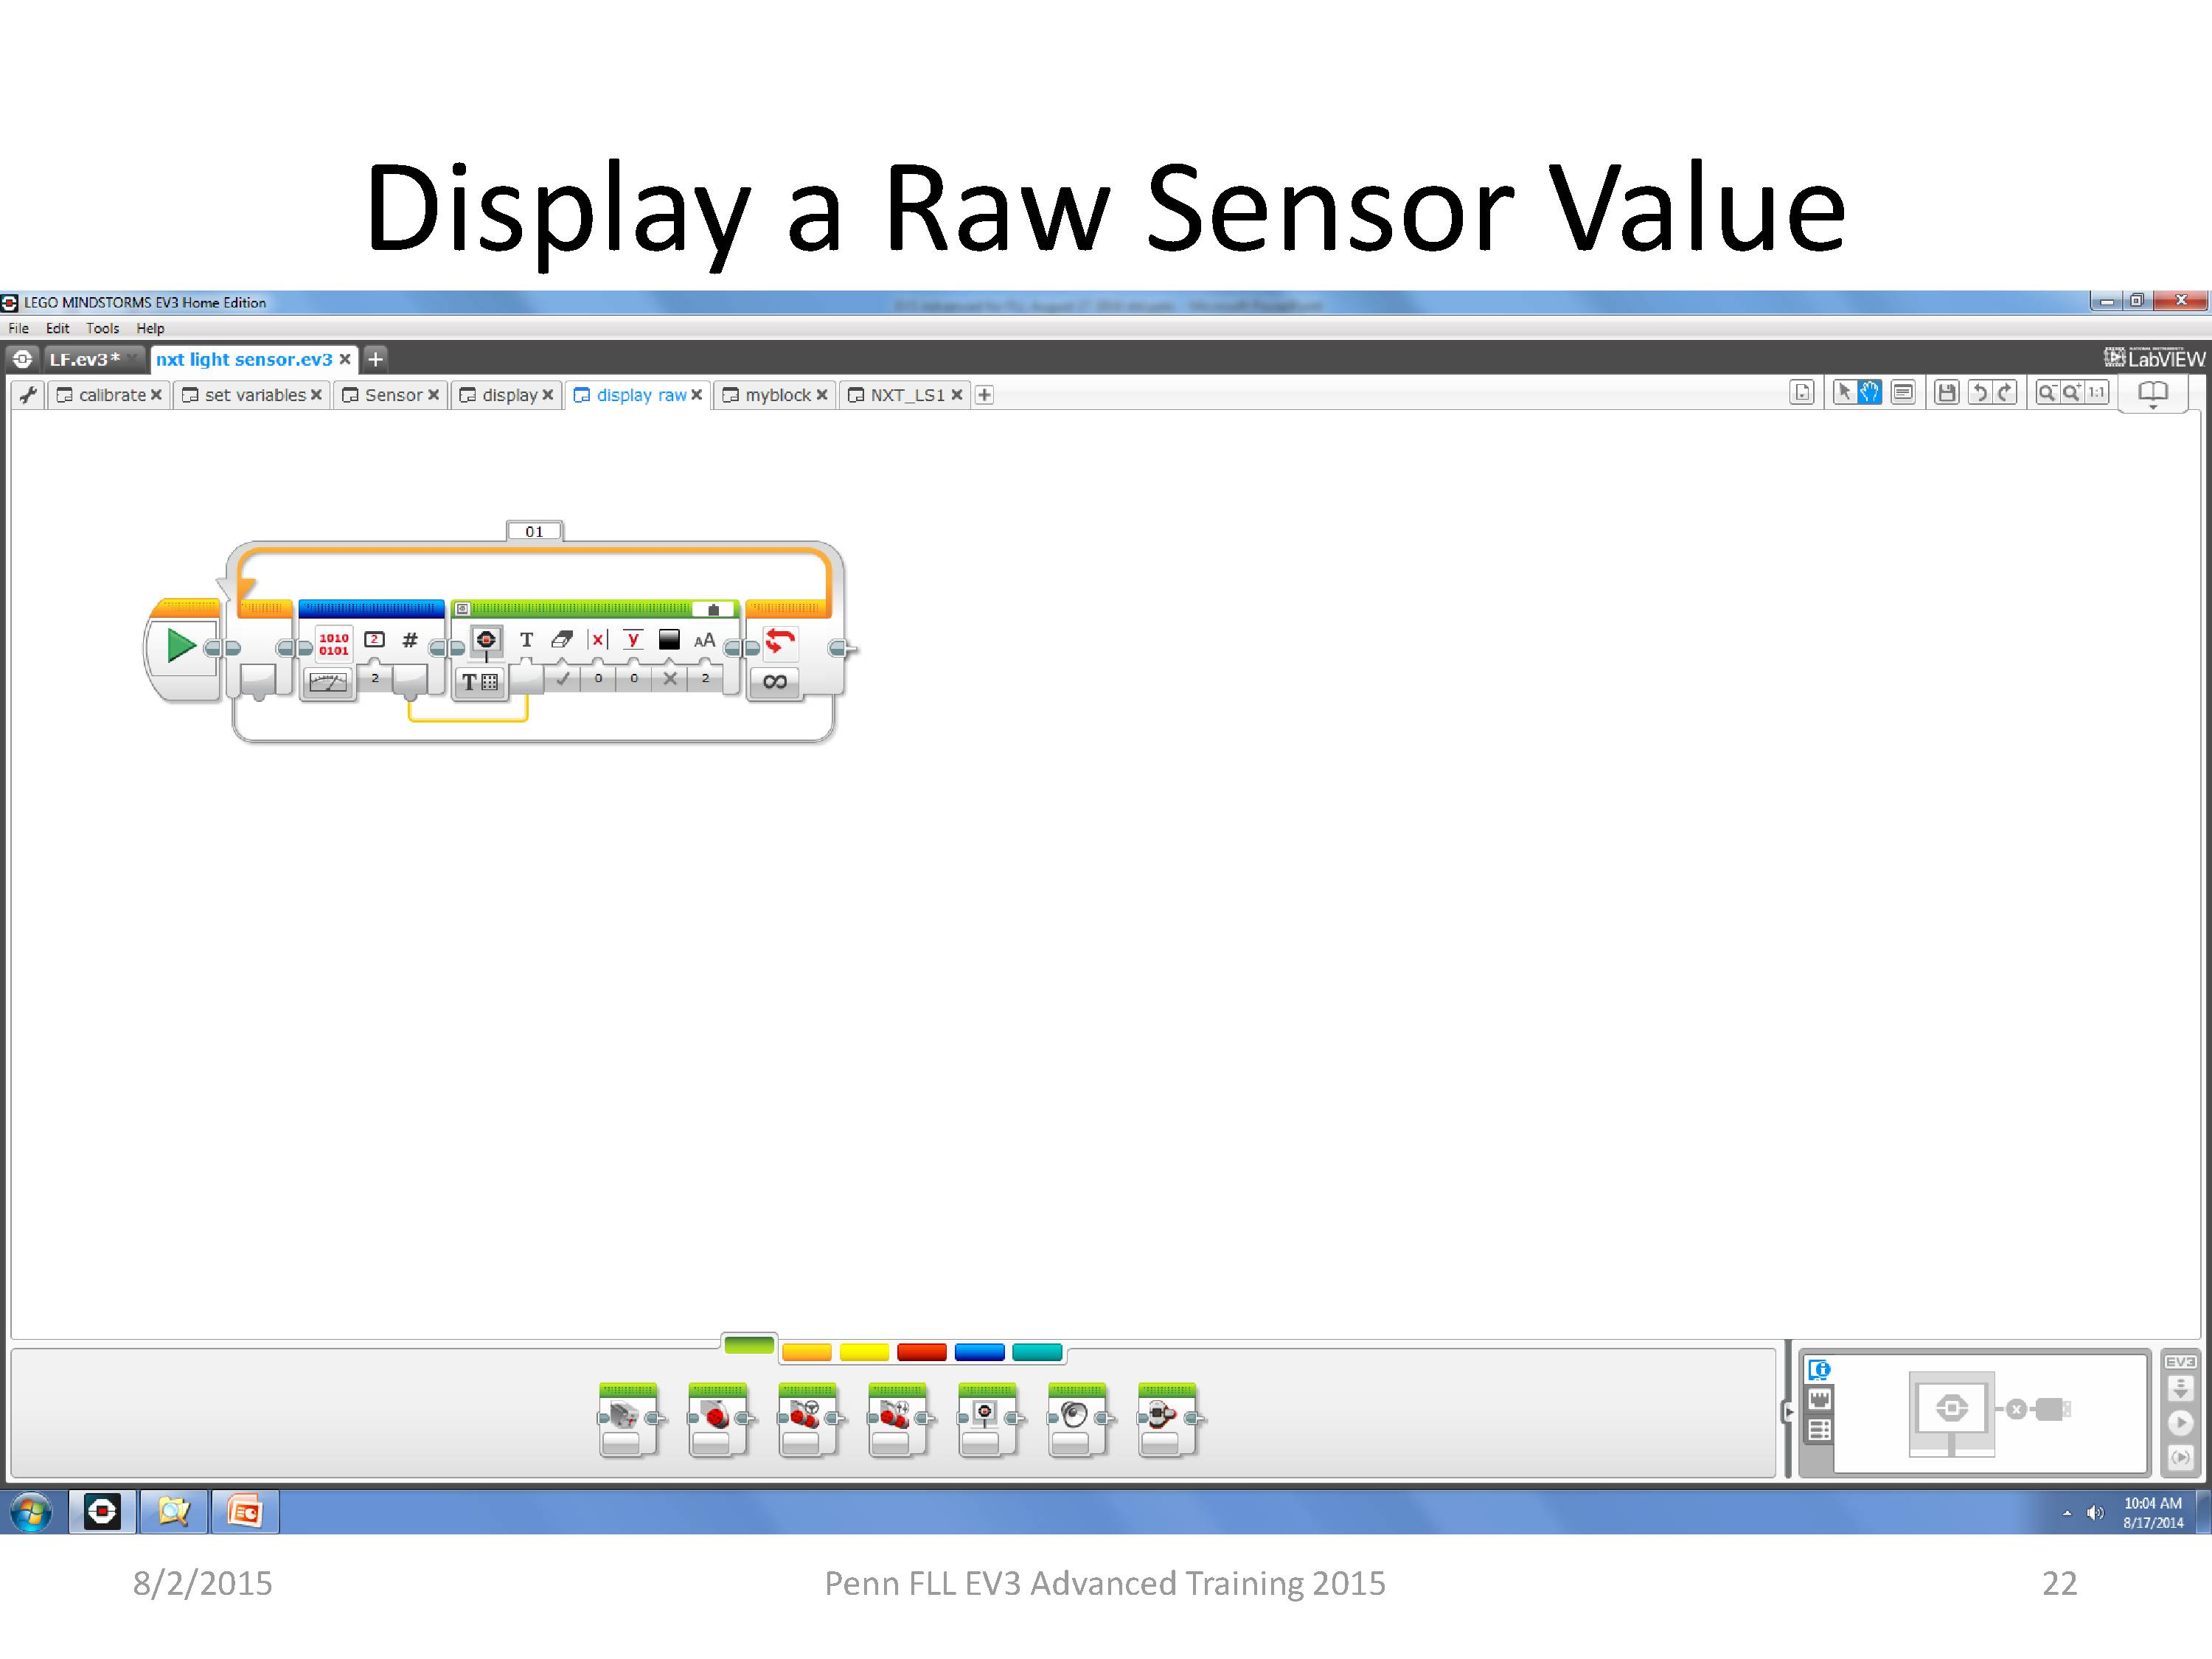
\includegraphics[scale=0.4]{ev3advanced2015/file-page22}
%\caption{lion!!}
\end{figure}
\end{frame}


\begin{frame}
%\frametitle{Pictures}
\begin{figure}
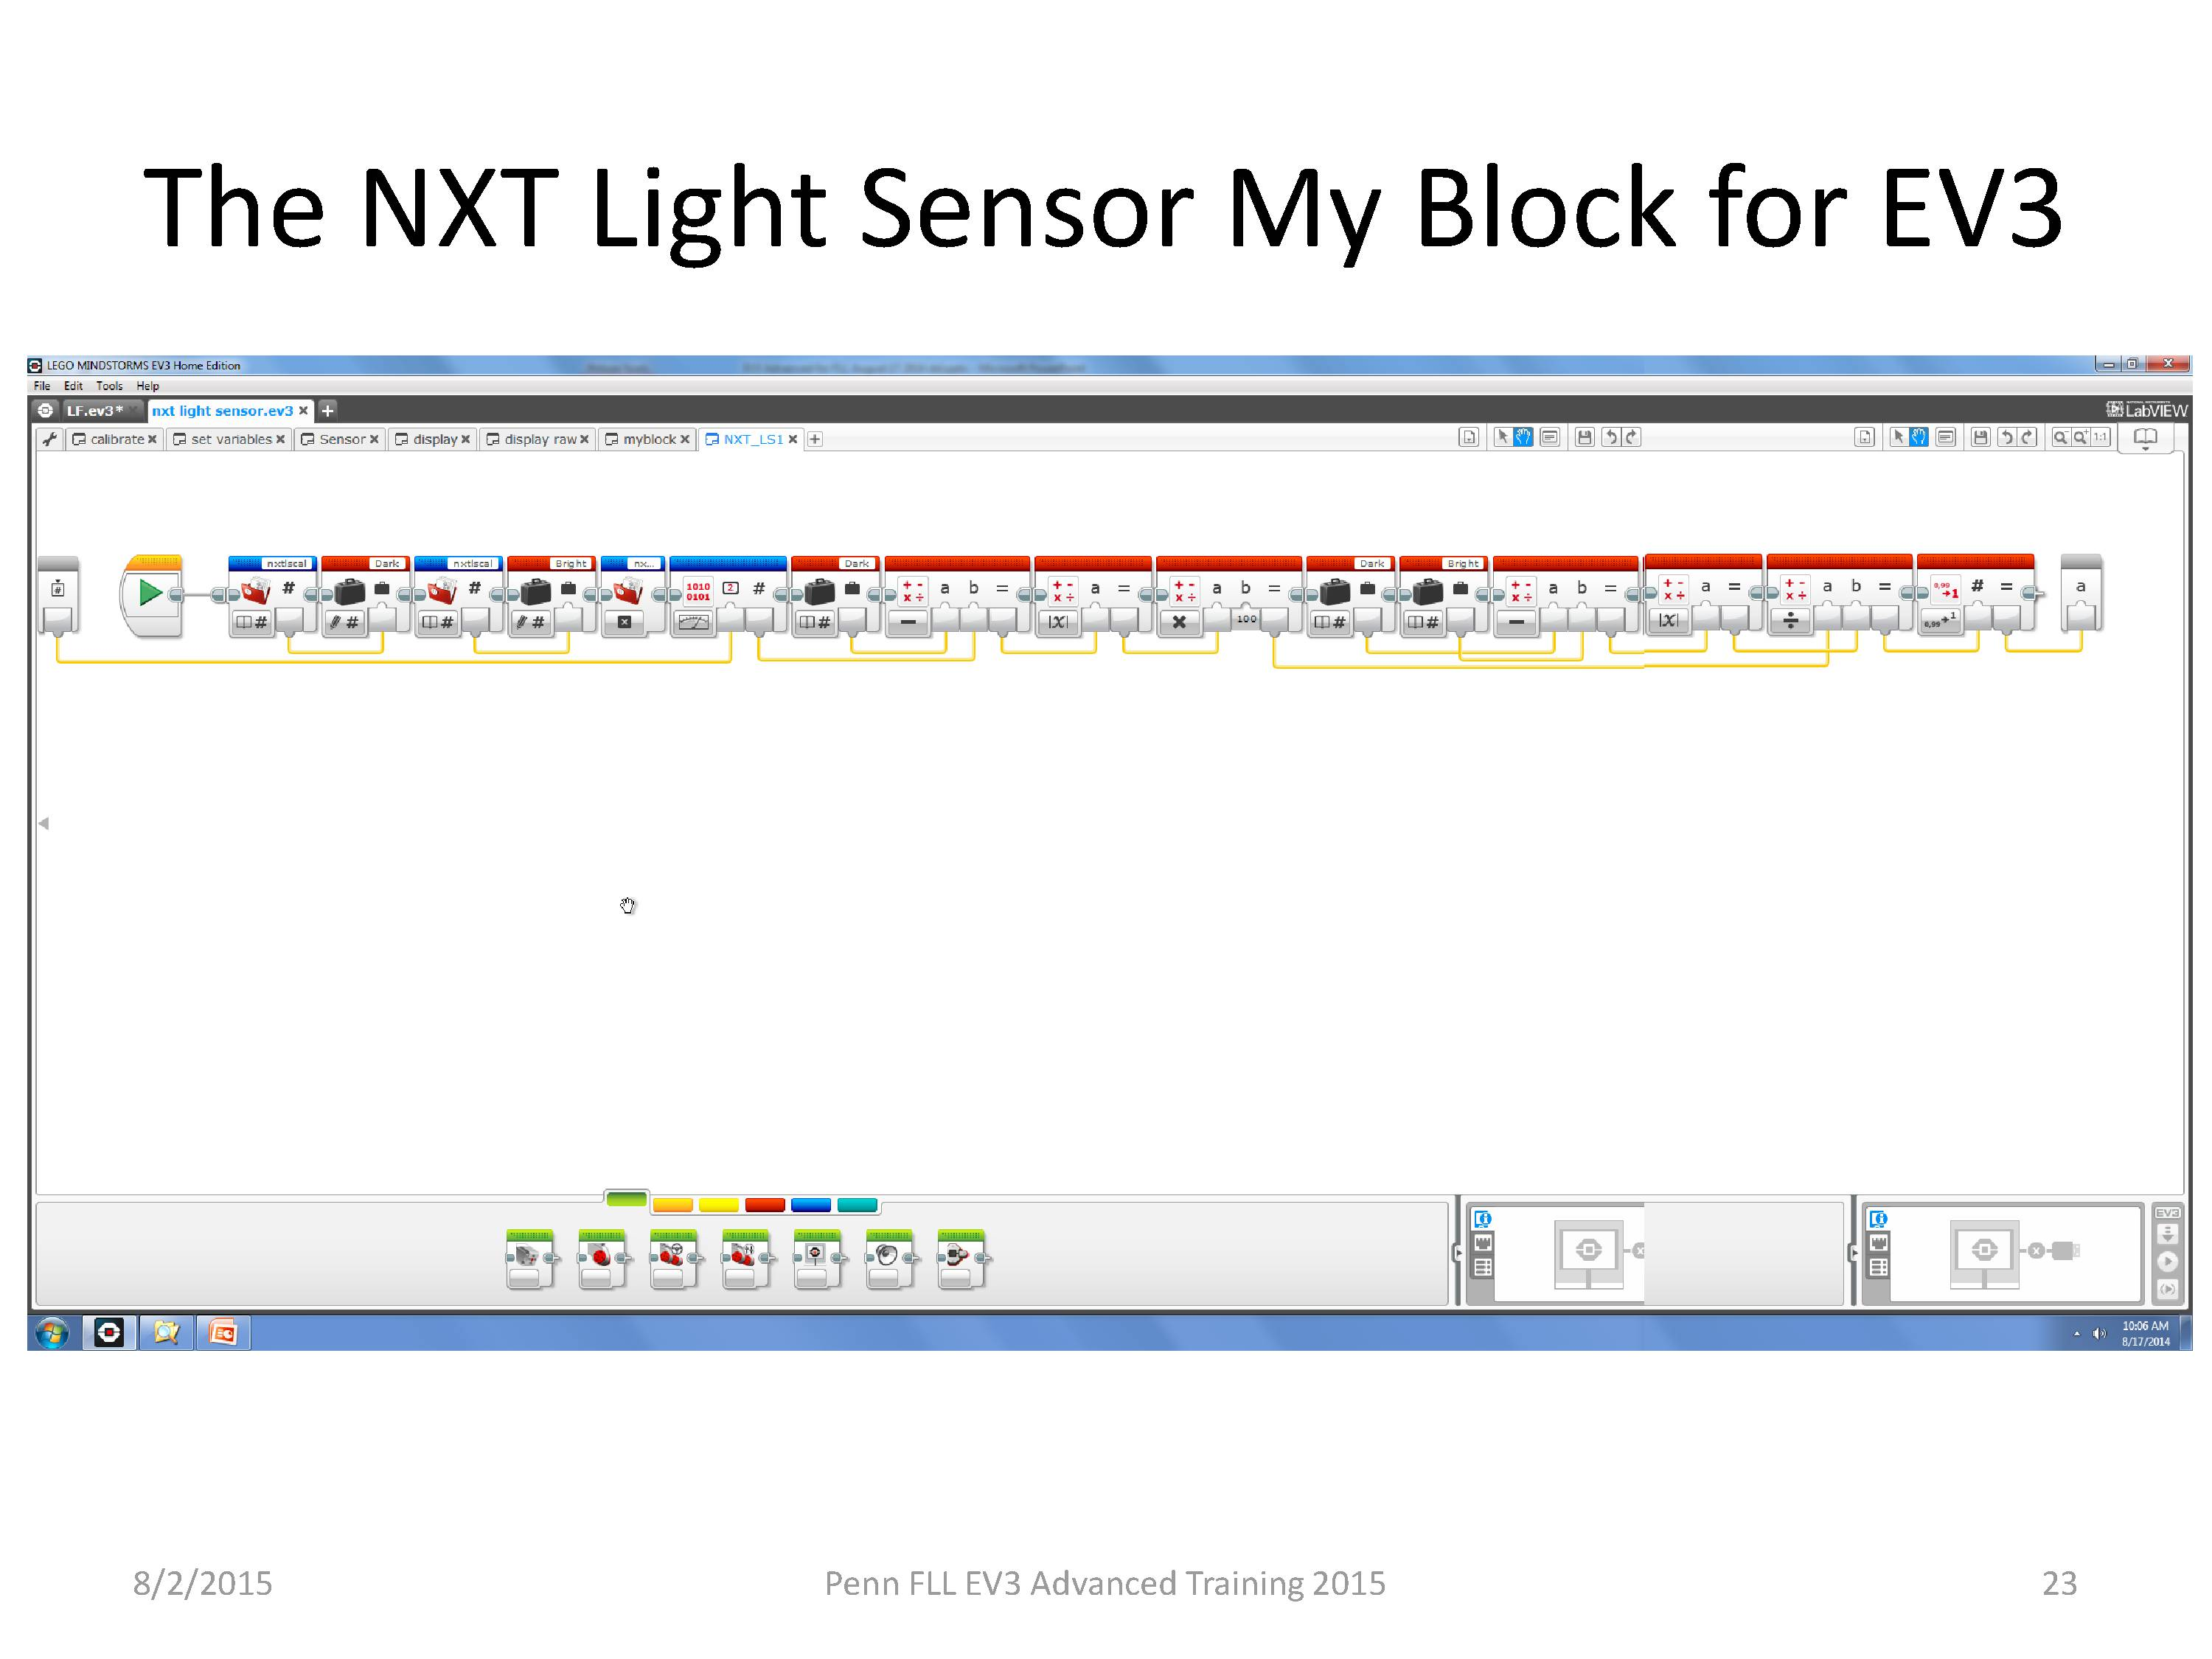
\includegraphics[scale=0.4]{ev3advanced2015/file-page23}
%\caption{lion!!}
\end{figure}
\end{frame}

\begin{frame}
%\frametitle{Pictures}
\begin{figure}
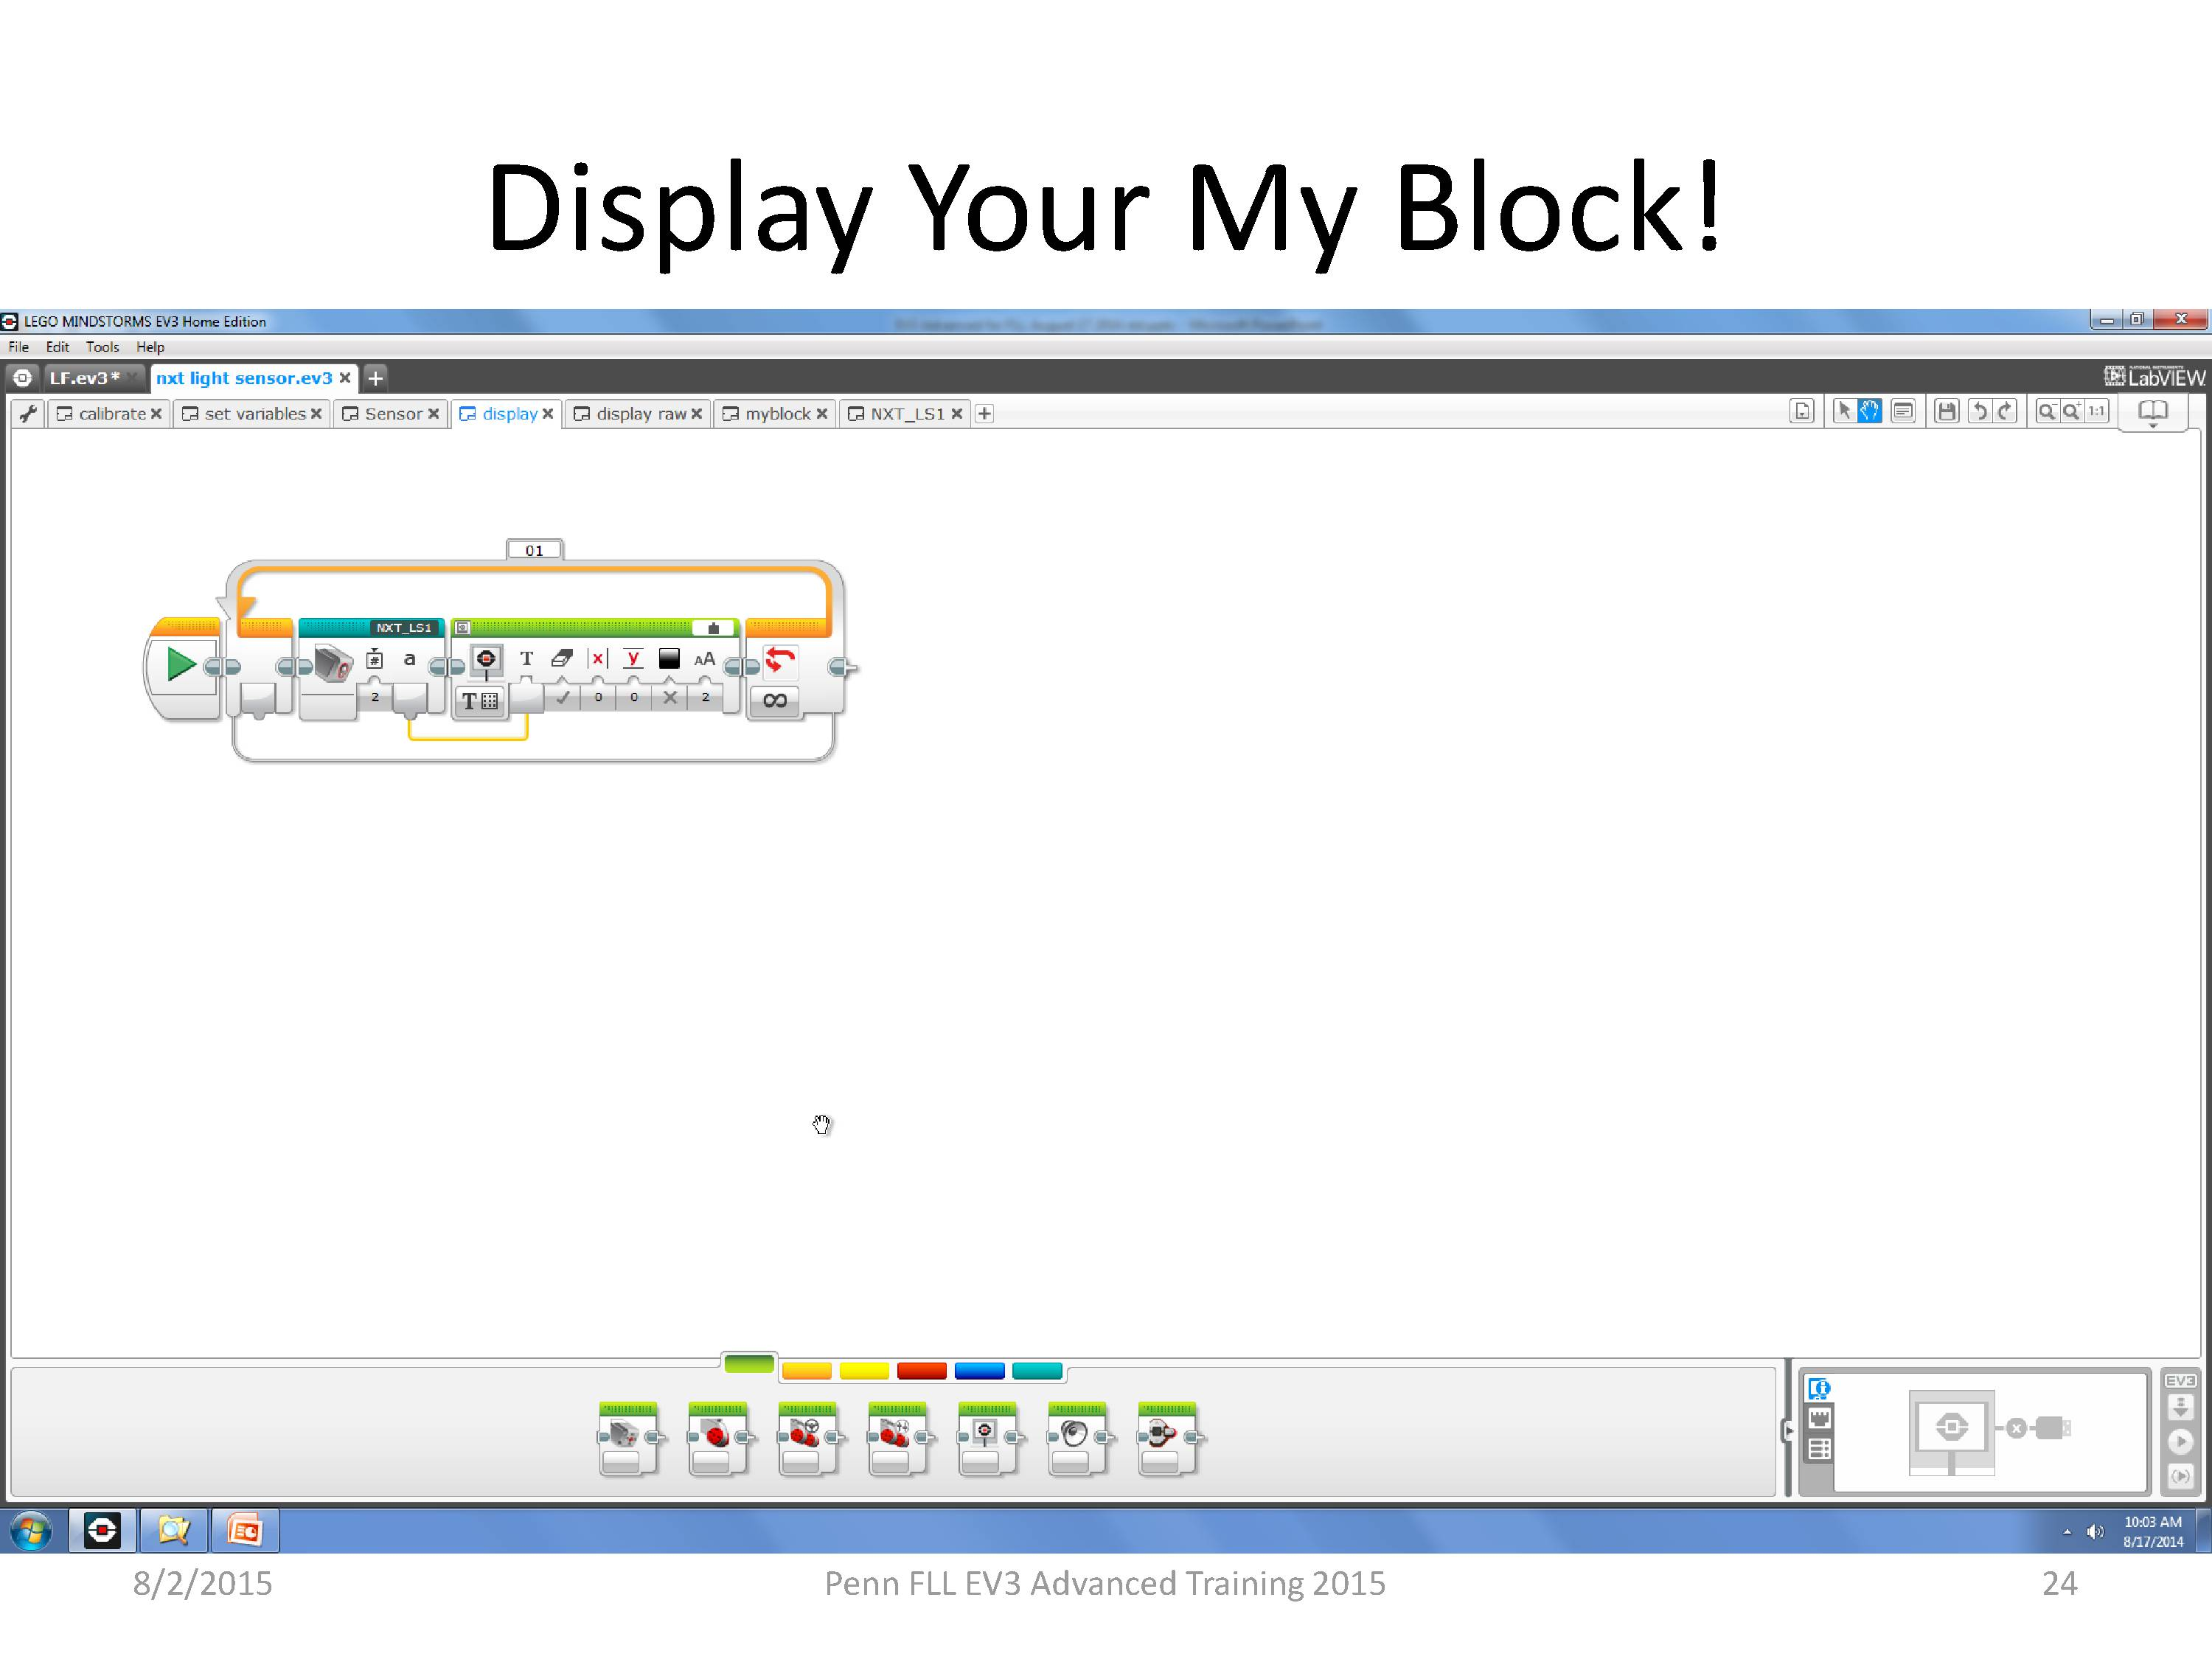
\includegraphics[scale=0.4]{ev3advanced2015/file-page24}
%\caption{lion!!}
\end{figure}
\end{frame}









\end{document}